%%%%%%%%%%%%%%%%%%%%%%% file template.tex %%%%%%%%%%%%%%%%%%%%%%%%%
%
% This is a general template file for the LaTeX package SVJour3
% for Springer journals.          Springer Heidelberg 2010/09/16
%
% Copy it to a new file with a new name and use it as the basis
% for your article. Delete % signs as needed.
%
% This template includes a few options for different layouts and
% content for various journals. Please consult a previous issue of
% your journal as needed.
%
%%%%%%%%%%%%%%%%%%%%%%%%%%%%%%%%%%%%%%%%%%%%%%%%%%%%%%%%%%%%%%%%%%%
%
% First comes an example EPS file -- just ignore it and
% proceed on the \documentclass line
% your LaTeX will extract the file if required
\begin{filecontents*}{example.eps}
	%!PS-Adobe-3.0 EPSF-3.0
	%%BoundingBox: 19 19 221 221
	%%CreationDate: Mon Sep 29 1997
	%%Creator: programmed by hand (JK)
	%%EndComments
	gsave
	newpath
	20 20 moveto
	20 220 lineto
	220 220 lineto
	220 20 lineto
	closepath
	2 setlinewidth
	gsave
	.4 setgray fill
	grestore
	stroke
	grestore
\end{filecontents*}
%
\RequirePackage{fix-cm}
\documentclass[twocolumn]{svjour3}          % twocolumn
%
\smartqed  % flush right qed marks, e.g. at end of proof
%
\usepackage{graphicx}

\usepackage{epstopdf}% To incorporate .eps illustrations using PDFLaTeX, etc.

\usepackage[noadjust]{cite}
\usepackage{graphicx}                
\usepackage{array,graphicx,float,caption}
\usepackage{subcaption}
\captionsetup{compatibility=false}
\usepackage{overpic}

\usepackage{booktabs}
\usepackage[normalem]{ulem}
% packages needed for Perla's commands
\usepackage{color}
\usepackage{soul}
\usepackage{svg}
\usepackage{array, amsmath}

\usepackage[numbers,sort&compress]{natbib}% Citation support using natbib.sty
\bibpunct[, ]{[}{]}{,}{n}{,}{,}% Citation support using natbib.sty
\renewcommand\bibfont{\fontsize{10}{12}\selectfont}% Bibliography support using natbib.sty
\makeatletter% @ becomes a letter
\def\NAT@def@citea{\def\@citea{\NAT@separator}}% Suppress spaces between citations using natbib.sty
\makeatother% @ becomes a symbol again



\newcommand{\degree}{$^{\circ}$ }%

% \usepackage{mathptmx}      % use Times fonts if available on your TeX system
%
% insert here the call for the packages your document requires
%\usepackage{latexsym}
% etc.
%
% please place your own definitions here and don't use \def but
% \newcommand{}{}
%
% Insert the name of "your journal" with
% \journalname{myjournal}
%
\begin{document}
	
%Commands defined by Perla
\newcommand{\DelP}[1]{\textcolor{red}{\st{#1}}}
\newcommand{\AddP}[1]{\textcolor{blue}{#1}}
\newcommand{\NoteP}[1]{\textcolor{green}{#1}}
\newcommand{\ULsubfloat}[2][\empty]% #1 = caption (optional), #2 = image
%\articletype{ARTICLE TEMPLATE}% Specify the article type or omit as appropriate
%\renewcommand{\footnote}{\number{footnote}}


\title{Structuring of Tactile Sensory Information for Category Formation in Robotics Palpation.
	\thanks{This work was funded by the UK Agriculture and Horticulture Development
		Board and by The United Kingdom Engineering and Physical Sciences
		Research Council (EPSRC) MOTION grant [EP/N03211X/2].}
}

%\titlerunning{Short form of title}        % if too long for running head

\author{Luca Scimeca $^{1}$          		\and
	Perla Maiolino $^{1}$ 	 			\and
	Ed Bray $^{1}$			 			\and
	Fumiya Iida $^{1}$ 	 			\and %etc.
}

%\authorrunning{Short form of author list} % if too long for running head

\institute{
	Luca Scimeca	\at
	\email{ls769@cam.ac.uk} \and Perla Maiolino \at	\email{pm640@cam.ac.uk} \and
	$^{1}$ Bioinspired Robotic Lab, Engineering Department, $\text{University}$ of Cambridge, Cambridge UK
}

\date{Received: date / Accepted: date}

\maketitle
\begin{abstract}
	\color{red}{This paper proposes a framework to investigate the influence of physical interactions to sensory information, during robotic palpation. We embed a capacitive tactile sensor on a robotic arm to probe a soft phantom and detect and classify hard inclusions within it. A combination of PCA and K-Means clustering is used to: 
	first, reduce the dimensionality of the spatiotemporal data obtained through the probing of each area in the phantom; 
	second categorize the re-encoded data into a given number of categories. Results show that appropriate probing 
	interactions can be useful in compensating for the quality of the data, or lack thereof. Finally, we test the proposed framework on a palpation scenario where a Support Vector Machine classifier is trained to discriminate amongst different types of hard inclusions. We show the proposed framework is capable of predicting the best-performing motion strategy, as well as the relative classification performance of the SVM classifier, solely based on unsupervised cluster analysis methods.}
\end{abstract}

\keywords{Robotic palpation, Tactile sensing, physical sensing, Sensory-Motor coordination}  

\section{Introduction}
In the last decades, substantial efforts have been made in enhancing the sensing capabilities 
of robots by providing them with a sense of touch \cite{dahiya_tactile_2010, drimus2014design}. Haptic sensing differs 
from other modalities, such as vision, in virtue of its tight coupling with, and need of, physical interactions. 
Haptic sensing requires direct physical contacts with sensing targets, inducing spatio-temporal force patterns 
on the contact surface, which may or may not be the consequence of motor behaviors of the robots. 
Furthermore, force patterns are significantly related to the shape and mechanical properties of sensing 
surfaces (e.g. stiffness) and the target objects \cite{scimecasoft, fumiya_2016}. 

In medical palpation diagnosis, for example, given the nature of soft tissues in the human body, 
haptic perception plays a fundamental role \cite{puangmali2008state}. 
Here, practitioners necessitate the use of different palpation strategies according to the task, whether 
this is an organ to examine, finding cancerous inclusions or 
investigating their characteristics. In this context, contacts and physical interactions are the basis of rich sensory 
stimuli, with which practitioners can judge the conditions of target areas \cite{palpation1,palpation2,palpation3}.
Indeed, previous research has focused on the use of haptics for RMIS and medical training \cite{mclaughlin2002introduction}. 
These systems, currently based on vision, can be augmented with tactile information, improving the ability of surgeons 
to detect the mechanical properties of touched organs, and help in the localization of tumors and lumps \cite{Liza2014}.

The strong dependence between the somatosensory system and motor actions in human palpation has been investigated 
in relation to the development of robotic palpation systems for detection of hard inclusions \cite{Liza2014behavioral,sornkarn2016efficacy, yen2003palpation, konstantinova2017palpation, herzig2018variable}. 
\color{red}{ In the context of hard inclusion detection, the structure of sensory stimuli generated physical palpation, helps to understand similarities or differences amongst the palpated objects. Through pertinent physical interactions, sensory stimuli of similar objects will maintain strong invariant similarities in the sensing space, whilst increasing their difference with dissimilar objects. In this context, the invariances allow for the dissociation of stimuli originated from different objects and the association, instead, of stimuli derived from similar objects. This fundamental process, corresponding to the separation and association of sensor stimuli into groups, will be referred to as categorization.
%	The number of groups, to divide the sensor space into, sets the level of abstraction intended for the understanding of the sensor information. 


%Through pertinent physical interactions, sensor information relative to 
%similar objects will maintain strong invariant similarities in the sensor space, whilst dissimilar objects will increase
%their .

%of robotic palpation systems for detection of hard inclusions \cite{Liza2014,Liza2014behavioral,sornkarn2016efficacy}  
%and it is considered of primary importance in the categorization behavior \cite{pfeifer1997}.
%This specific application scenario exemplifies the importance of sensory-motor coordination for discriminating between 
%sensory stimuli because what is experienced by the practitioner strongly depends by the cross coupling between the 
%somatosensory system and the motor action. This aspect has been strongly investigated in relation to the development 
%of robotic palpation systems for detection of hard inclusions \cite{Liza2014,Liza2014behavioral,sornkarn2016efficacy}  
%and it is considered of primary importance in the categorization behavior \cite{pfeifer1997}. In particular the 
%sensory-motor coordination theory \cite{lungarella2005methods,pfeifer2007information} includes three types of 
%processes: i) physical, or active, sensing, ii) dimensionality reduction processes, and iii) processes capable of 
%differentiating between different stimuli.
%
%% SMC
%First, active interaction can directly select or influence the perceived sensory patterns. The consequences of motion 
%to the perceived stimuli have been the focus of much work in the past years, where research has shown how said 
%influence can actively improve the ability to retrieve information from the world and induce structure for simplified 
%information processing (information self-structuring) \cite{pfeifer2007information}. However, accounting for motor 
%interaction induces the rich spatio-temporal information retrieved to be often redundant and highly dimensional.
%
%% dimensionality reduction & Cognitive map
%
%Second, dimensionality reduction processes are necessary to pass from a set of highly dimensional sensor information 
%to a subset of invariant properties of the sensory signal. These invariances, should both fundamentally describe the 
%stimulus perceived, and differentiate it from other, possibly similar, stimuli. 
%
%In biological organism the mapping process between stimulus perceived and its representation is referred to as cognitive 
%mapping, from which a cognitive map is produced \cite{cognitive,wong2007}. In this paper, we refer to a cognitive map as 
%a mathematical, minimalistic, representation method for sensory stimuli that identify the mapping between high dimensional 
%spatio-temporal stimuli to lower dimensional encoding of the same. 
%
%% Categorization and Category formation, MAYBE say LESS ?

%Third, 
%category formation is the separation in the sensor space of the sensor stimuli.

\begin{figure*}[]
	\centering
	\begin{subfigure}[b]{.448\textwidth}
		\centering
		\includegraphics[width=\textwidth]{./figs/set_up.eps}
		\caption{Robot set-up}
		\label{exp:robot}
	\end{subfigure}
	\hspace{0.01\textwidth}
	\begin{subfigure}[b]{0.53\textwidth}
		\begin{subfigure}[b]{\textwidth}
			\centering
			\begin{subfigure}[b]{.45\textwidth}
				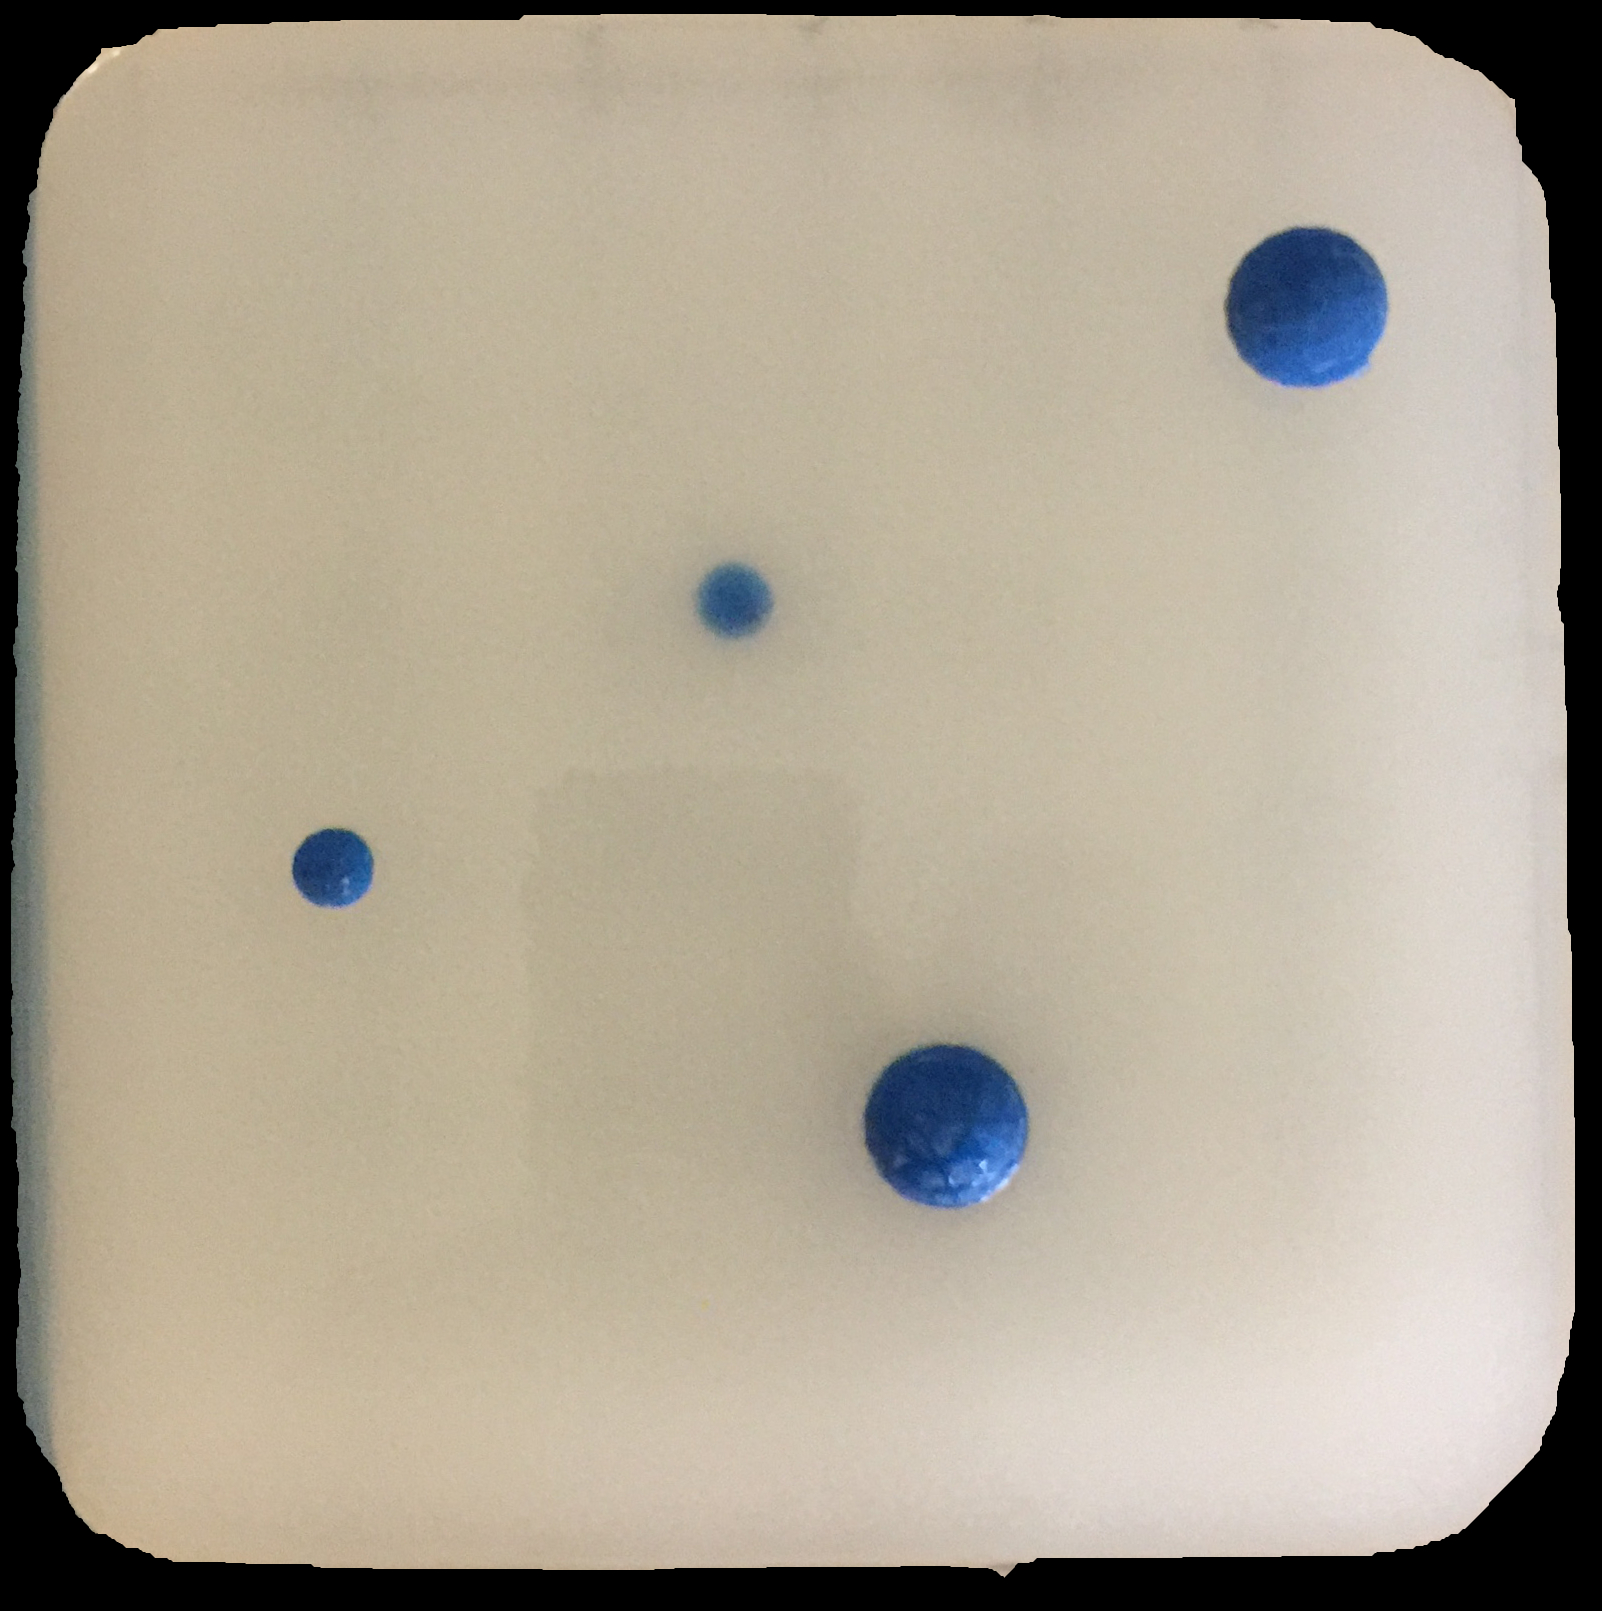
\includegraphics[width=\textwidth]{./figs/phantom.jpg}
				\caption{$Ph\text{-}1$}
				\label{ph1}
			\end{subfigure}
			\hspace{0.01\textwidth}
			\begin{subfigure}[b]{.46\textwidth}
				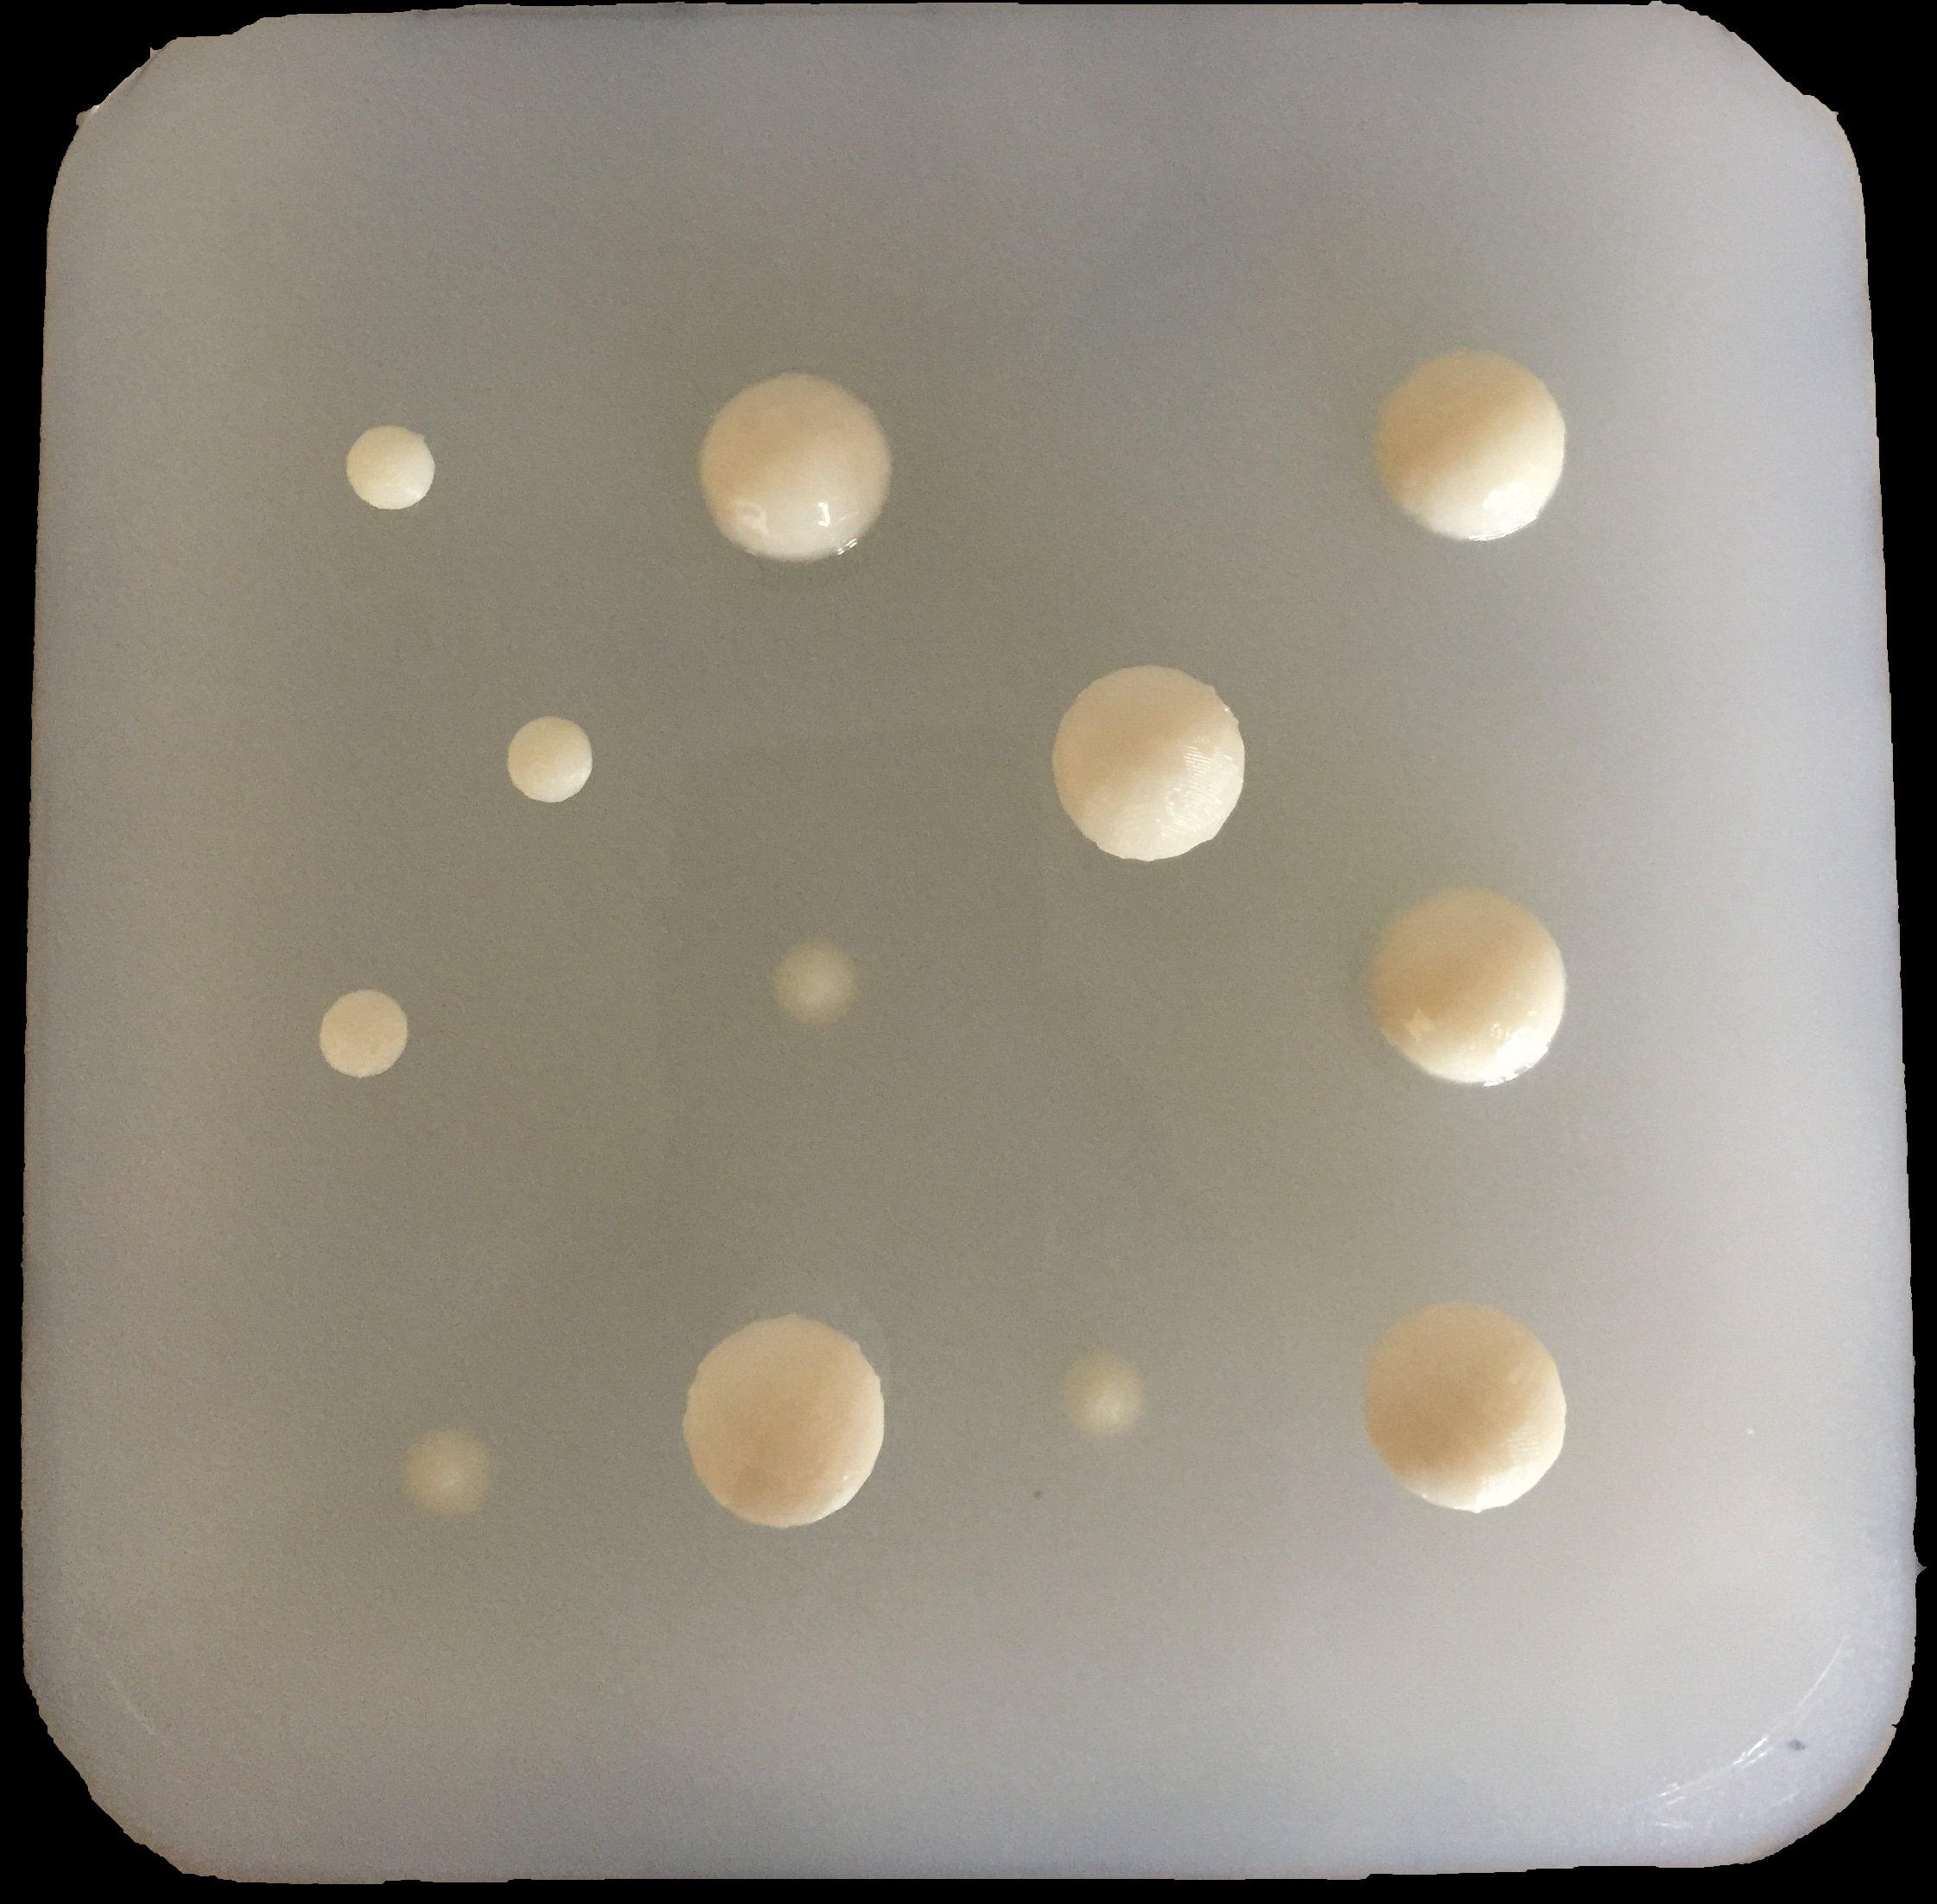
\includegraphics[width=\textwidth]{./figs/ph2.jpg}
				\caption{$Ph\text{-}2$}
				\label{ph2}
			\end{subfigure}
		\end{subfigure}
		
		\begin{subfigure}[b]{\textwidth}
			\centering
			\begin{subfigure}[b]{0.51\textwidth}
				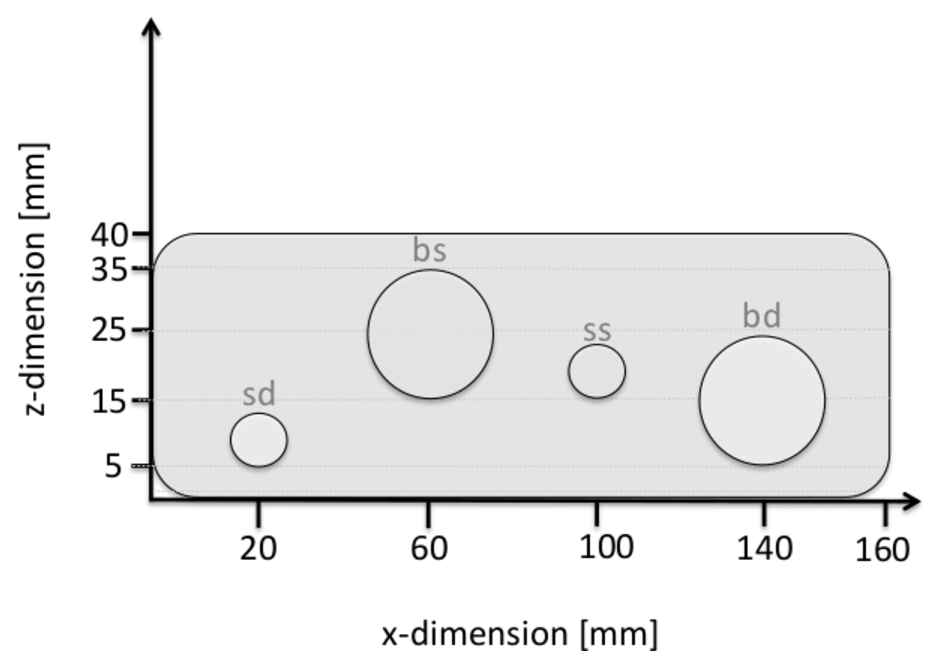
\includegraphics[width=\textwidth]{./figs/phside.eps}
				\caption{Inclusion types}
				\label{phantomgrid:description}
				%			\vspace{12pt}
			\end{subfigure}
			\begin{subfigure}[b]{0.46\textwidth}
				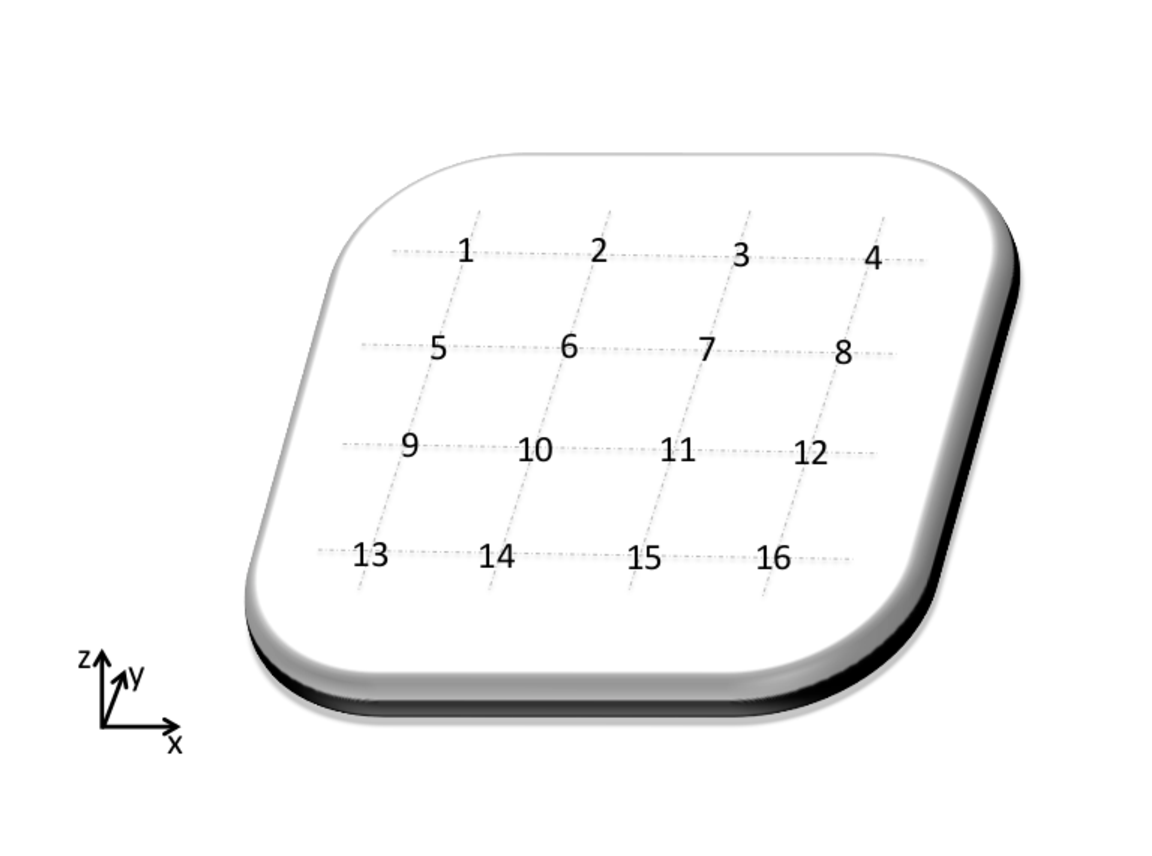
\includegraphics[width=\textwidth]{./figs/phlocations.eps}
				\caption{Phantom grids}
				\label{phantomgrid:3d}
			\end{subfigure} 
		\end{subfigure}
	\end{subfigure}
	\caption{}
	\label{robot-set-up}
	
\end{figure*}
% Problem statement
The importance of categorization has previously been emphasized in \cite{hoffmann2012implications}, and the use of active 
interactions to solve the categorization problem has been explored in previous research 
\cite{pfeifer1997, nolfi2002active, tuci2009dynamics}.
Considering the problem of categorization in the scenario of robotic palpation systems, much is still unclear. 
This paper addresses two related problems. First, we wish to understand how motor actions can aid in the separation and categorization of tactile sensor information. Research has previously shown that motor actions can introduce structure in sensory information \cite{lungarella2005methods, sporns2006evolving, pfeifer2007information}, but it is yet to be understood 
which principles guide the emergence of such structure. Second, as later shown in this paper, knowing the task to solve may not be enough to understand which physical interaction strategy is appropriate to use, or predict its effects to the tactile information. Here, instead, it is first necessary to understand the properties of the objects in interaction with the agent and the level of abstraction intended for the categorization.

% contribution
In order to address the above problems this paper investigates the processing of sensor signals based on dimensionality 
reduction and clustering. We propose a framework to explore the way active physical interactions with a soft body affect the structure of haptic spatio-temporal information. Through the proposed framework it is thus possible to choose in which way it is most appropriate to interact with objects, to improve their categorization and thus solve a classification task. The task, in this scenario, is the detection and classification of hard inclusions within a robotic palpation system.

% structure of this paper
The paper is organized as follows: In Section \ref{sec_methods} we describe the methods used, starting from the experimental 
set-up in Section \ref{sec_experimental_setups}, to the acquisition of tactile data though various probing strategies in sections \ref{sec_skin} and \ref{sec_motor_interactions}. In Section \ref{sec_th_framework} we describe the proposed framework. In Section \ref{sec_results} we report the results of the experiments followed by a case study in Section \ref{sec_test_case} and the conclusion in section  \ref{sec_conclusion}. } \color{black}



%############# METHODS###########
\section{Methods} \label{sec_methods}
\color{red}We arrange an experimental scenario where a robotic arm, equipped with an end-effector and a tactile sensor, probes the soft tissue of a soft phantom organ, to detect hard inclusions within it. The properties of the phantom organ designed to test the ability of the robotic agent to be detect hard inclusions by their depth and size, as shown to be important in previous systems~\cite{herzig2018variable}.
%By changing the probing strategy of the robot during the interactions with 
%the soft phantom, the sensory response of the sensorised probe changes, modifying the retrieved data
%and consequently the discretization of the tactile information into categories (Fig. \ref{self_org_processing}). 
\color{black}

\subsection{Soft Phantom and Robot Set-Up} \label{sec_experimental_setups}
We built two $160\text{x}160\text{x}40mm$ soft phantom organs using Ecoflex 00-10\footnote[2]
{https://www.smooth-on.com/products/ecoflex-00-10/} from Smooth-on. The phantom organs are divided in 16 
locations disposed in a coarse grained grid system as shown in Fig. \ref{phantomgrid:3d}. Each location in the 
phantoms may or may not contain hard inclusions. An inclusion consists of a 3D-printed hard, spherical bead, 
embedded in the phantoms at a depth of either $5mm$ or $15mm$, and having a diameter of 
$7mm$ or $20mm$ (Fig. \ref{phantomgrid:description}). Hereafter we may refer to a $7mm$ inclusion 
placed at a depth of $5mm$ as \textit{SS} (Small-Shallow), a $20mm$ inclusion placed at $5mm$ as \textit{BS} 
(Big-Shallow), a $7mm$ inclusion placed at $15mm$ as \textit{SD} (Small-Deep), a $20mm$ inclusion placed at 
$15mm$ as \textit{BD} (Big-Deep) and an area containing no hard inclusions as \textit{NA}.

The experiments were performed on two phantoms: $Ph\text{-}1$, containing $12\text{x}$\textit{NA}, $1\text{x}$\textit{SD}, $1\text{x}$\textit{SS}, $1\text{x}$\textit{BS}, $1\text{x}$\textit{BD} (Fig. \ref{ph1}); and $Ph\text{-}2$, containing $4\text{x}$\textit{NA}, $3\text{x}$\textit{SD}, $3\text{x}$\textit{SS}, $3\text{x}$\textit{BS}, $3\text{x}$\textit{BD} (Fig. \ref{ph2}).

We 3D-printed a custom-made end-effector and integrated a capacitive tactile sensor onto its 
surface to retrieve $tactile\ images$ during the probing experiments (Fig. \ref{CySkin:probe}). 
The printed end-effector, coupled with the tactile sensor, was mounted onto an ST-Robotics R12/5 robotic 
arm\footnote[3]{http://www.robotshop.com/uk/st-robotics-r12-5-axis-articulated-robot-arm.html}   
(Fig. \ref{exp:robot}). 

\subsection{Tactile Sensor Technology and Data Acquisition} \label{sec_skin}
High spatial resolution is a crucial component of the sensor technology necessary for the 
analysis in this paper. The tactile sensor used is described in \cite{schmitz_methods_2011}. 
The adopted sensing mode is based on the capacitive transduction principle. 
A capacitive transducer (i.e., a tactile element, or $taxel$) is organized in a 
layered structure: the lower layer consists of the positive electrode, which is mounted 
on a Flexible Printed Circuit Board (FPCB); a small air chamber act as dielectric and the 
upper layer is a ground plane made with conductive lycra. The tactile sensor is made up 
of a number of taxels geometrically organized in triangular modules. 

In the current prototype, each module hosts $7$ taxels (Fig. \ref{CySkin:probe}), as well as 
the Capacitance to Digital Converter (CDC) chip (namely, the AD7147 from Analog Devices) for 
converting capacitance values to digital. The CDC chip can measure variations in capacitance 
values with 16 bits of resolution. All the modules are interconnected and communicate through 
an SPI bus to a read-out board which performs a preliminary processing of the tactile sensor 
data and send them to the PC through CAN bus (Fig. \ref{CySkin:schema}) %within the $4 \div 30pF$ range 
with a sensitivity of $0.32fF$. 

In this context, the normal forces exerted on the sensor produce variations in capacitance 
values reflecting the varied pressure over the taxel positions. A sensor reading, or tactile 
image, from the tactile sensor described is produced at $20Hz$, and corresponds to 
a 7-dimensional array, where each element contains the capacitance variation value of 
the corresponding taxel.

%is $\Delta C_i$, and $i$ is its corresponding taxel in the sensor.
%When performing the experiments, the  tactile images are not used singularly. For every 
%probing strategy designed, we take series of sensor readings over equally spaced intervals, 
%and concatenate them sequentially into a single array (time series). In this paper we refer 
%to a tactile image sequence as the concatenated sensor readings after applying a specific 
%probing strategy.

\subsection{Probing Strategies} \label{sec_motor_interactions}

We control the r12/5 robotic arm open-loop in Cartesian coordinates. A teach-pendant was used to manually teach the 
robot the x-y location of the areas to probe. We use the stored end-effector positions in the subsequent 
control algorithm, where the robot automatically probes each location using the preferred probing strategy. 
We differentiate between two qualitatively different types of probing strategies, summarized in 
Fig. \ref{probing}: vertical and rotatory. 

First, the vertical probing strategy is performed with the probe aligned vertically and plunged 
directly down into the phantom at 0.5 mm increments. After each increment, the robot briefly pauses to allow a 
tactile image to be recorded before continuing with the next movement. This continues until the probe is at a 
depth $d$ below the surface of the silicon, whereupon it stops recording and returns to a neutral position 10 mm 
above the surface in a single movement.

Second, the rotary motion is performed with the robot $d$ mm below the surface of the silicone, rotating about 
a nexus point $r$ mm away in the vertical direction. To reach the initial position of this motion strategy, 
the robot moves vertically downward from its rest position, until it reaches the position set by $d$. Hence, a 
nexus point $r$ distant from the end effector is assumed, and the robot rotates about it in the $+\theta$ 
direction until it is at an angle of 30\degree from its initial, vertical, position. Here, the palpation action can 
begin. The probe rotates in the $-\theta$ direction at 1\degree increments, recording a tactile image after each step. 
Once the probe has rotated of 60\degree it stops recording, and returns to its rest position 10 mm above the 
surface of the silicone. 

In general, a probing strategy can be uniquely identified by a depth $d$ and a radius $r$, thus:
\begin{equation}
\Theta = \begin{Bmatrix}d\\ r\end{Bmatrix},
\end{equation} 
where if $r=0$, the probing motion will be vertical, while if $r>0$ the probing takes place via the 
rotatory strategy (Fig. \ref{probing}).




\begin{figure}[] 
	\centering
	%	\hspace{0.0005\columnwidth}
	\begin{subfigure}[b]{.685\columnwidth}
		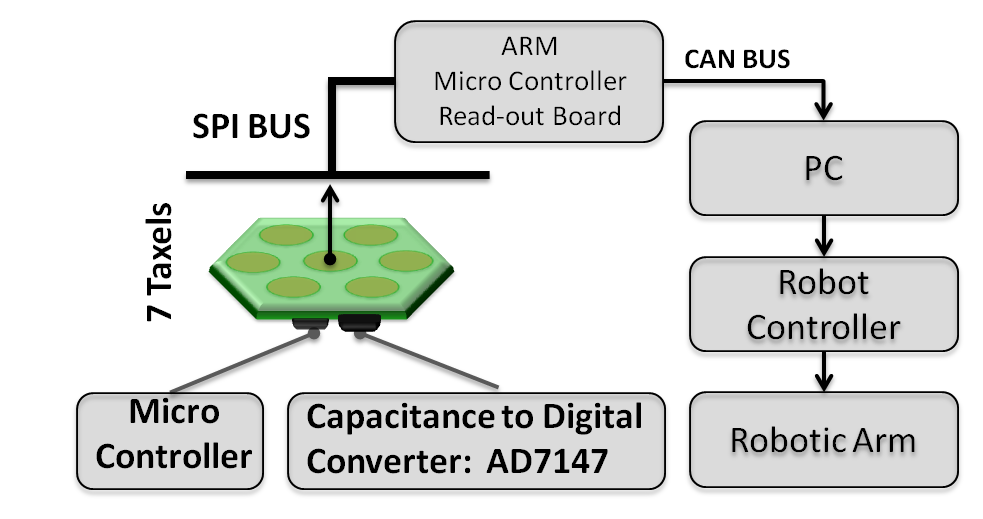
\includegraphics[width=\columnwidth]{./figs/Presentationarchitecture.eps}
		\caption{}
		\label{CySkin:schema}
	\end{subfigure} 
	\hspace{0.02\columnwidth}
	\begin{subfigure}[b]{0.27\columnwidth}
		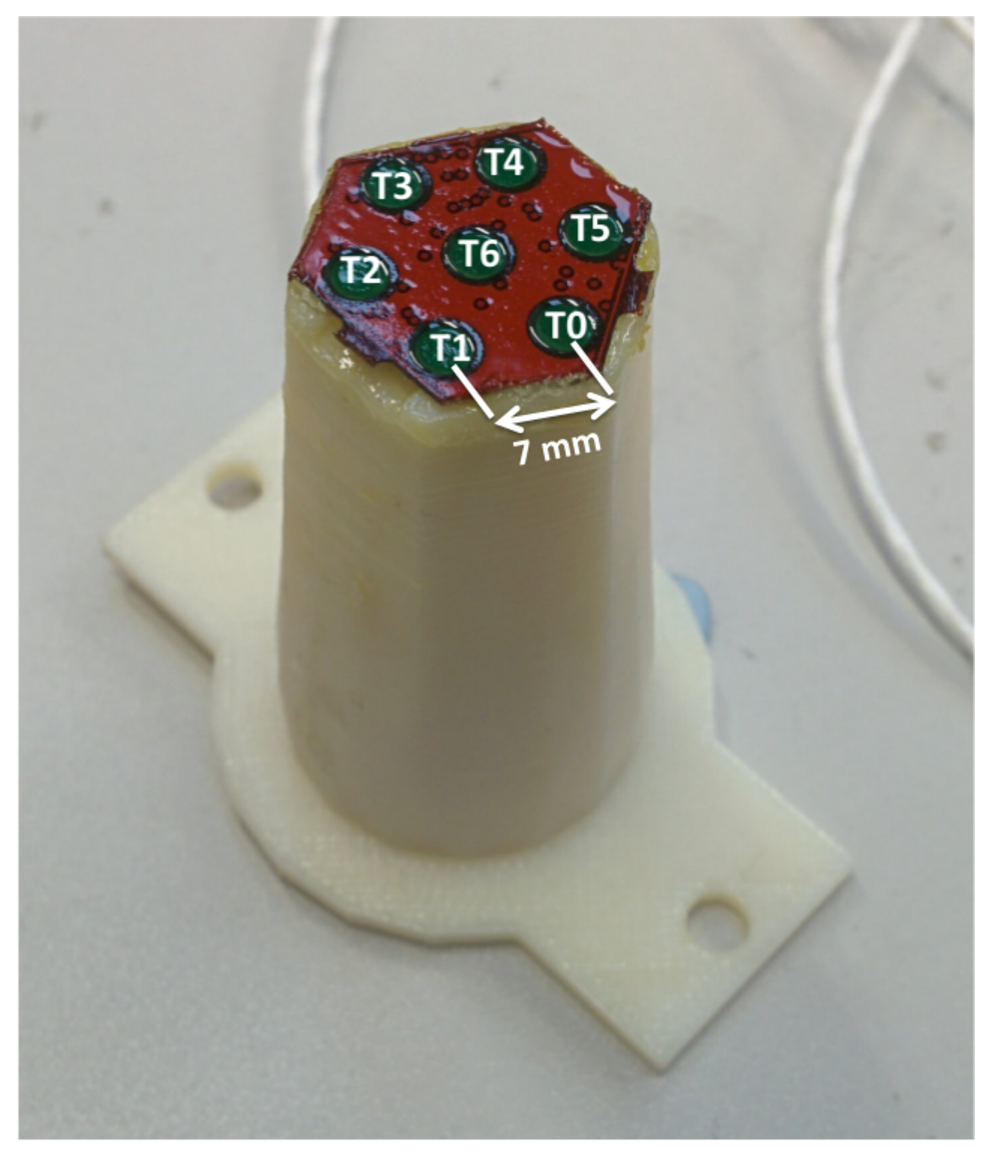
\includegraphics[width=\columnwidth]{./figs/probefreccia.eps}
		\caption{}
		\label{CySkin:probe}
	\end{subfigure}
	\caption{(a) The CySkin technology architecture. The hexagonal patch is connected to a 
		Intelligent Hub Board (IHB) that collect the tactile sensor data and send them to the 
		PC through a CAN bus. (b) The sensorised probe coupled with the CySkin patch used for 
		the experiments. }
	\label{CySkin}
\end{figure}
\begin{figure}[]
	\centering
	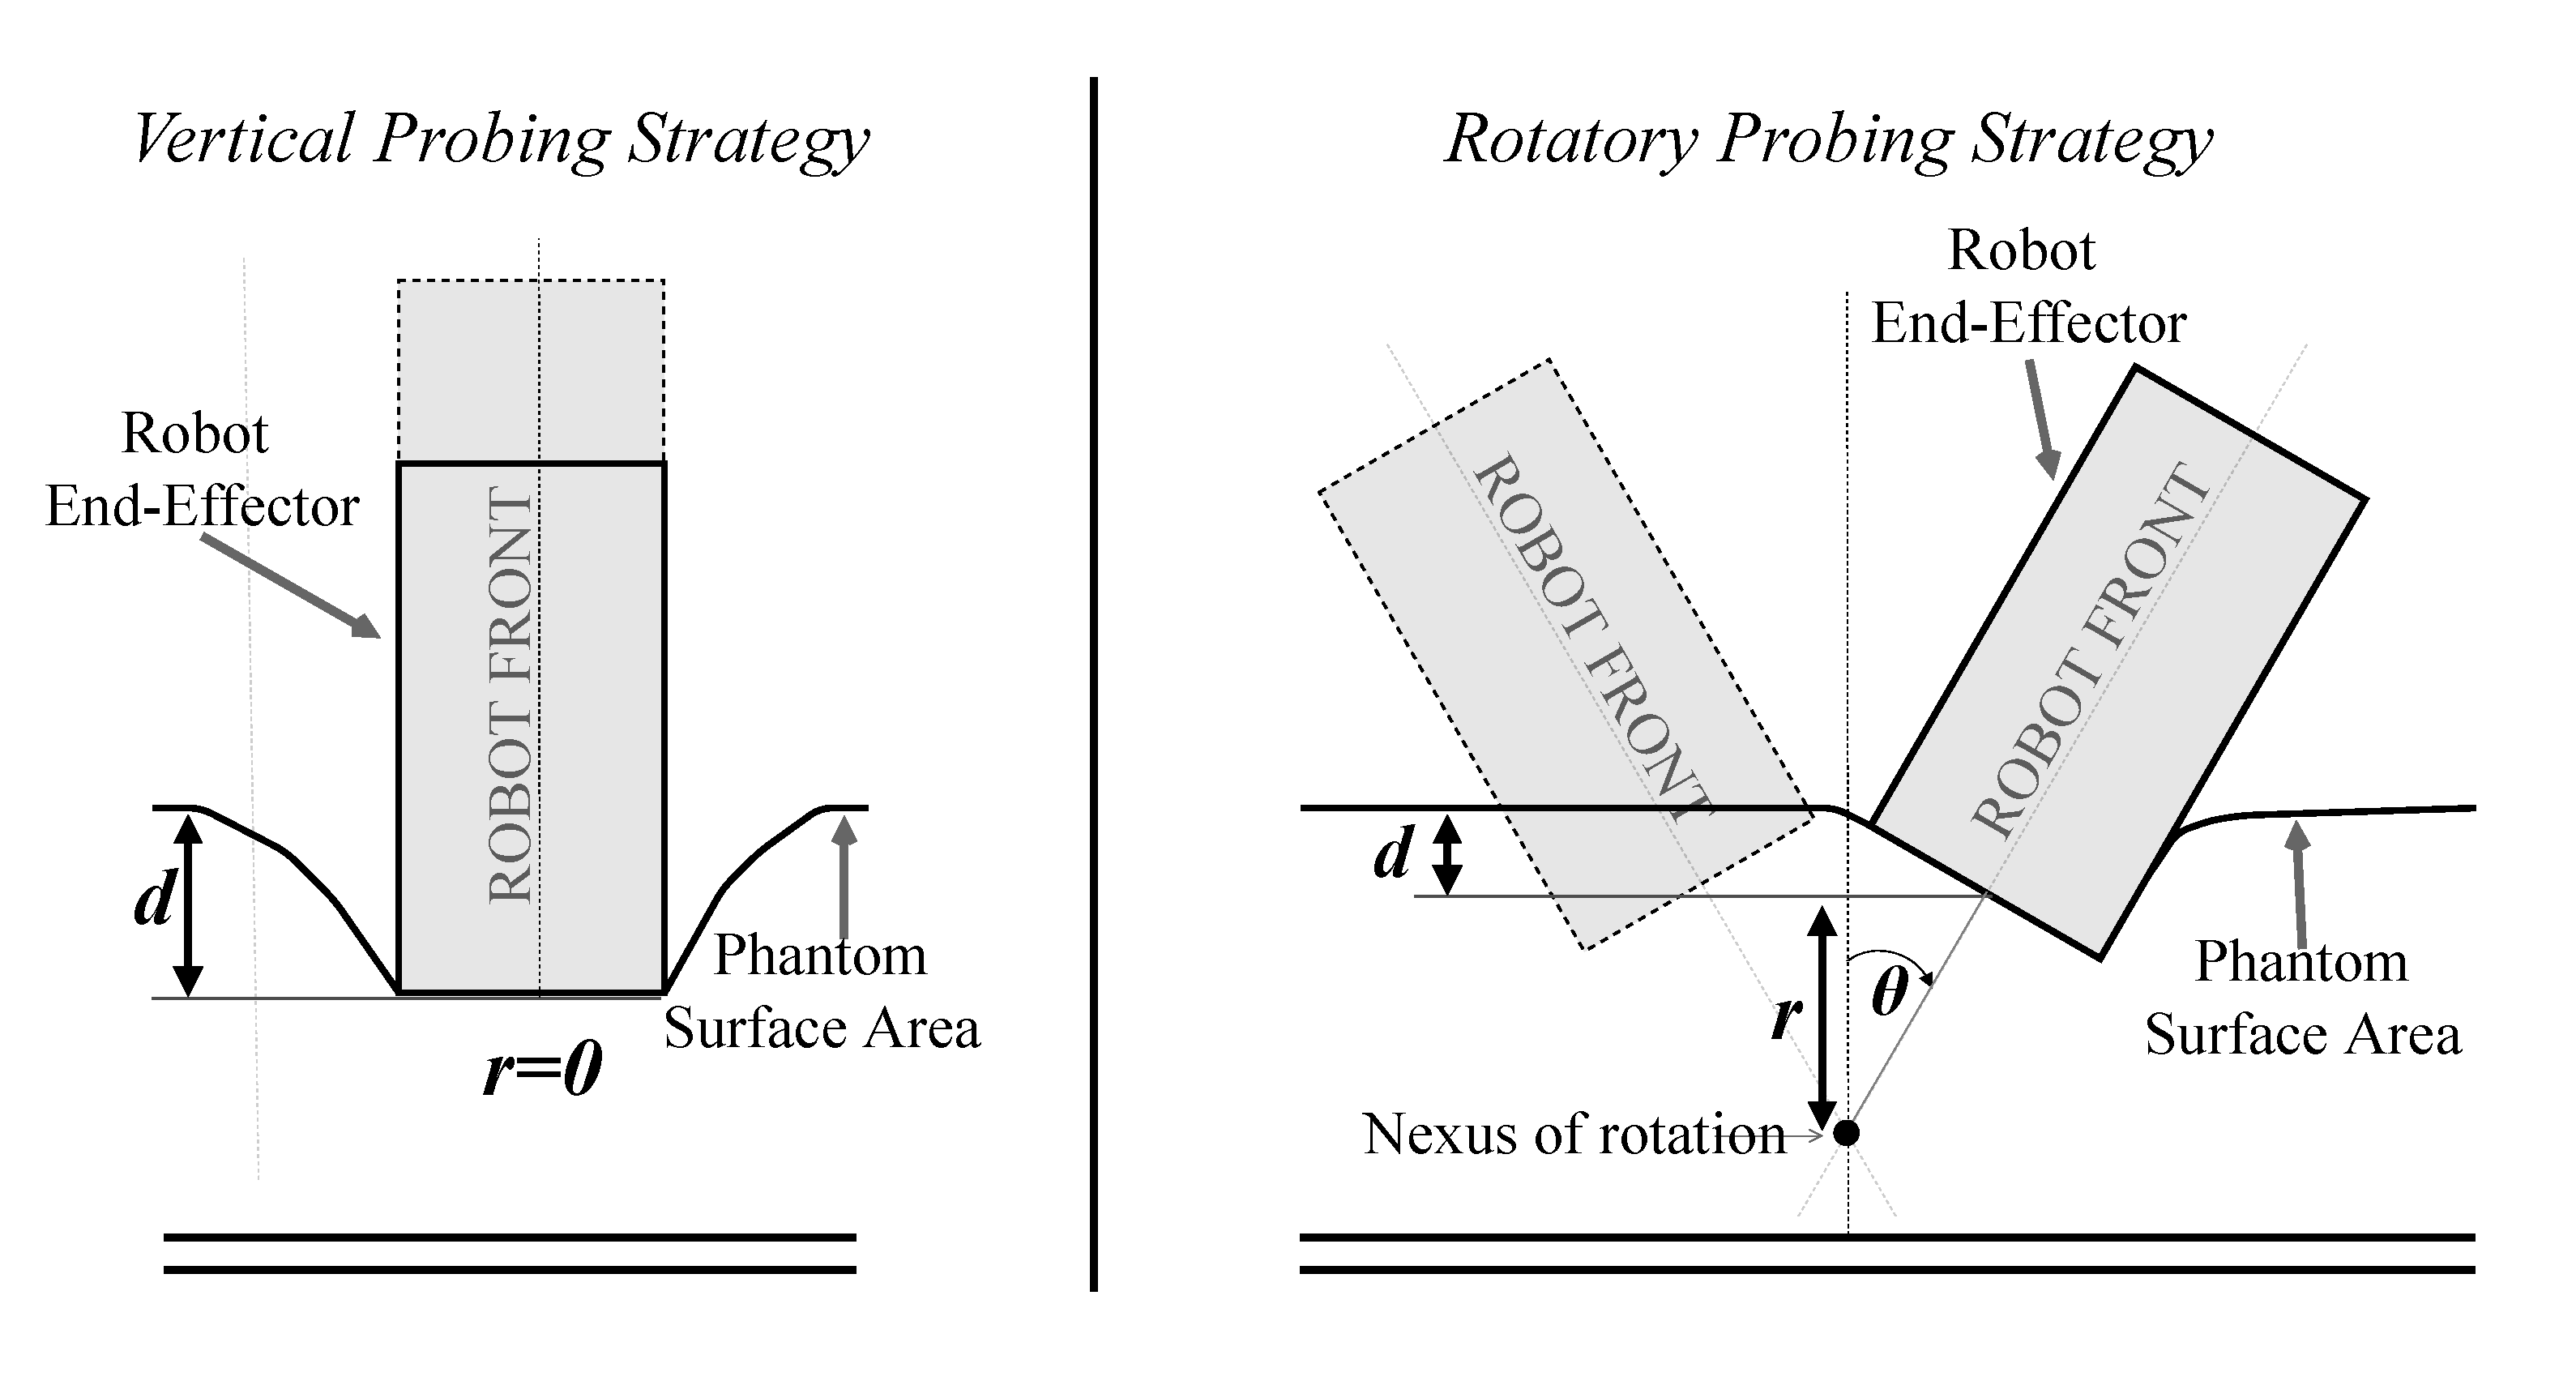
\includegraphics[width=\columnwidth]{./figs/motion_diagram.pdf}
	\caption{\color{red}{Diagram of the two probing motions employed. The vertical probing motion is performed when $r=0$ and is described by the parameter $d$. The rotatory motion is performed with $r>0$, and is fully described by both the $d$ and $r$ parameters.}}
	\label{probing}
\end{figure}


\section{Analytical Framework} \label{sec_th_framework}
\color{red}
%In order to investigate the hypothesis 
In this paper we consider the framework in Fig. \ref{conceptual_map}. In the framework, an agent retrieves tactile sensor information while interacting with samples of objects, defined by a task. Here, the tactile information is directly influenced by the interactions with the samples. A categorization system allows for the information to be: first, re-encoded into a meaningful, lower-dimensional space (Cognitive Mapping); second, differentiated into useful categories (Category Formation). The abstraction level corresponds to the number of categories that should be observed in the sensor information and has a direct influence on the significance of the formed categories. 
At its limit, 2 categories might be too coarse to be useful in capturing differences amongst different types of objects, while a number of categories equal to the number of object samples is impractical in identifying any similarities amongst them, and therefore amongst similar objects. The direct influence of the physical interactions to the tactile information, if substantial, should be observable in the category formation process. 
%Moreover, the framework captures the relationship between the response of the 
%tactile sensor, already influenced by motion, and the properties of the samples the agent interacts with. 

\begin{figure}[]
	\centering
	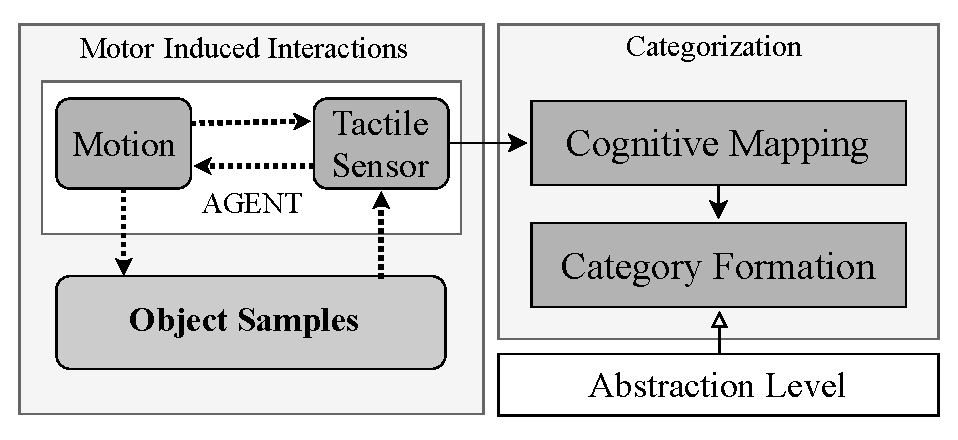
\includegraphics[width=\columnwidth]{./figs/conceptual_framework}
	\caption{Analytical Framework.}
	\label{conceptual_map}
\end{figure}

\subsection{Task and Physical Interactions}\label{sec_int}
Within the considered framework, the agent is an embodied system equipped with a tactile sensor, and capable of performing probing actions. The interactions consist of physical probing, through different strategies, of target areas in a soft phantom, as was described in Section \ref{sec_motor_interactions}.
\color{black}
As exemplified in Fig. \ref{self_org_processing}, an experiment consists of an agent probing a preselected phantom 
with a chosen probing strategy. The agent iteratively selects a target area in the phantom to probe, and performs 
the chosen probing strategy for the experiment (described by $\Theta$) while acquiring and storing tactile 
information. After probing all intended areas the stored sensor information can undergo categorization.

\subsection{Categorization}\label{sec_categorization}

\begin{figure*}[]
	\centering
	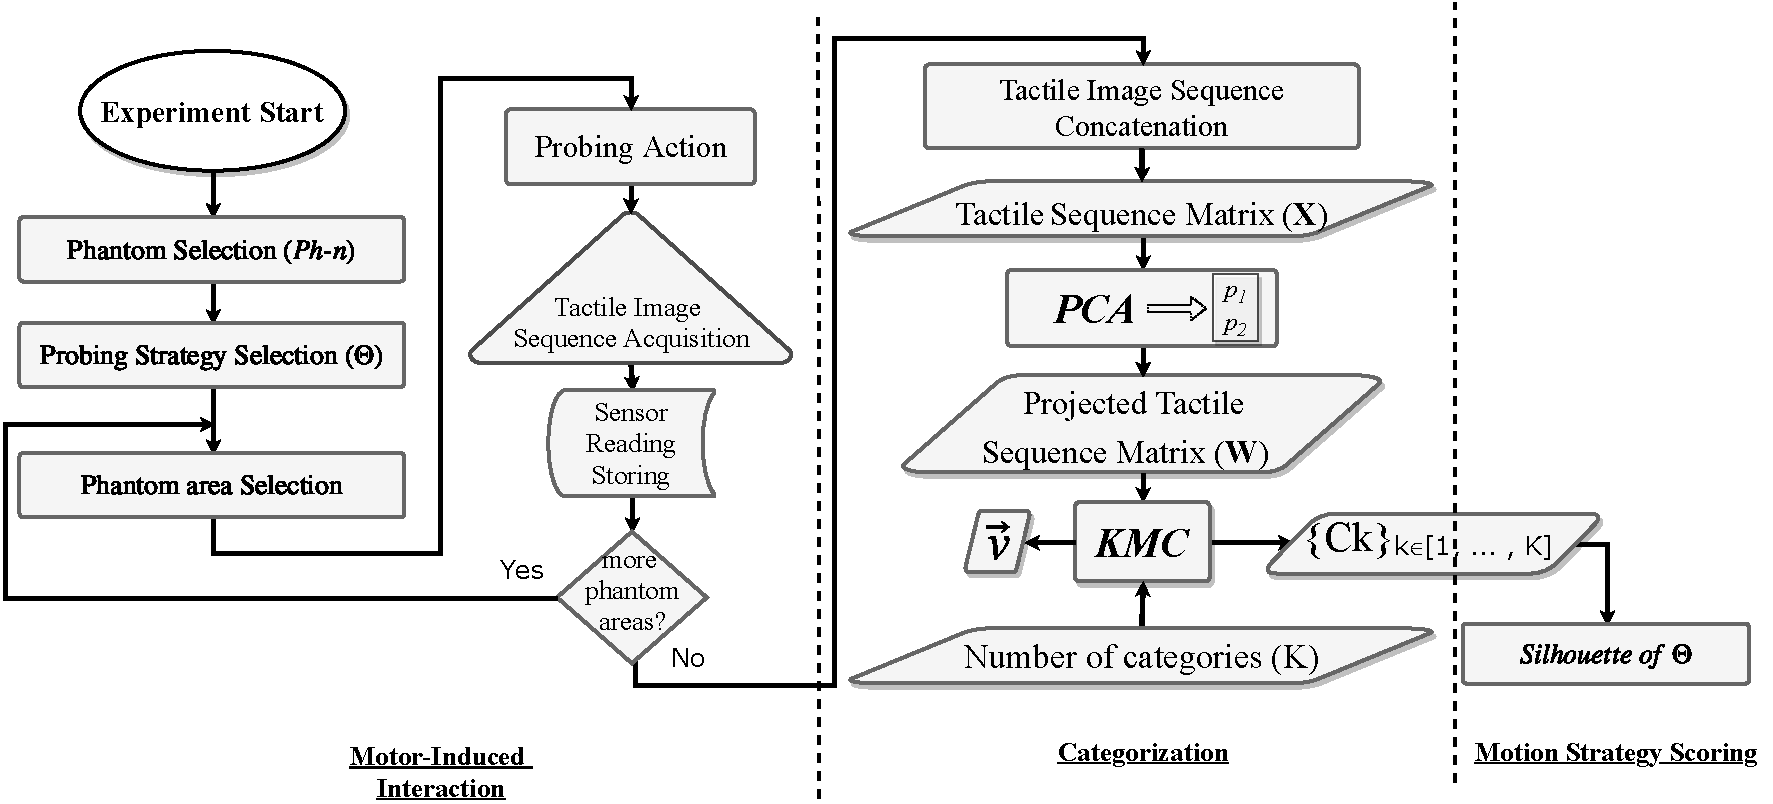
\includegraphics[width=.8\textwidth]{./figs/motion_primitive_preprocessing.pdf}
	\caption{Implementation steps of the Theoretical Framework.} %{After acquiring morphologically processed $tactile\ images$ for each object in a set, the high dimensional images are first projected in a 2-dimensional subspace ($PCA$) and finally clustered in an unsupervised manner through the $KMC$ algorithm. After clustering, $v$ is vector containing the cluster membership of each object in the initial set.}%}
	\label{self_org_processing}
\end{figure*}

\subsubsection{Cognitive Mapping}\label{sec_dim_reduction}

A process is needed to reduce the high dimensionality of the spatiotemporal data acquired through the 
tactile sensor, while interacting with the environment. We define a tactile image sequence as a series 
of tactile sensor readings taken at set intervals, and concatenated into a single array. After acquiring 
tactile image sequences for each probed location, we use Principal Component Analysis projection ($PCA$) 
\cite{tipping_probabilistic_1999} to reduce the dimensionality of the acquired data \cite{lloyd_least_1982}. 

For a set of $N$ different locations in a phantom, let $\mathbf{X}$ be a $(N\times D)$ matrix where each unique 
tactile image sequence for a probed location is a $D$ dimensional row ($D\gg2$) in the matrix. The dimension 
of $D$, then, will be strictly dependent on the probing strategy and on the interval at which the agent 
captures each tactile image within the sequence. 

After obtaining the tactile image sequences matrix $\mathbf{X}$, we begin the process by finding 
the average tactile sequence $\vec{\mu}$ as:
\begin{equation}
\vec{\mu} = \frac{1}{N}\sum_{i=1}^{n}\vec{x}_i
\end{equation}
where $\vec{x}_i$ is a column vector corresponding to the $i^{th}$ row in $\mathbf{X}$. We compute a 
($D\times D$) scatter matrix $\mathbf{S}$ as:
\begin{equation}
\mathbf{S} = \sum_{i=1}^{N}(\vec{x}_i-\vec{\mu})(\vec{x}_i-\vec{\mu})^T
\end{equation}

and use Single Value Decomposition to factorize $\mathbf{S}$ into
\begin{equation} \label{eq_SVD}
\mathbf{S} = \mathbf{Q}\mathbf{\Lambda} \mathbf{Q}^{-1}
\end{equation}
\noindent where $\mathbf{Q}$ is a matrix such that each column $q_j$ corresponds to an eigenvector 
of $\mathbf{S}$, and each element $\lambda_{jj}$ in the diagonal matrix $\Lambda$ is its corresponding 
eigenvalue. We list the eigenvectors in ascending order of eigenvalue and select the first two in the list. 
Let $\vec{p}_1$ and $\vec{p}_2$ be the selected eigenvectors obtained from $PCA$. 

We form a $(D\times 2)$ projection matrix $\mathbf{P}$ as:
\begin{equation}
\mathbf{P}=\begin{bmatrix}\vec{p}_1^{\ T}, \vec{p}_2^{\ T}\end{bmatrix}	
\end{equation}
where $\vec{p}_1^{\ T}$ and $\vec{p}_2^{\ T}$ are column vectors in $\mathbf{P}$. 

Finally, we project the $D$-dimensional row vectors in $\mathbf{X}$ onto a 2-dimensional subspace by:
\begin{equation}
\mathbf{W}=\mathbf{X}\cdot \mathbf{P}
\end{equation}
where $\mathbf{W}$ is a $(N\times 2)$ matrix. Each row in the matrix is a 2-dimensional $encoding$ of a 
tactile image sequence for a probed location.


\begin{figure*}[]
	\centering
	\begin{subfigure}[b]{.12\textwidth}
		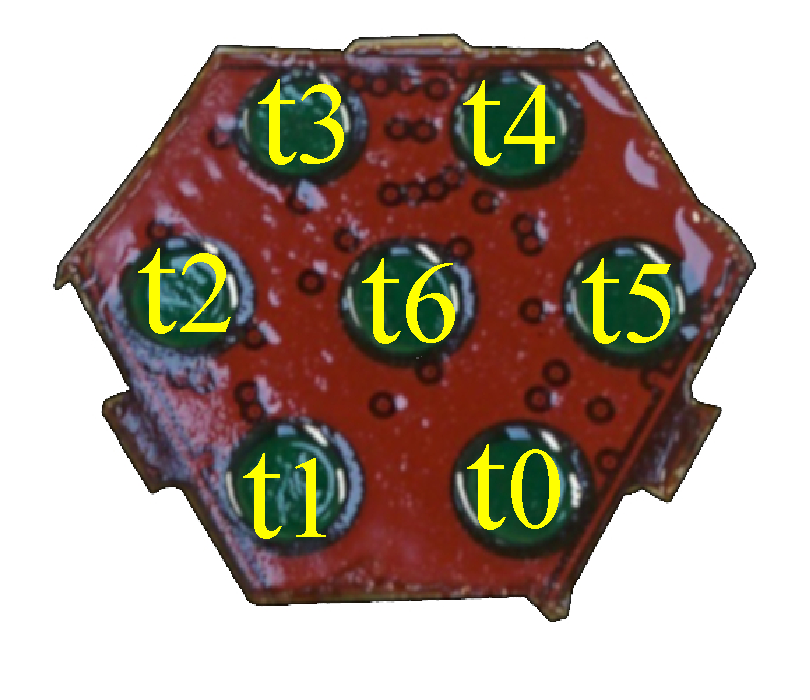
\includegraphics[width=\textwidth]{./figs/skin.pdf}
		\vspace{1pt}
		\caption{}
		\vspace{6pt}
		\label{rawnabs:skin}
	\end{subfigure}
	\hspace{0.005\textwidth}
	\begin{subfigure}[b]{.38\textwidth}
		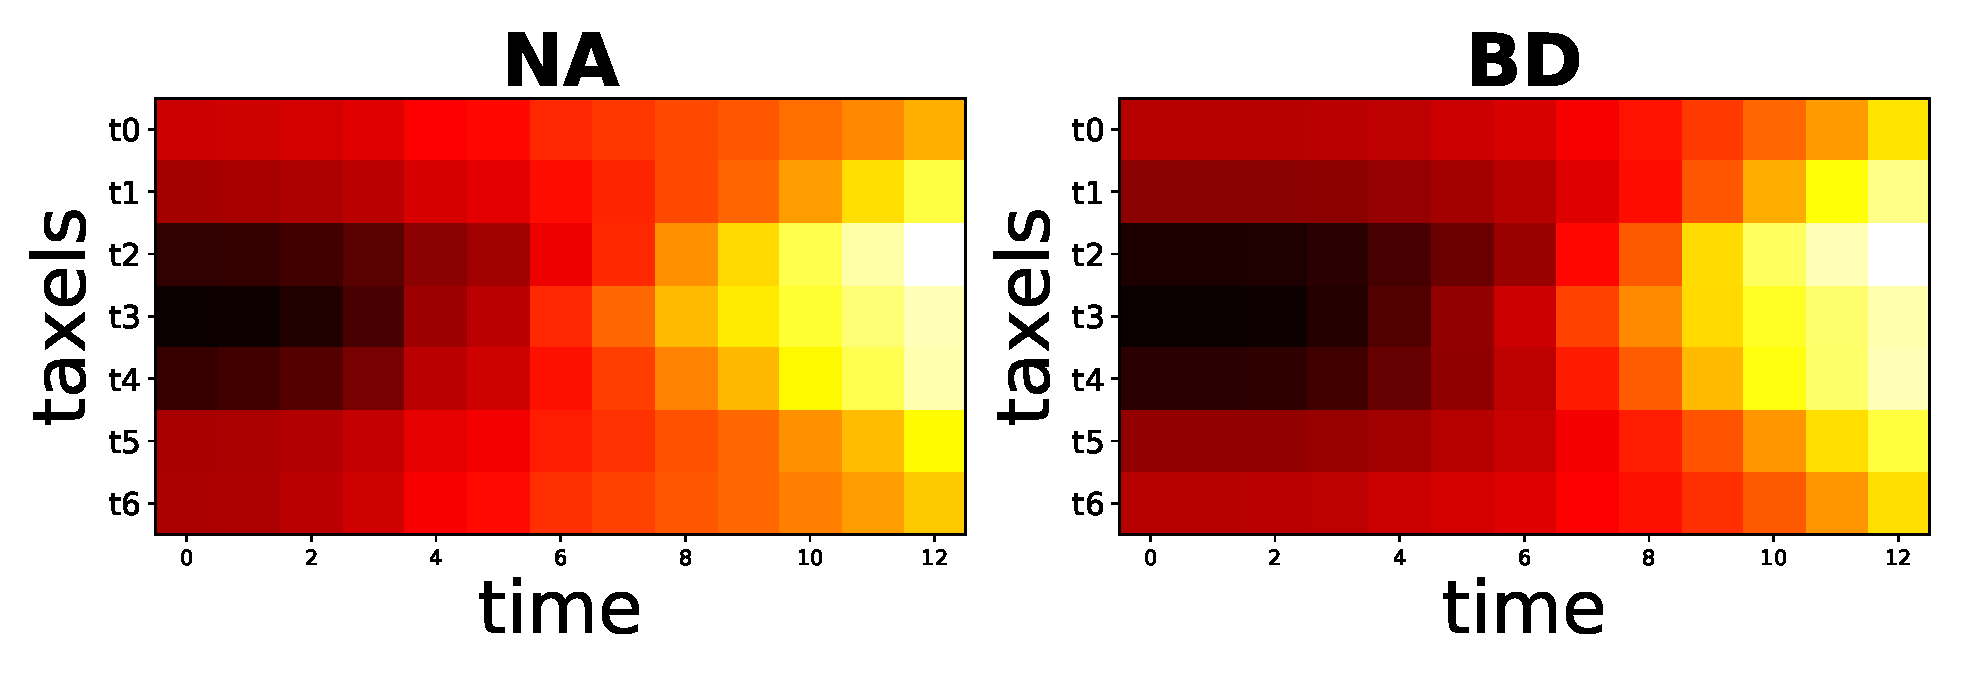
\includegraphics[width=\textwidth]{./figs/phantom1properties_rawdataf_Vertical-d6_5.eps}
		\caption{$\Theta = \small{\begin{Bmatrix}6.5\\ 0\end{Bmatrix}}$}
		\label{rawnabs:d6_5}
	\end{subfigure}
	\hspace{0.005\textwidth}
	\begin{subfigure}[b]{.38\textwidth}
		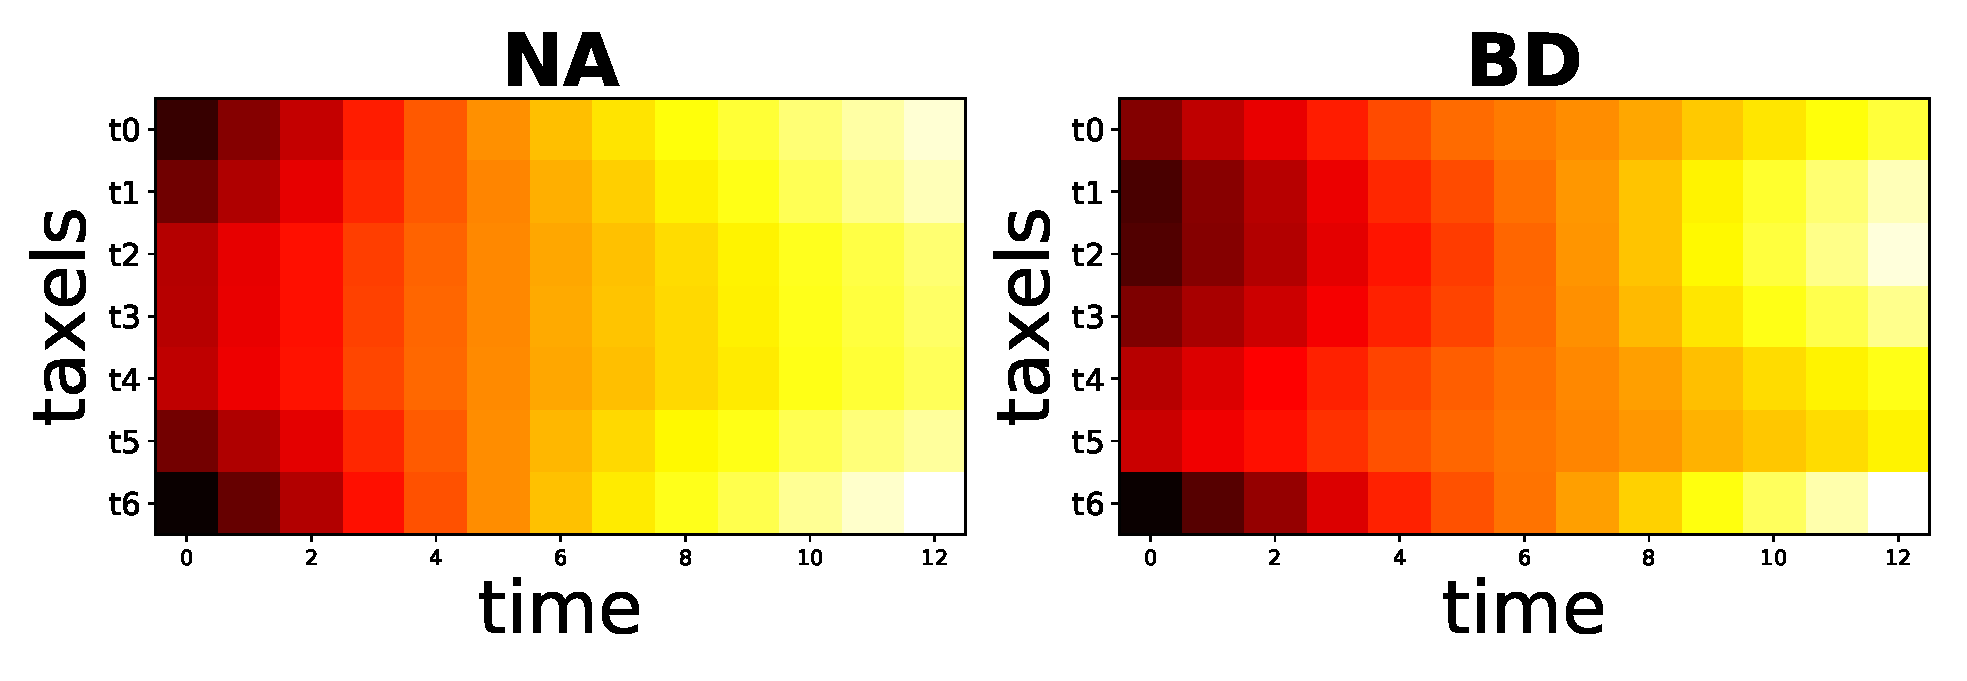
\includegraphics[width=\textwidth]{./figs/phantom1properties_rawdataf_Vertical-d19_5.eps}
		\caption{$\Theta = \small{\begin{Bmatrix}19.5\\ 0\end{Bmatrix}}$}
		\label{rawnabs:d19_5}
	\end{subfigure}
	\caption{\color{red}{Raw spatiotemporal tactile image sequences, as captured when probing $Ph\text{-}2$ vertically at varying depths, in an area containing no hand inclusion, and an area containing a $15mm$ inclusion placed $20mm$ deep. Figure (a) shows the spatial layout of the taxels in the Cyskin sensor, while each tactile image sequence in (b) and (c) corresponds to a re-shaped $x_i$. }}
	\label{rawnabs}
\end{figure*}

\subsubsection{Category Formation and Abstraction Level}\label{sec_clustering}
To observe the effects of the probing strategies to the tactile sensor information we wish to have a process to 
categorize the re-encoded sensor information. We use K-Means Clustering ($KMC$) to find clusters in the data, 
where each found cluster will represent a potential category of inclusion types. The abstraction level is set by the
number of clusters we wish to find in the data. 
%The category represented by each cluster will be different depending on how coarsely or finely the agent wishes to 
%see the probed areas. 
We initialize the $KMC$ algorithm with random centroids, and split the re-encoded sequences in $\mathbf{W}$ into $K$ 
clusters by:
\begin{equation}
\vec{v} = KMC_{K}(\mathbf{W})
\end{equation}
The resulting $\vec{v}$ is an N-dimensional array, where each element $\vec{v}_i\in\{1, ..., K\}$, 
and $\forall i\in \{1,\ ...\ , N\}\ \exists j\in \{1,\ ...\ , N\}:\ i\neq j\ \land\ v_i\neq v_j$ 
(Fig. \ref{self_org_processing}); in other words, none of the resulting clusters can contain all the sample 
areas in the phantom. 

In general $\vec{v}_i=k$ only if the $i^{th}$ tactile image sequence belongs to cluster $k$, thus the $\vec{v}$ 
vector contains the cluster membership of each probed location in the initial set. 

To avoid cluster anomalies due to the random centroid initializations we run the $KMC$ algorithm three times 
and discard the clustering attempt if, after convergence, any of the three cluster guess vectors differs from 
any other. At the end of the clustering process a list of centroids $C$ is obtained, uniquely dividing the 
space into K categories (\ref{self_org_processing}). In this context, the cluster assignments for each probed 
location is largely dependent on the probing strategy employed. 
%The change in cluster assignment is the main object of analysis in the following sections.

\color{red}
\subsection{Motion Strategy Scoring} \label{sec_sil_coeff}
At the end of the clustering process it is necessary to be able to assess the usefulness of the probing in generating meaningful data for classification. For the unsupervised clustering algorithm to be able to find meaningful clusters in the re-encoded tactile data, it is necessary that the data exhibits structure. Therefore we score the probing strategy that generated the data via a metric of structure tightly connected to the type of clustering utilized in this paper, i.e. the silhouette score \cite{rousseeuw1987silhouettes}. 

The silhouette score $s(i)$ for cluster $i$ can be computed as:
\begin{equation}
s(i) = \frac{b(i)-a(i)}{\operatorname{max} (a(i),\ b(i))}
\end{equation}
where $a(i)$ is the mean intra-cluster distance of cluster $i$, and $b(i)$ is its mean nearest-cluster distance. 
We will refer to the silhouette score $s$ as the average score for each cluster found by KMC, i.e.: 
\begin{equation}
s = \frac{\sum_{i=1}^{K} s(i)}{K}
\end{equation}
The score will thus be a number $s \in [-1,1]$, where data exhibiting more structure will score higher $s$ values. 

After probing the selected phantom through various probing strategies, the maximum observed silhouette score can identify which probing strategy is capable of generating structured data for hard inclusion detection and classification. The analysis as described thus far can be done without any prior labelling. After, a supervised method can, for example, be used to perform the classification. 


\color{black}
\subsection{Experimental Procedure} \label{sec_overall_approach}
%( 16*5 )*2
We execute 180 experiments, each of which sees the robot probing all 16 areas of $Ph\text{-}1$ or $Ph\text{-}2$ with the 
preferred $\Theta$ parameters. The experiments are carried out for all combinations of $d\in[6.5mm, ... , 20.5mm]$ at $1mm$
increments and $r\in[0mm, 10mm, 12mm, 14mm, 16mm]$. The bounds were chosen to reach the minimal/maximal experimentally 
feasible probing depth and rotation with the robotic arm, and the devised soft phantoms. 

For each of the experiments, after the probing has ended, the time-concatenated data is used to form the tactile 
image sequence matrix described (see Section \ref{sec_dim_reduction}). The matrix can then be used to re-encode the
tactile sensor information for each probed location into a lower dimensional space ($Cognitive\ Mapping$). After clustering, each probed location will be differentiated into one of a predetermined number of categories ($Category\ Formation$).


\section{Results} \label{sec_results}
The following sections will progressively analyze the described framework, starting from the dimensionality reduction
process ($PCA$), to the repercussions of physical interactions to categorization ($KMC$).


\subsection{Sound Dimensionality Reduction}

One of the principal components of the proposed framework is the reduction of the high dimensional 
spatiotemporal tactile information, into re-encoded lower dimensional data. An example of the 
acquired tactile information is shown in Fig. \ref{rawnabs}.
%For each experiment, the $\mathbf{X}$ matrix at most contains $N$ $D$-dimensional tactile image 
%sequence vectors, corresponding to the $N$ locations of the phantom to probe, and where $N=16$ 
%and $72\ge D \ge420$, depending on the probing strategy. The data then, will at most live in an $N$ 
%dimensional subspace of $D$.  
Without knowing which category each tactile sequence vector $\vec{x_i}$ belongs to, it is impossible to assess
the quality of dimensionality reduction from $\mathbf{X}$ to $\mathbf{W}$. However, it is feasible to maximize the
information retention in the original tactile sensor data.

\begin{figure*}[]
	\centering
	\begin{subfigure}[b]{.47\textwidth}
		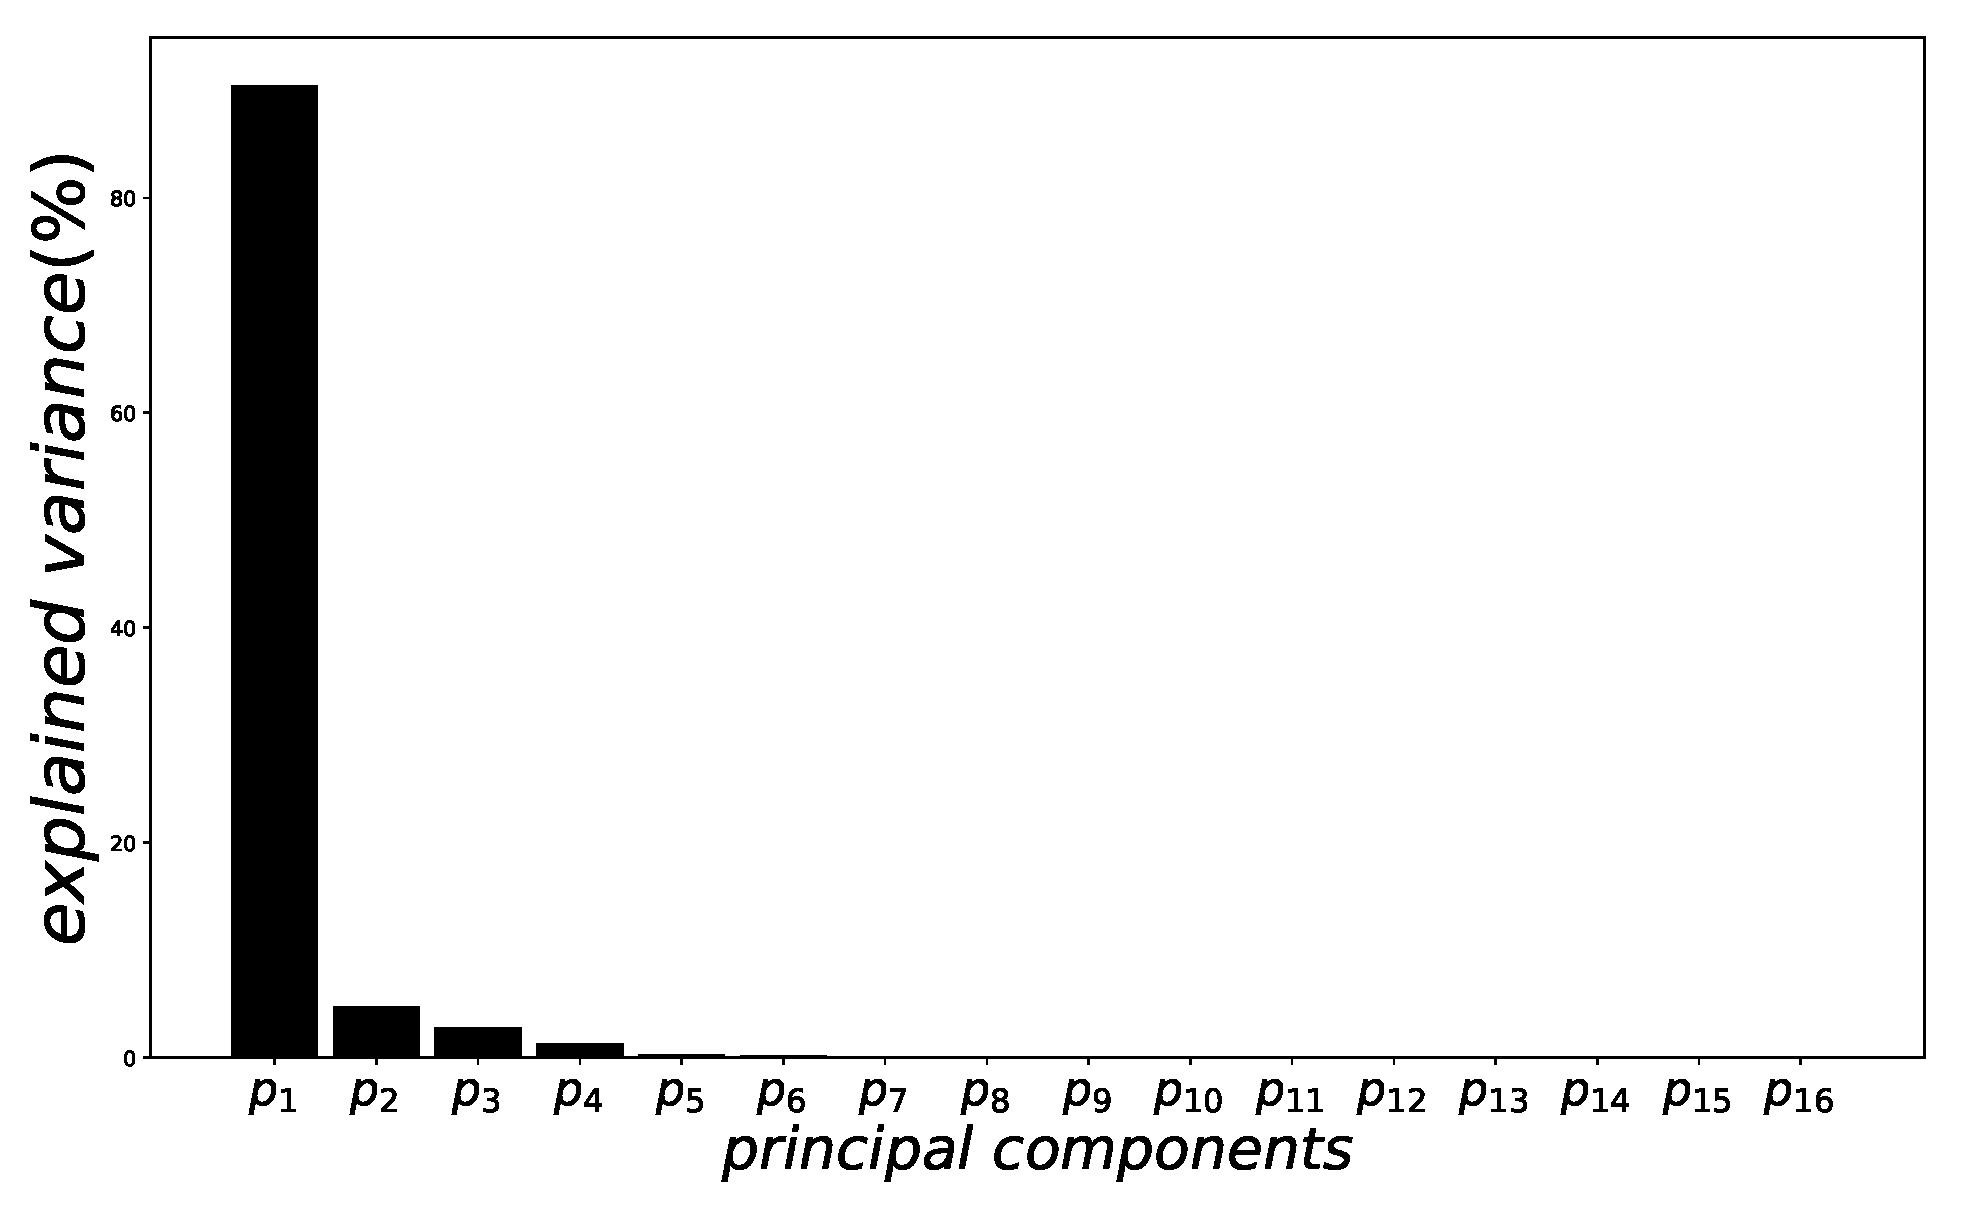
\includegraphics[width=\textwidth]{./figs/phantom2properties_pcafig_Vertical-d14_5.eps}
		\caption{$\Theta = \small{\begin{Bmatrix}14.5\\ 0\end{Bmatrix}}$, $N=16$}
		\label{hist:1}
	\end{subfigure}
	\hspace{0.01\textwidth}
	\begin{subfigure}[b]{.47\textwidth}
		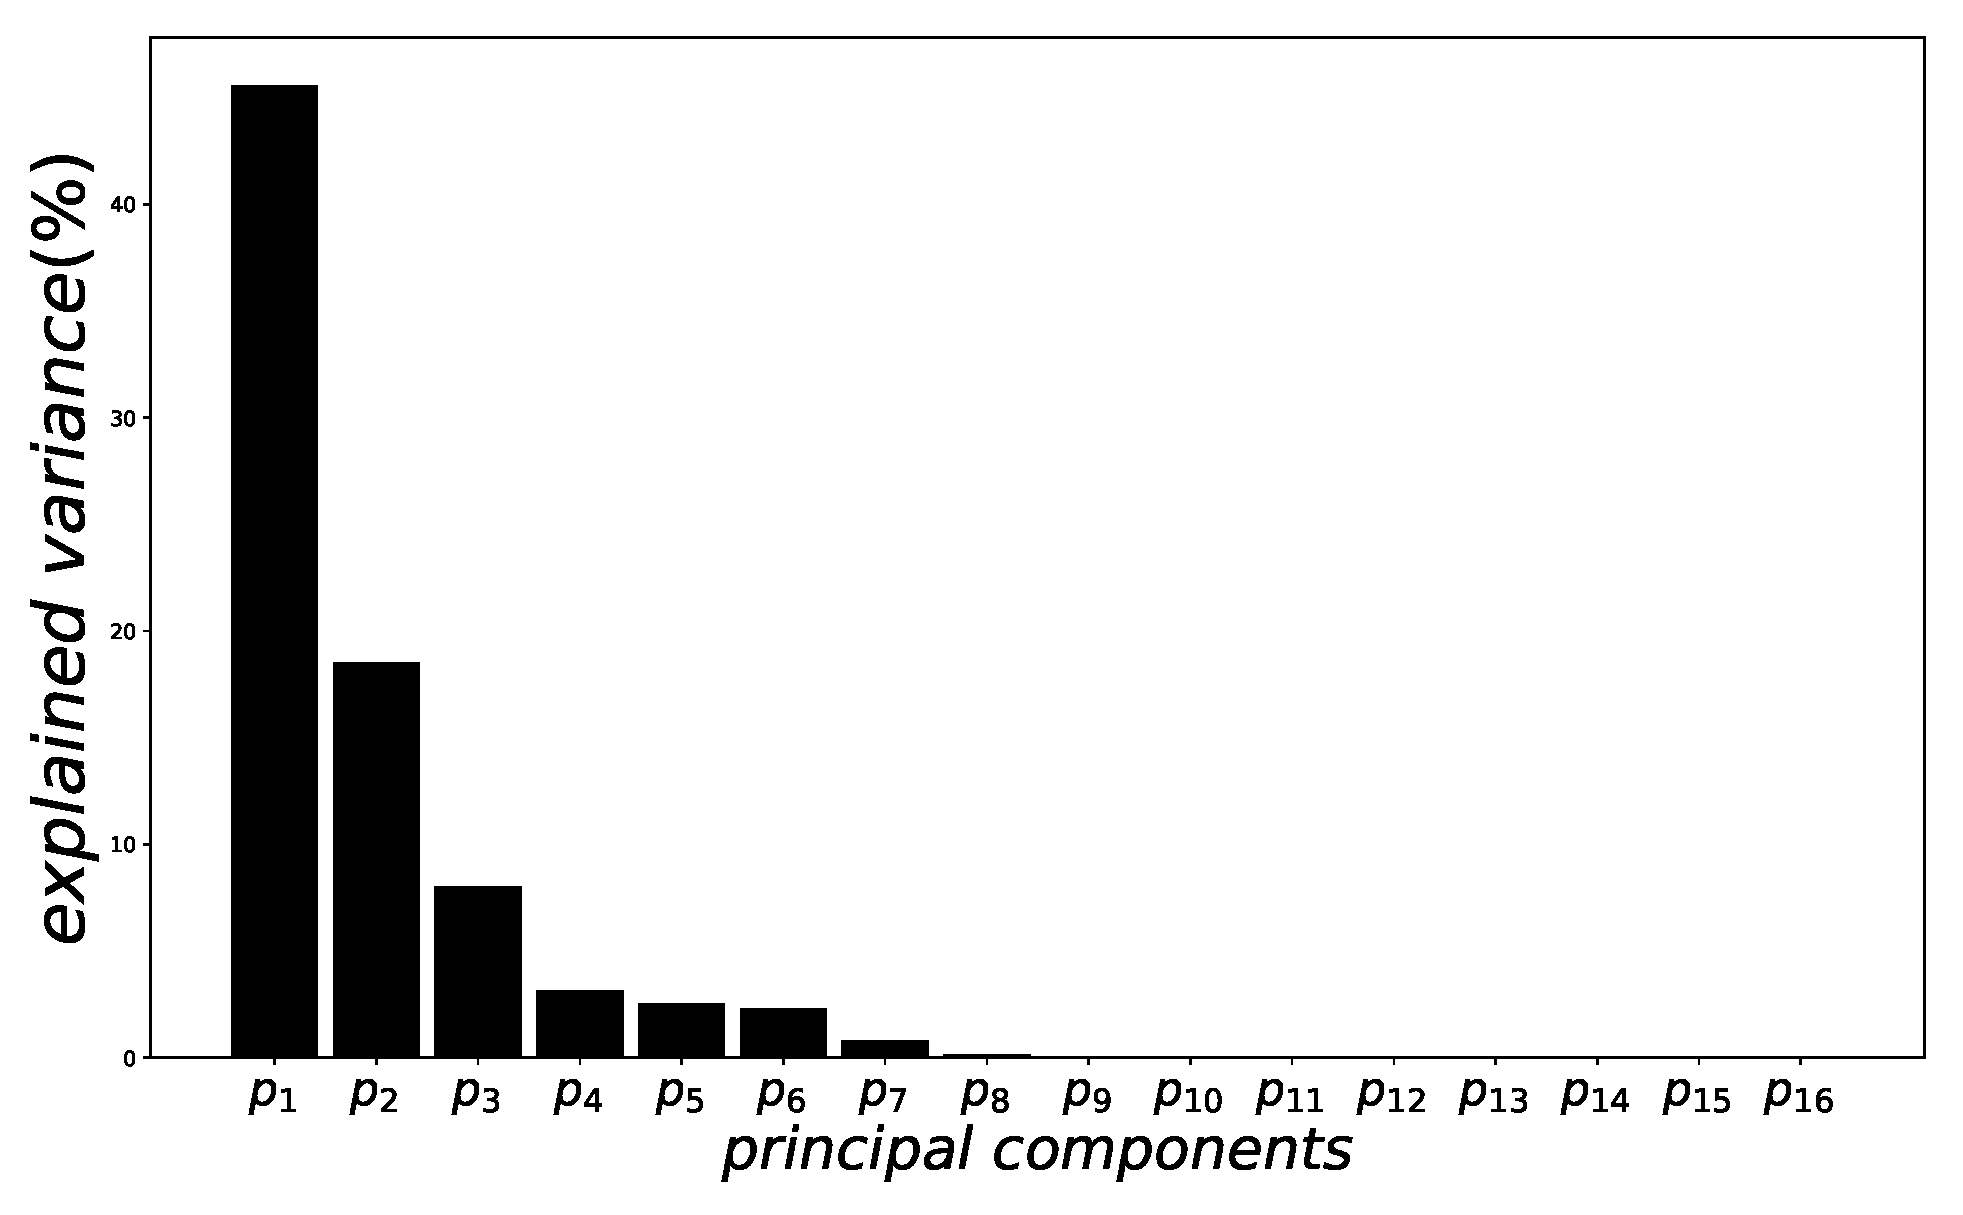
\includegraphics[width=\textwidth]{./figs/phantom2properties3-12-13-21-42-24-31-31-2_pcafig_Rotate-d190-r120.eps}
		\caption{$\Theta = \small{\begin{Bmatrix}18.5\\ 12\end{Bmatrix}}$, $N=8$}
		\label{hist:2}
	\end{subfigure}
	\caption[]{The explained variance of each principal component when projecting the $\mathbf{X}$ 
		matrix belonging to two different experiments where both the number of probed areas in $Ph\text{-}2$, to base the $PCA$ projection on, and the $\Theta$ parameters where changed.}
	\label{hist}
\end{figure*}
\begin{figure*}[]
\centering
\begin{subfigure}[b]{.48\textwidth}
	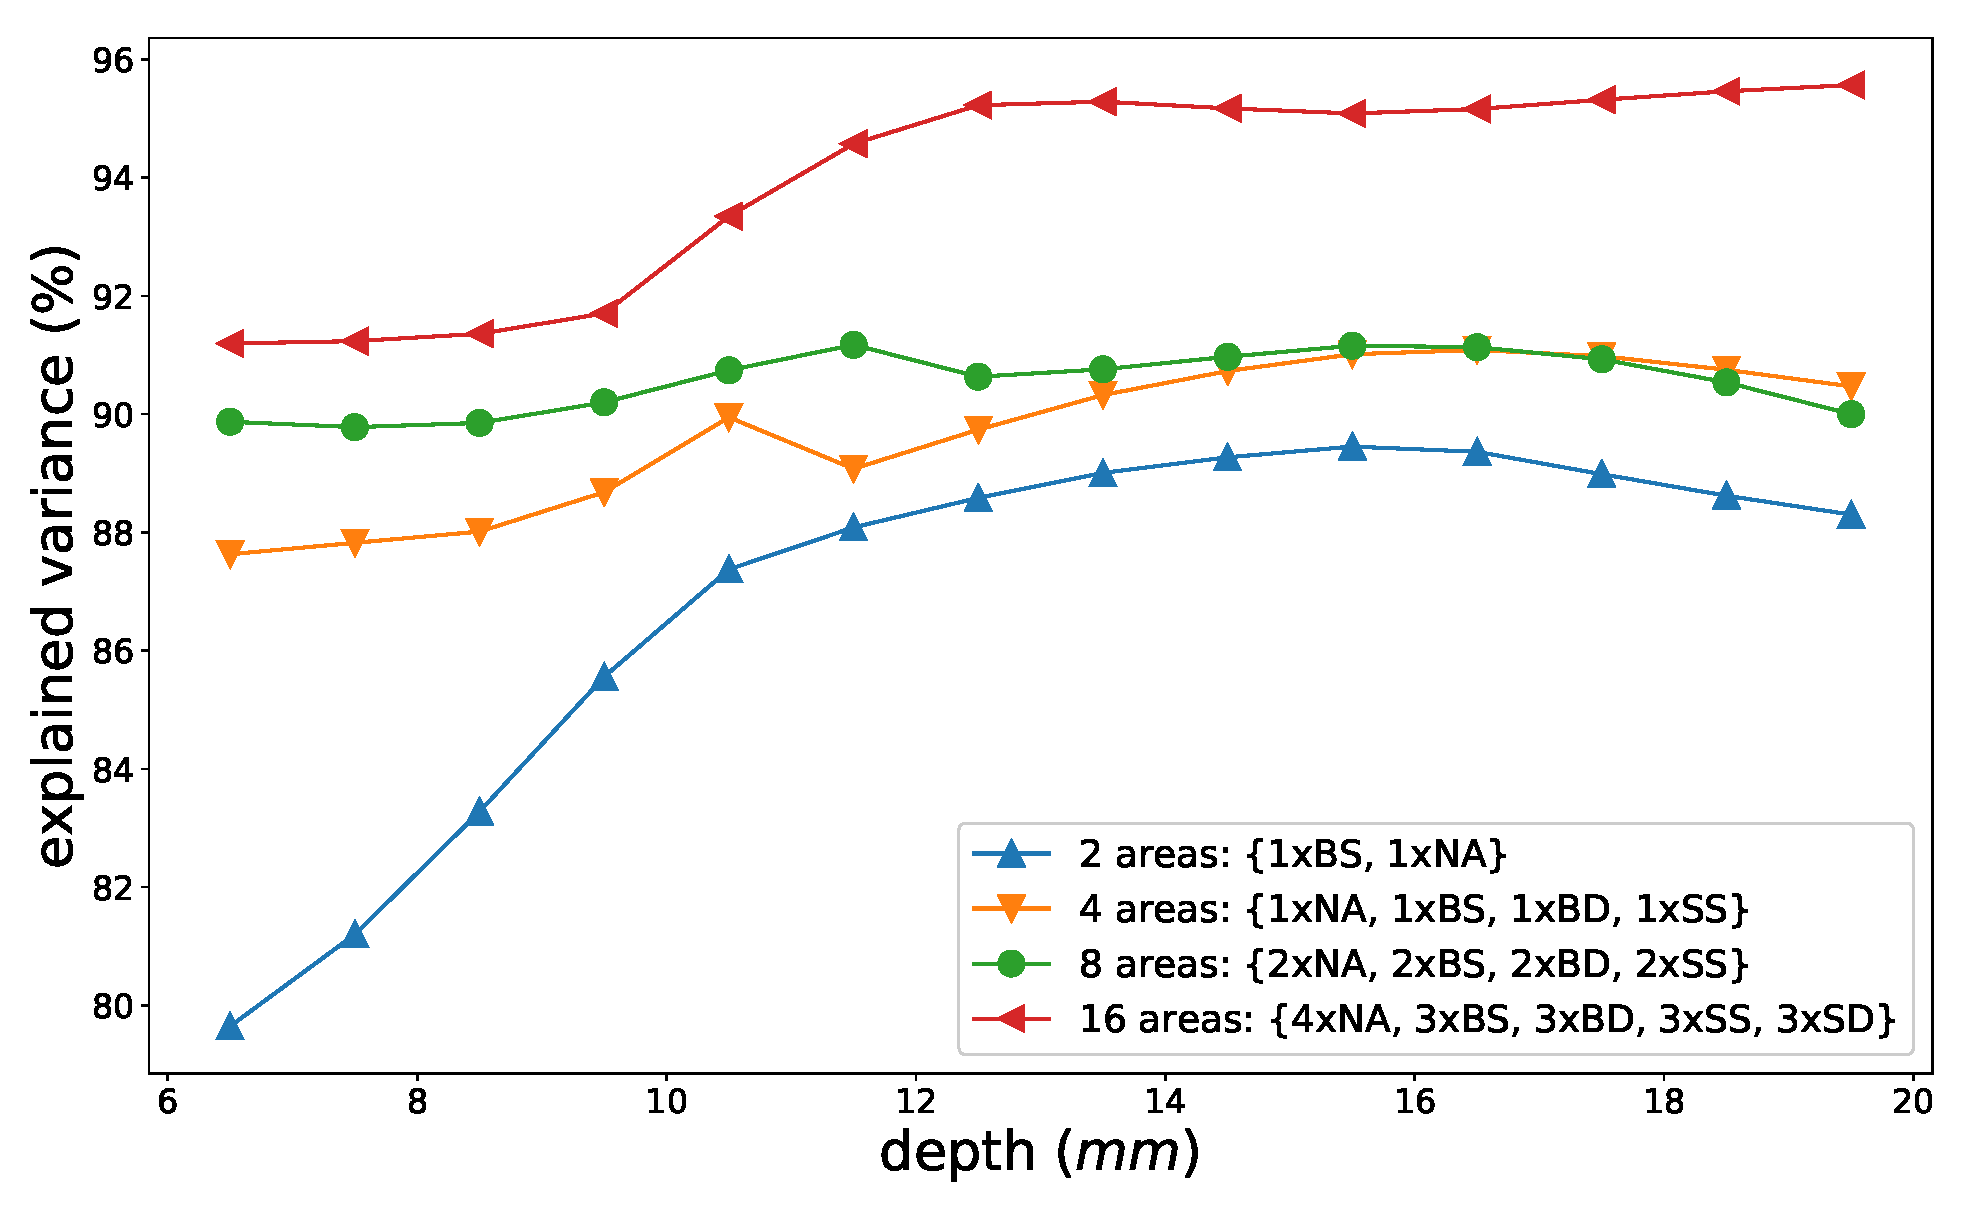
\includegraphics[width=\textwidth]{./figs/explained_variance_vertical_quantity.eps}
	\caption{$Ph\text{-}2$: Vertical Probing}
	\label{inf_retention_quantity:vertical}
\end{subfigure}
\begin{subfigure}[b]{.48\textwidth}
	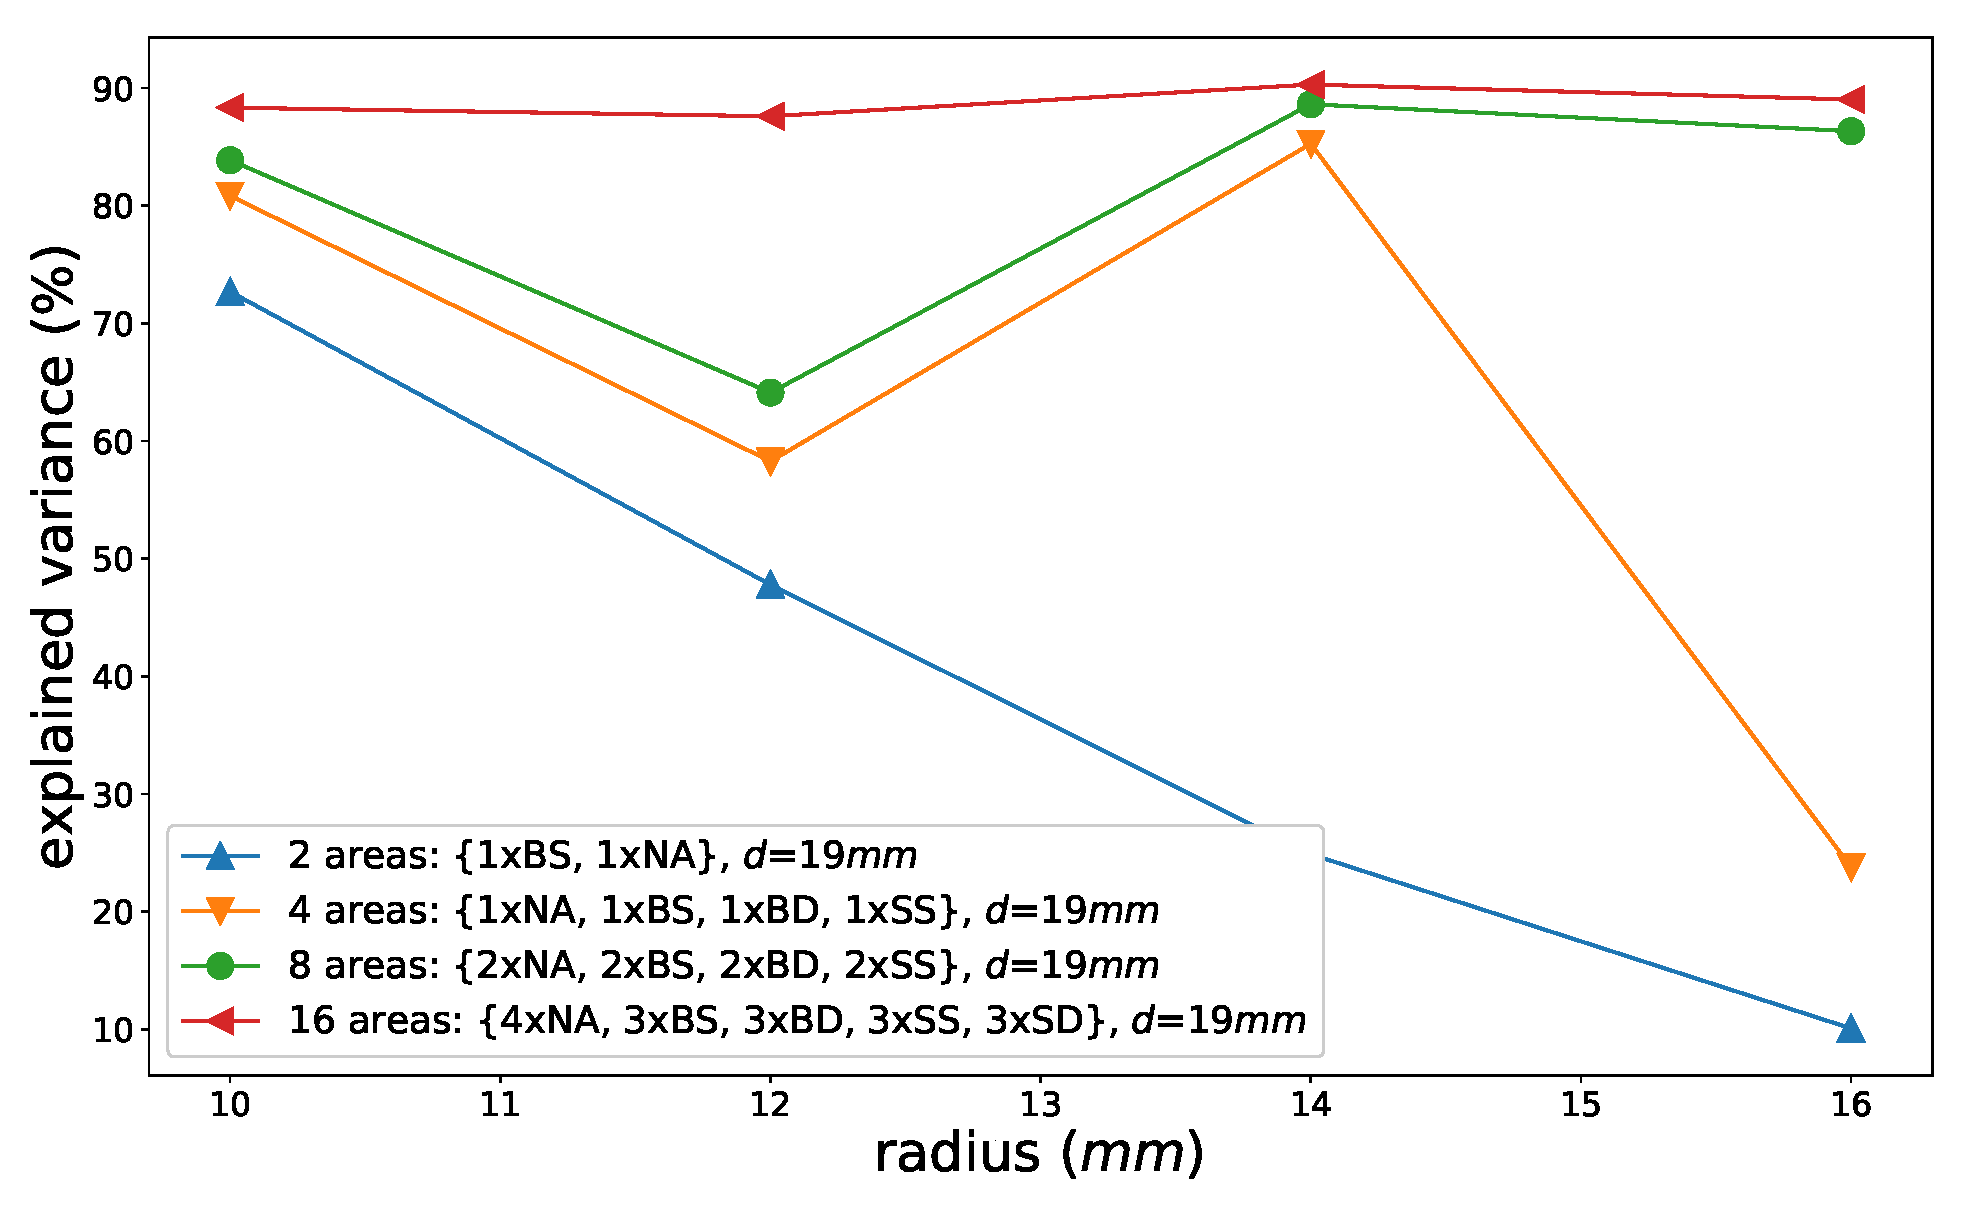
\includegraphics[width=\textwidth]{./figs/explained_variance_rotation_quantity.eps}
	\caption{$Ph\text{-}2$: Rotational Probing}
	\label{inf_retention_quantity:rotation}
\end{subfigure}
\caption{The change in explained variance by the 2D PCA subspace projection, when 
	probing vertically (a) and through the rotatory motion (b), changing the number of samples used 
	to find the principal components ($N$ in $\mathbf{X}$, see Section \ref{sec_clustering}). }
\label{inf_retention_quantity}
\end{figure*}

\begin{figure*}[]
\centering
\begin{subfigure}[b]{\columnwidth}
	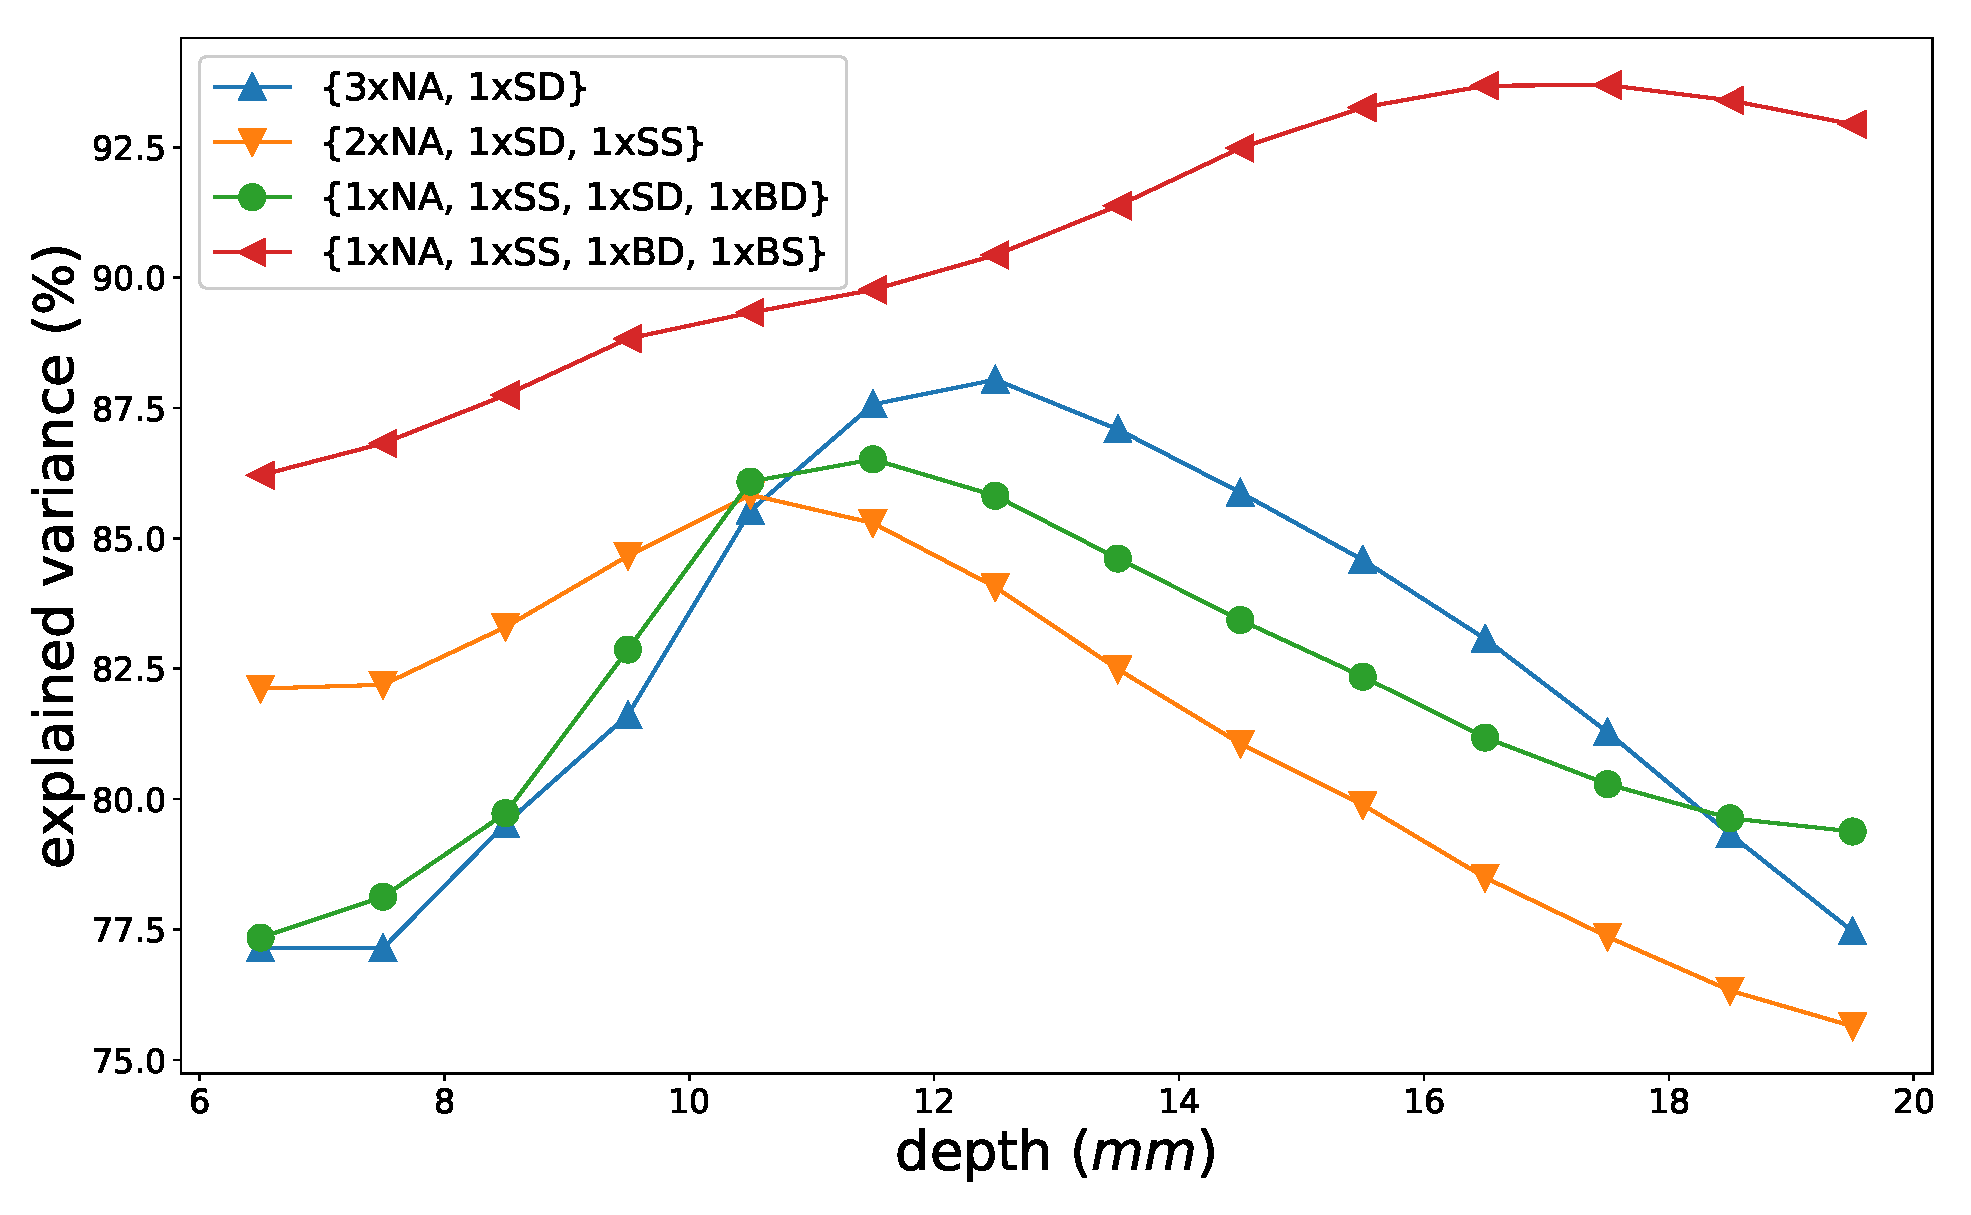
\includegraphics[width=\columnwidth]{./figs/explained_variance_vertical_quality.eps}
	\caption{$Ph\text{-}2$: Vertical Probing}
	\label{inf_retention_quality:vertical}
\end{subfigure}
\begin{subfigure}[b]{\columnwidth}
	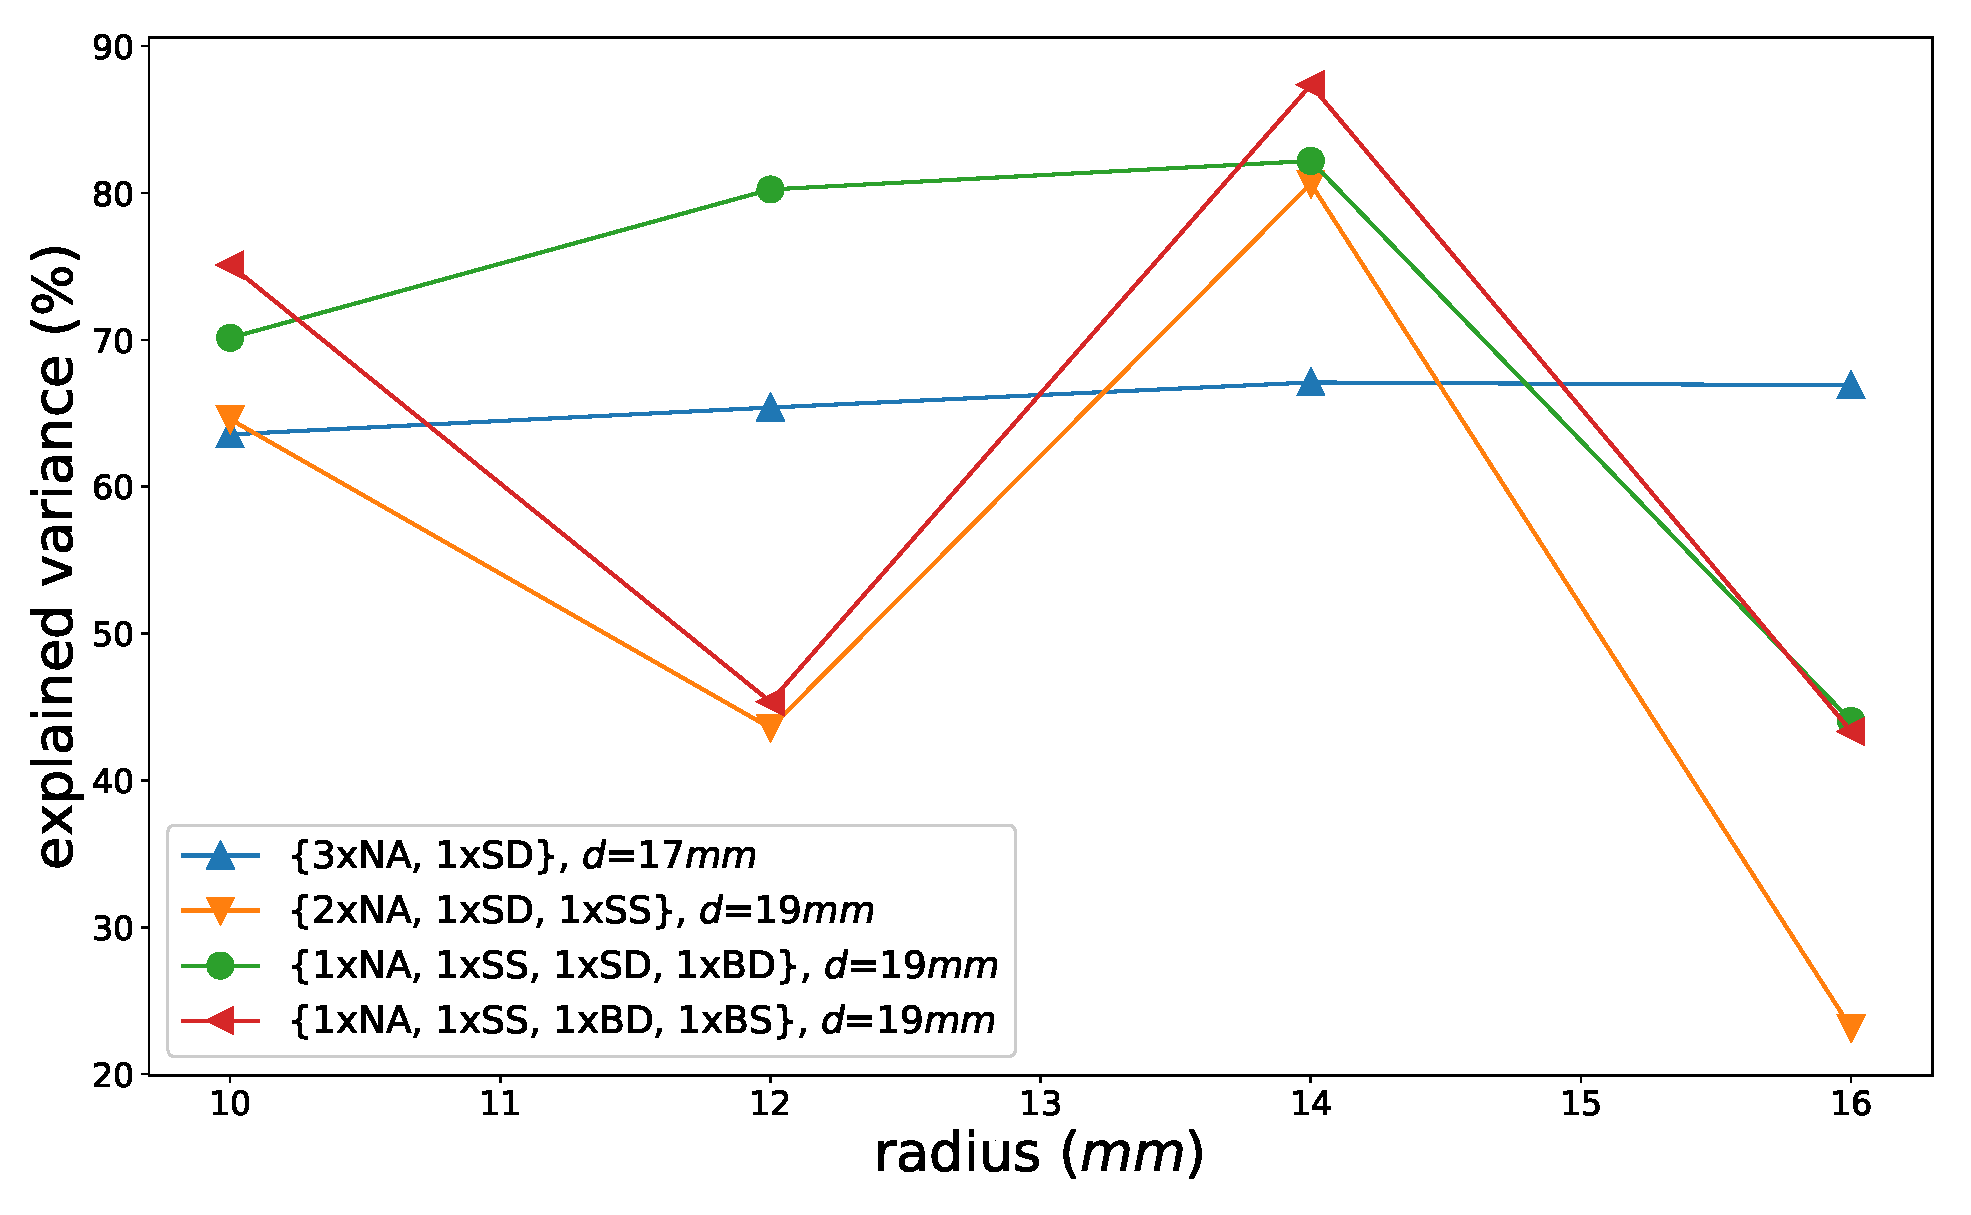
\includegraphics[width=\columnwidth]{./figs/explained_variance_rotation_quality.eps}
	\caption{$Ph\text{-}2$: Rotational Probing}
	\label{inf_retention_quality:Rotation}
\end{subfigure}
\caption{The change in explained variance by the 2D PCA subspace projection, 
	when probing vertically (a) and through the rotatory motion (b), changing the quality of 
	the samples used to find the principal components, while maintaining their number constant. }
\label{inf_retention_quality}
\end{figure*}

The explained variance can be thought of as a measure of the information captured by the PCA subspace after projection. 
As the eigenvalues in $\Lambda$ (see Eq. \ref{eq_SVD}) are proportional to the variance captured by the corresponding 
PCA principal components, we can compute the explained variance $\tau_i$ for the principal component $\vec{p_i}$ as:
\begin{equation}
\tau_i=\frac{\lambda_i}{\sum_{j=1}^{N}\lambda_j}
\end{equation}
where $\lambda_i$ is the eigenvalue corresponding to the $i^{th}$ principal component. Here, $\tau_i$ is 
a measure of the proportion of variance in the data, captured along the direction the principal component $\vec{p_i}$ 
in the original sensor space.


Figure \ref{hist} shows the explained variance of each $\vec{p}_i$, after the robot probed $Ph\text{-}2$
in two different experiments where both $\Theta$ and the number of probed areas used for the projection 
($N$) were varied. As clear from the figure, the number of probed areas and the $\Theta$ choice significantly affect the 
distribution of the sensor data in its original $D$ space. In one case, the sensor data is mainly spread along 7 axis 
($\vec{p}_1-\vec{p}_7$) (Fig. \ref{hist:2}), making it unsuitable for dimensionality reduction. In the other, 
instead, $\vec{p}_1$ captures the majority of the information in the data (Fig. \ref{hist:1}). The figure suggests 
the suitability of the tactile information to the drastic reduction in dimensionality is dependent both on the 
properties of the probed areas, and probing strategy employed. %redundant 

\begin{figure}[]
	\centering
	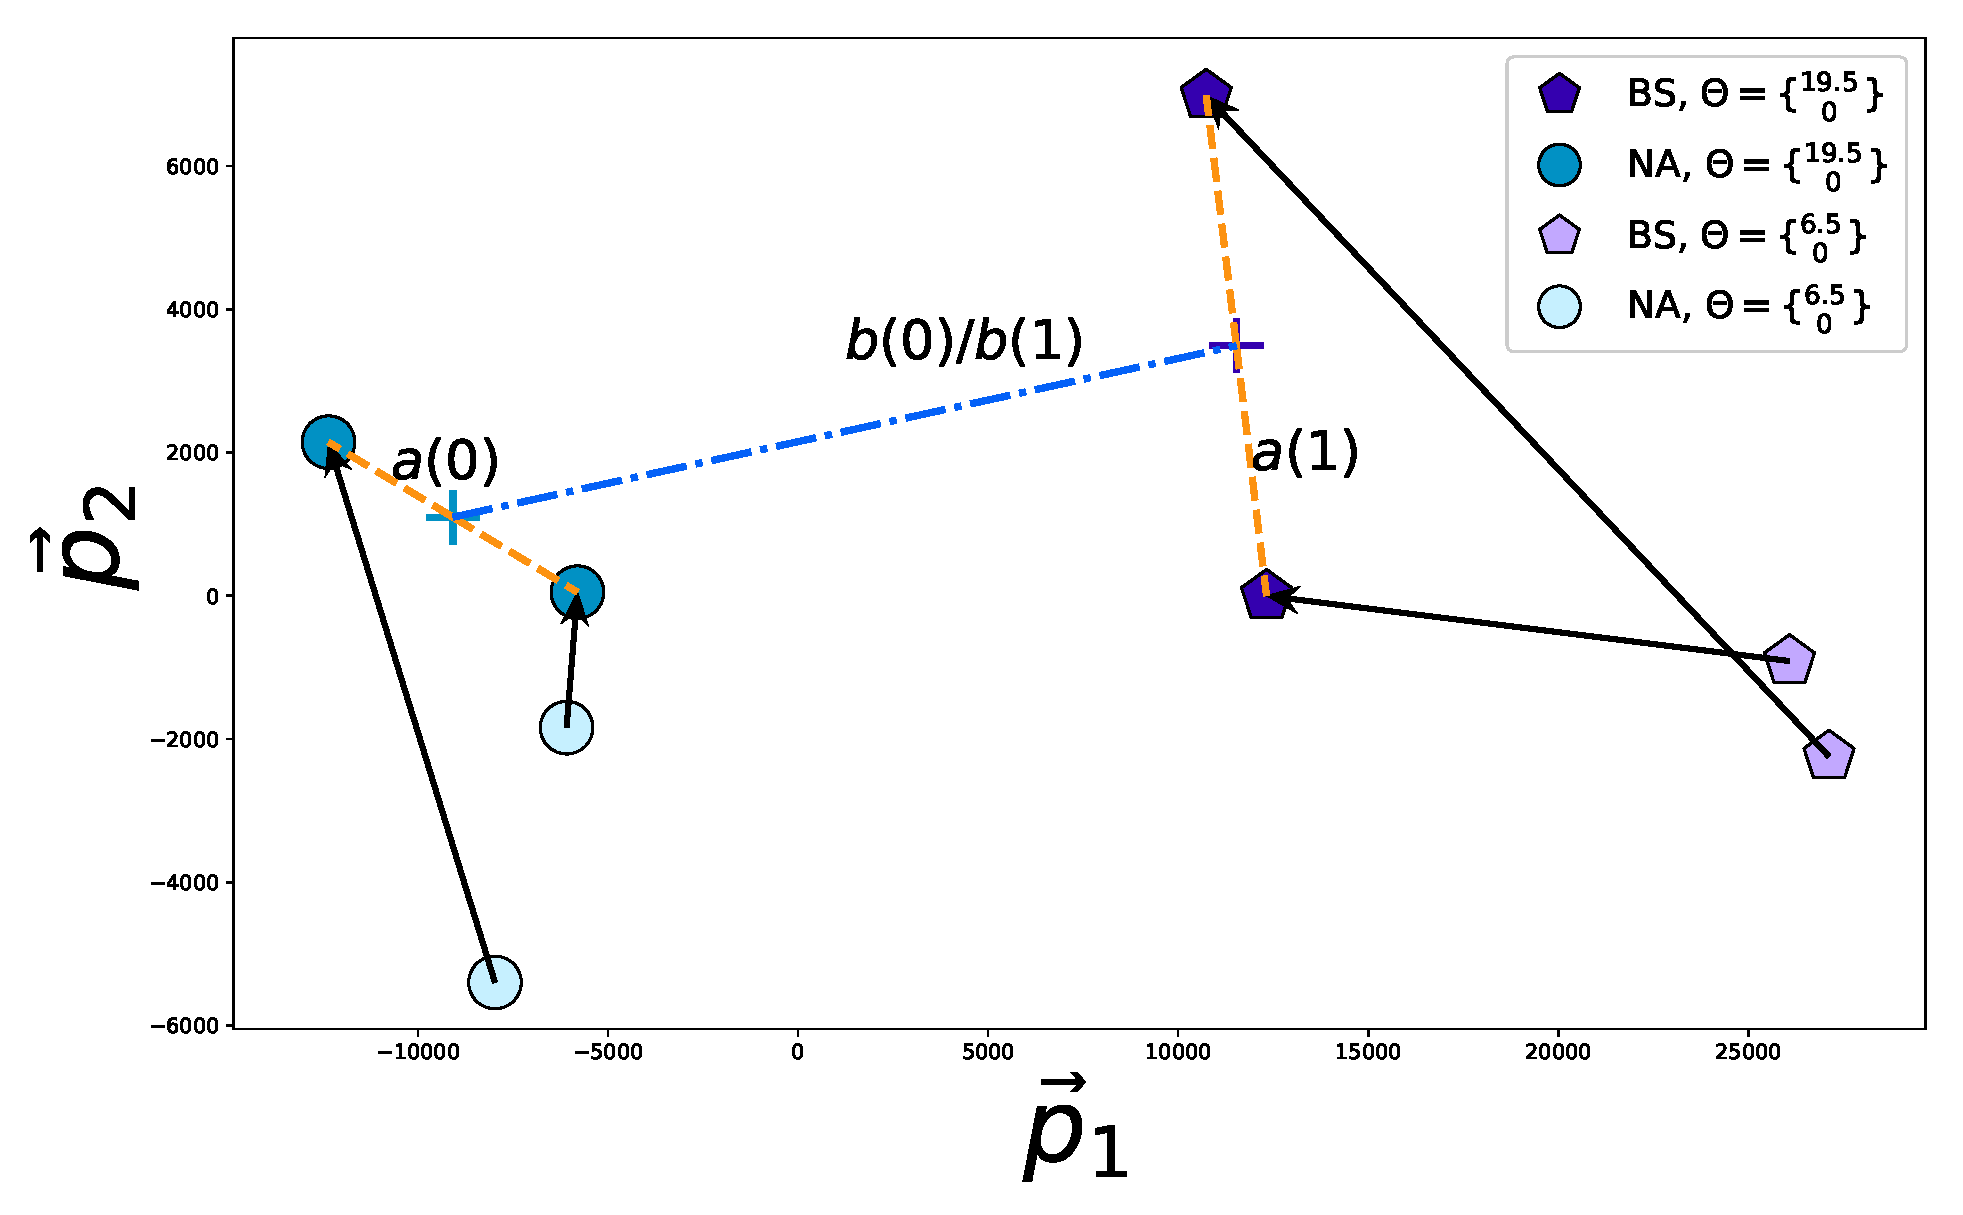
\includegraphics[width=\columnwidth]{./figs/flow.eps}
	\caption{The change in position for the 2D PCA projected \textit{NA} and \textit{BS} samples 
		when probing the phantom vertically at a depth of $6.5mm$ and $19.5mm$. The yellow and blue line 
		show the two parameters on which the silhouette score is based, i.e. intra-cluster distance and 
		nearest cluster distance respectively.}
	\label{flow}
\end{figure}
We further explore the way the probing strategy, and the properties of the probed areas in the  phantom,
affect the amount of information retained after dimensionality reduction. The explained variance achieved
prior to categorization is $I = \tau_1+\tau_2$. Fig. \ref{inf_retention_quantity:rotation} 
shows the explained variance trends when the number of probed areas used for $PCA$ projection varies. 
When the number of probed areas in maximal (16 areas, red plot in Fig. \ref{inf_retention_quantity:rotation}), 
the influence of $\Theta$ is negligible. Conversely, with less data to base the $PCA$ projection on (2 areas, 
blue plot in Fig. \ref{inf_retention_quantity:rotation}), the choice of $\Theta$ can be the sole determinant to
induce structure in the data. 
A second interesting phenomenon can be observed in Fig. \ref{inf_retention_quantity:vertical},  
when comparing the explained variance obtained after projecting $\mathbf{X}$ based on 4 vs 8 probing areas in
the phantom (yellow vs green plots). Here, the agent retains more information, even when basing the projection 
on less data, if the employed probing is vertical and at a depth of at least $17.5mm$. This result suggests that 
proper physical interaction can help information retention in the absence of enough data.


Ultimately, we observe the influence of the quality of the data samples to the information retention after 
PCA projection. Fig. \ref{inf_retention_quality:vertical} shows how in presence of very diverse inclusion types 
(left triangle plot), the effects of the vertical probing strategy $\Theta$ to $I$ is negligible. The presence of 
very diverse data, in fact, is useful for $PCA$ to find good projection axis. 
In absence of good data, or non-diverse inclusion types, instead, appropriate interaction can minimize 
information loss (peaks in Fig. \ref{inf_retention_quality:vertical} and \ref{inf_retention_quality:Rotation}).
In the figures, it is possible to see how the least diverse set of samples can yet induce 
the tactile information to retain most of the information when  the phantom is appropriately probed 
(peak in triangle plot, Fig. \ref{inf_retention_quality:vertical}).


\subsection{Information Structure and Silhouette Coefficient} \label{sec_inf_struct}


\begin{figure*}[]
	\centering
	\begin{subfigure}[b]{\columnwidth}
		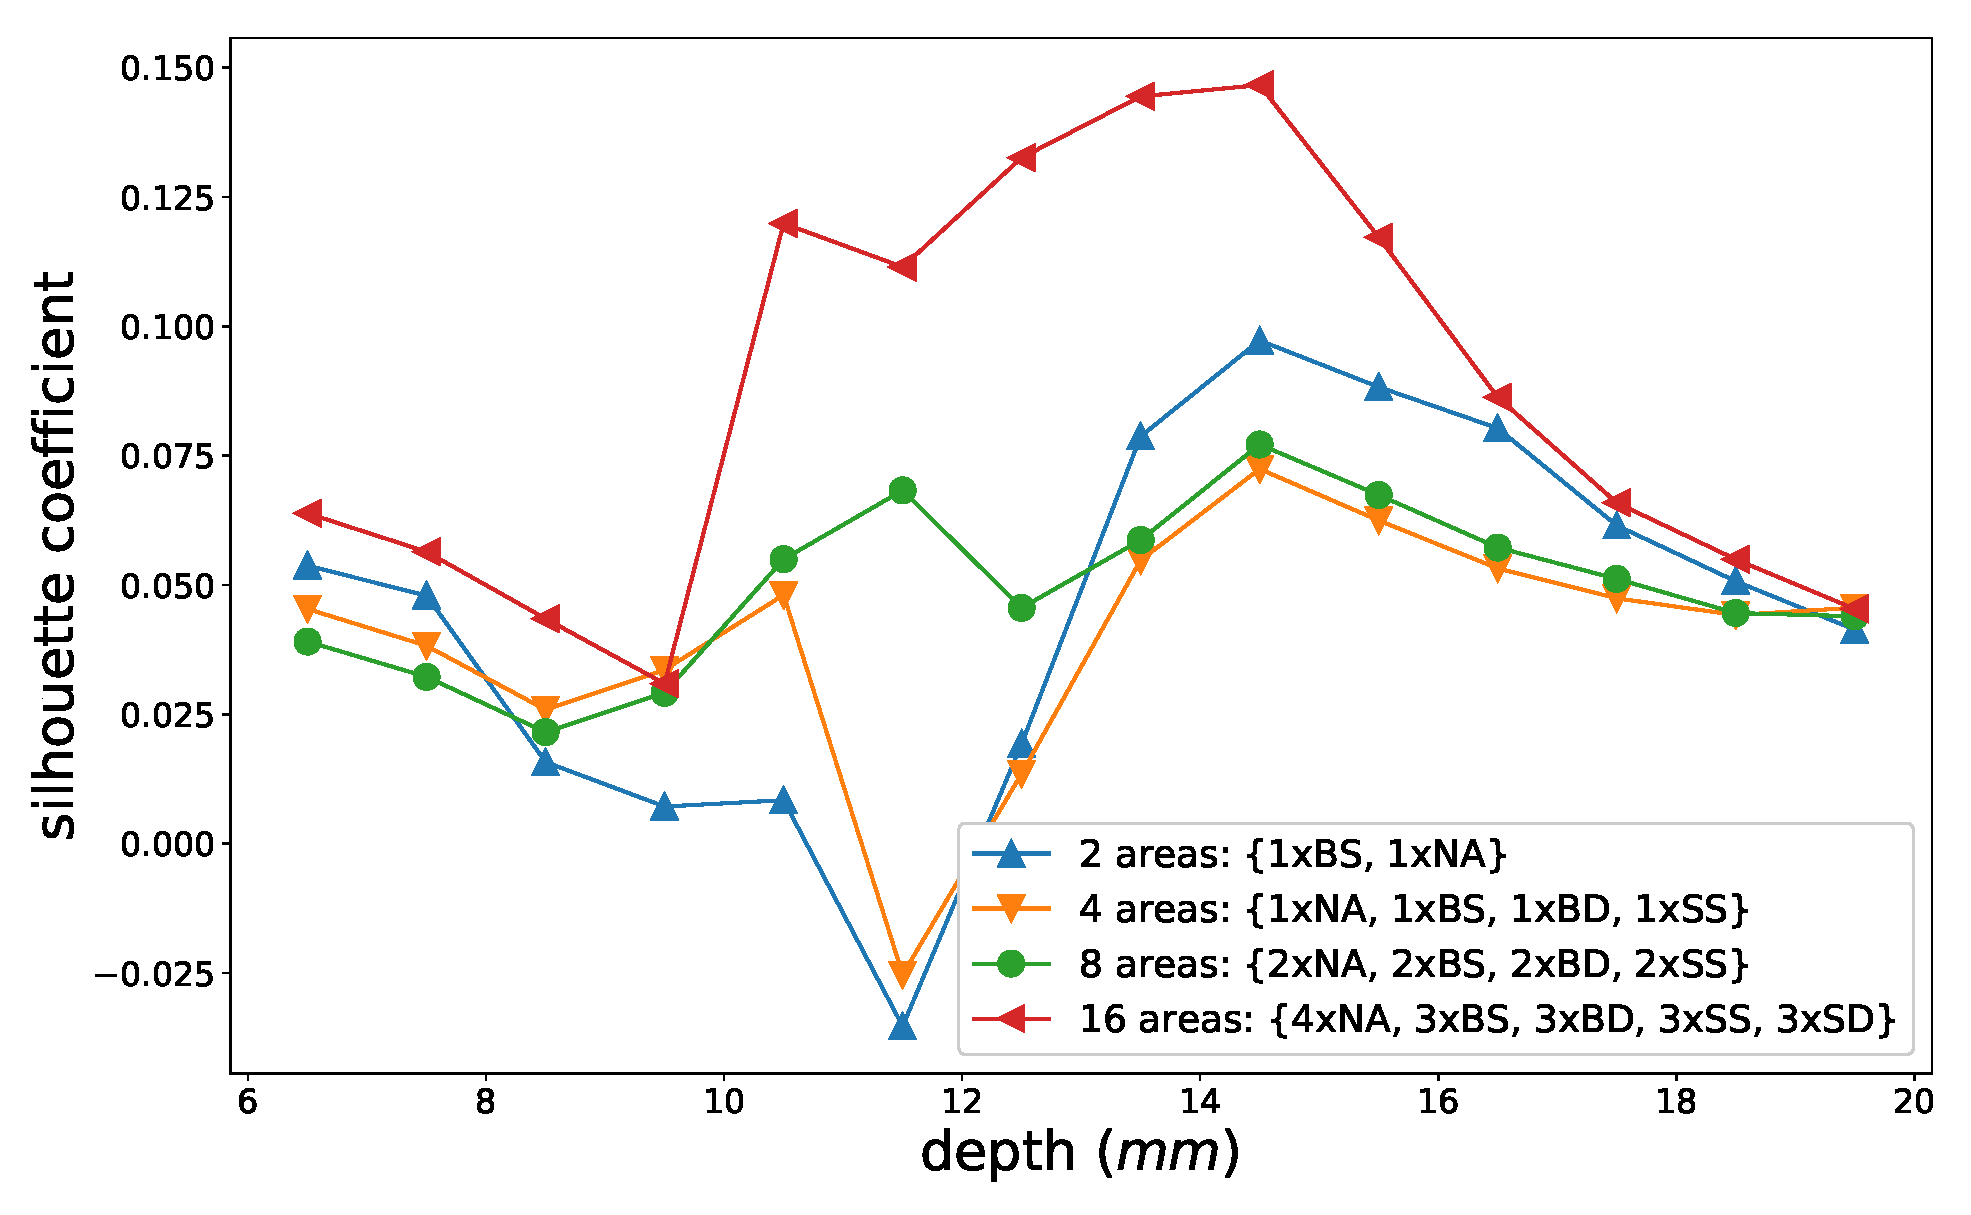
\includegraphics[width=\textwidth]{./figs/silhouette_coefficient_vertical_quantity.eps}
		\caption{$Ph\text{-}2$: Vertical Probing}
		\label{silhouette_quantity:vertical}
	\end{subfigure}
	\begin{subfigure}[b]{\columnwidth}
		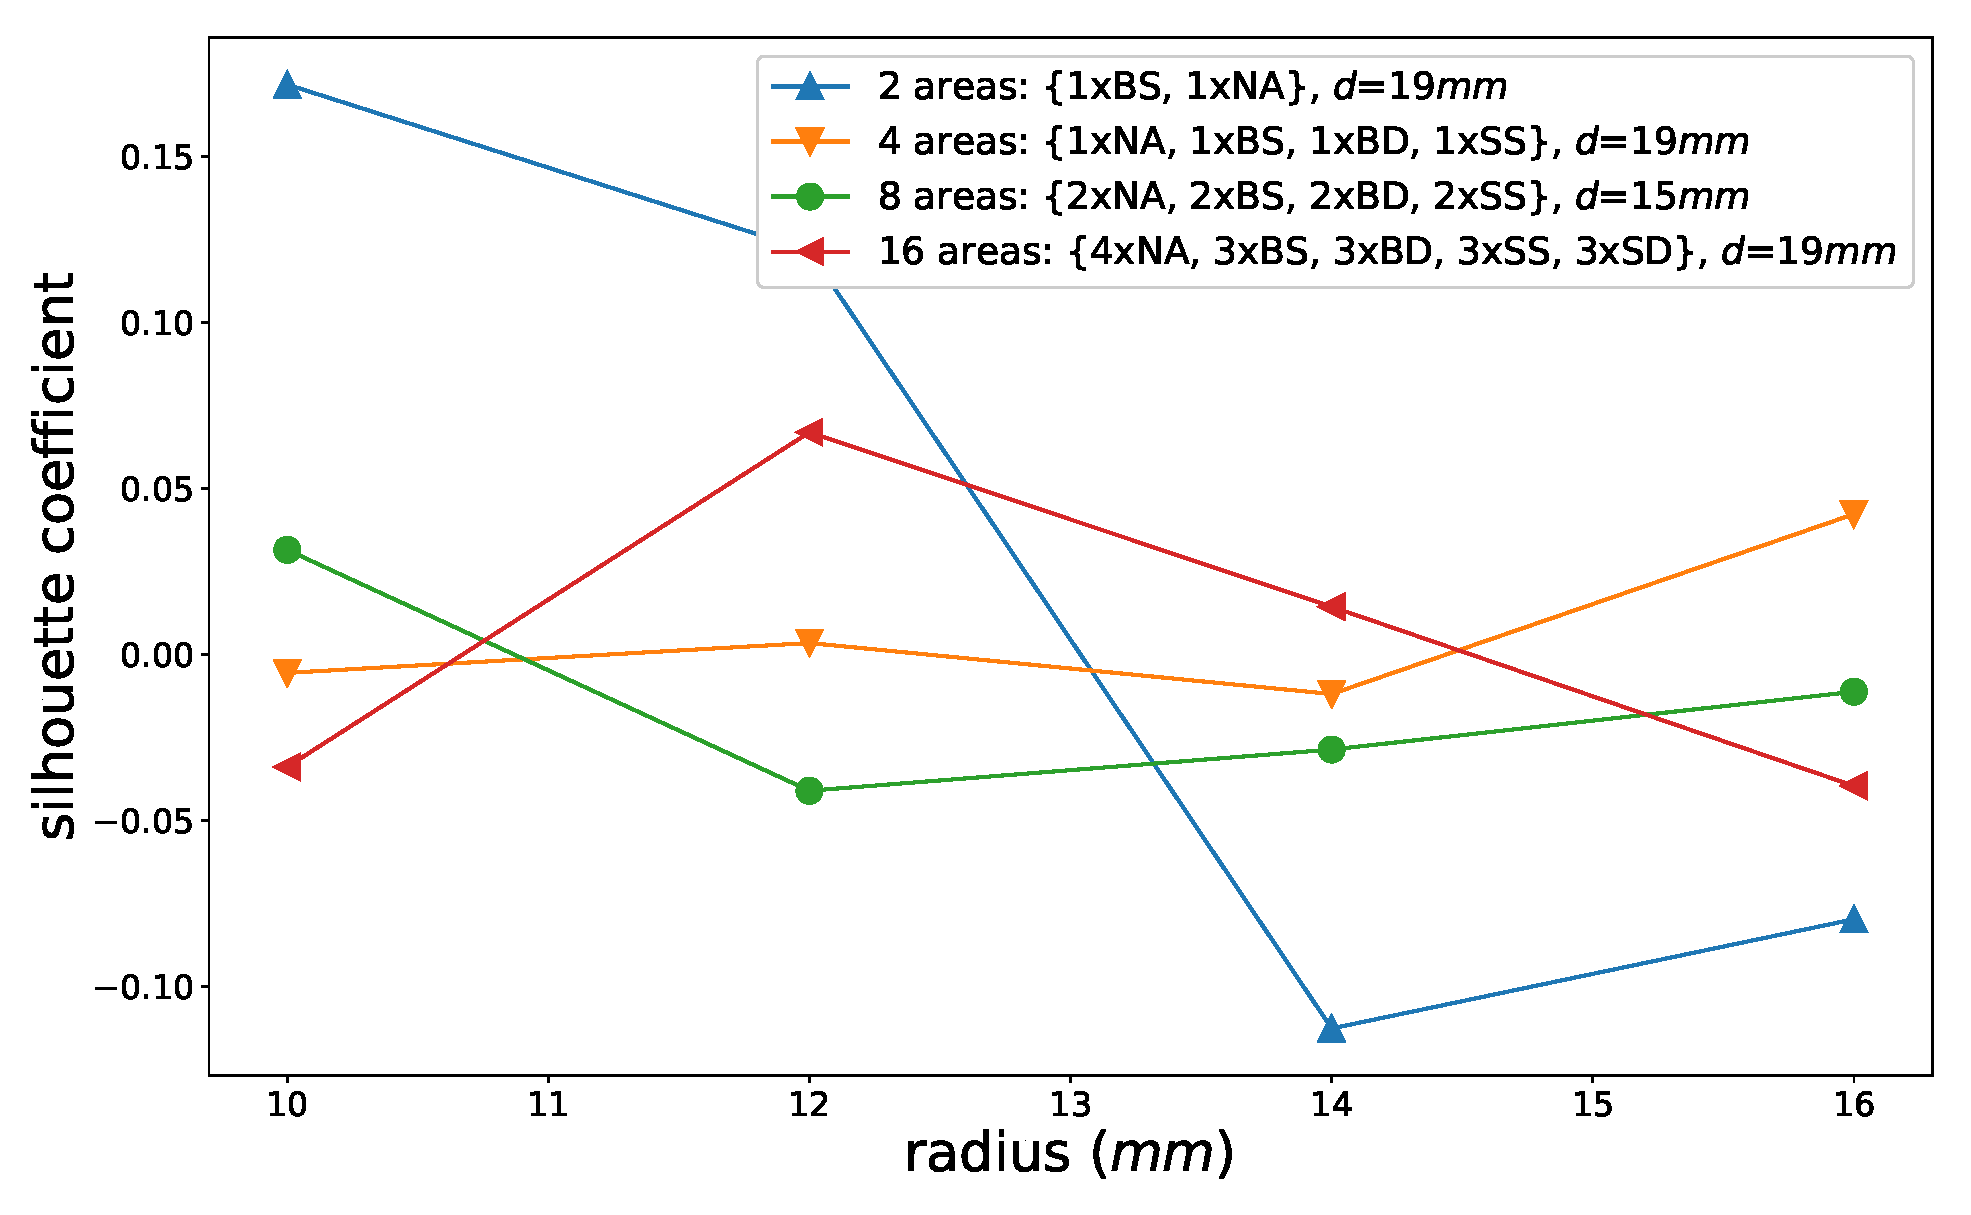
\includegraphics[width=\textwidth]{./figs/silhouette_coefficient_rotation_quantity.eps}
		\caption{$Ph\text{-}2$: Rotational Probing}
		\label{silhouette_quantity:Rotation}
	\end{subfigure}
	\caption{The change in silhouette coefficient by the 2D PCA subspace projection, 
		when probing vertically (a) and through the rotatory motion (b), changing the number of samples 
		used to find the principal components ($N$ in $\mathbf{X}$, see Section \ref{sec_dim_reduction}). }
	\label{silhouette_quantity}
\end{figure*}
\begin{figure*}[]
	\centering
	\begin{subfigure}[b]{\columnwidth}
		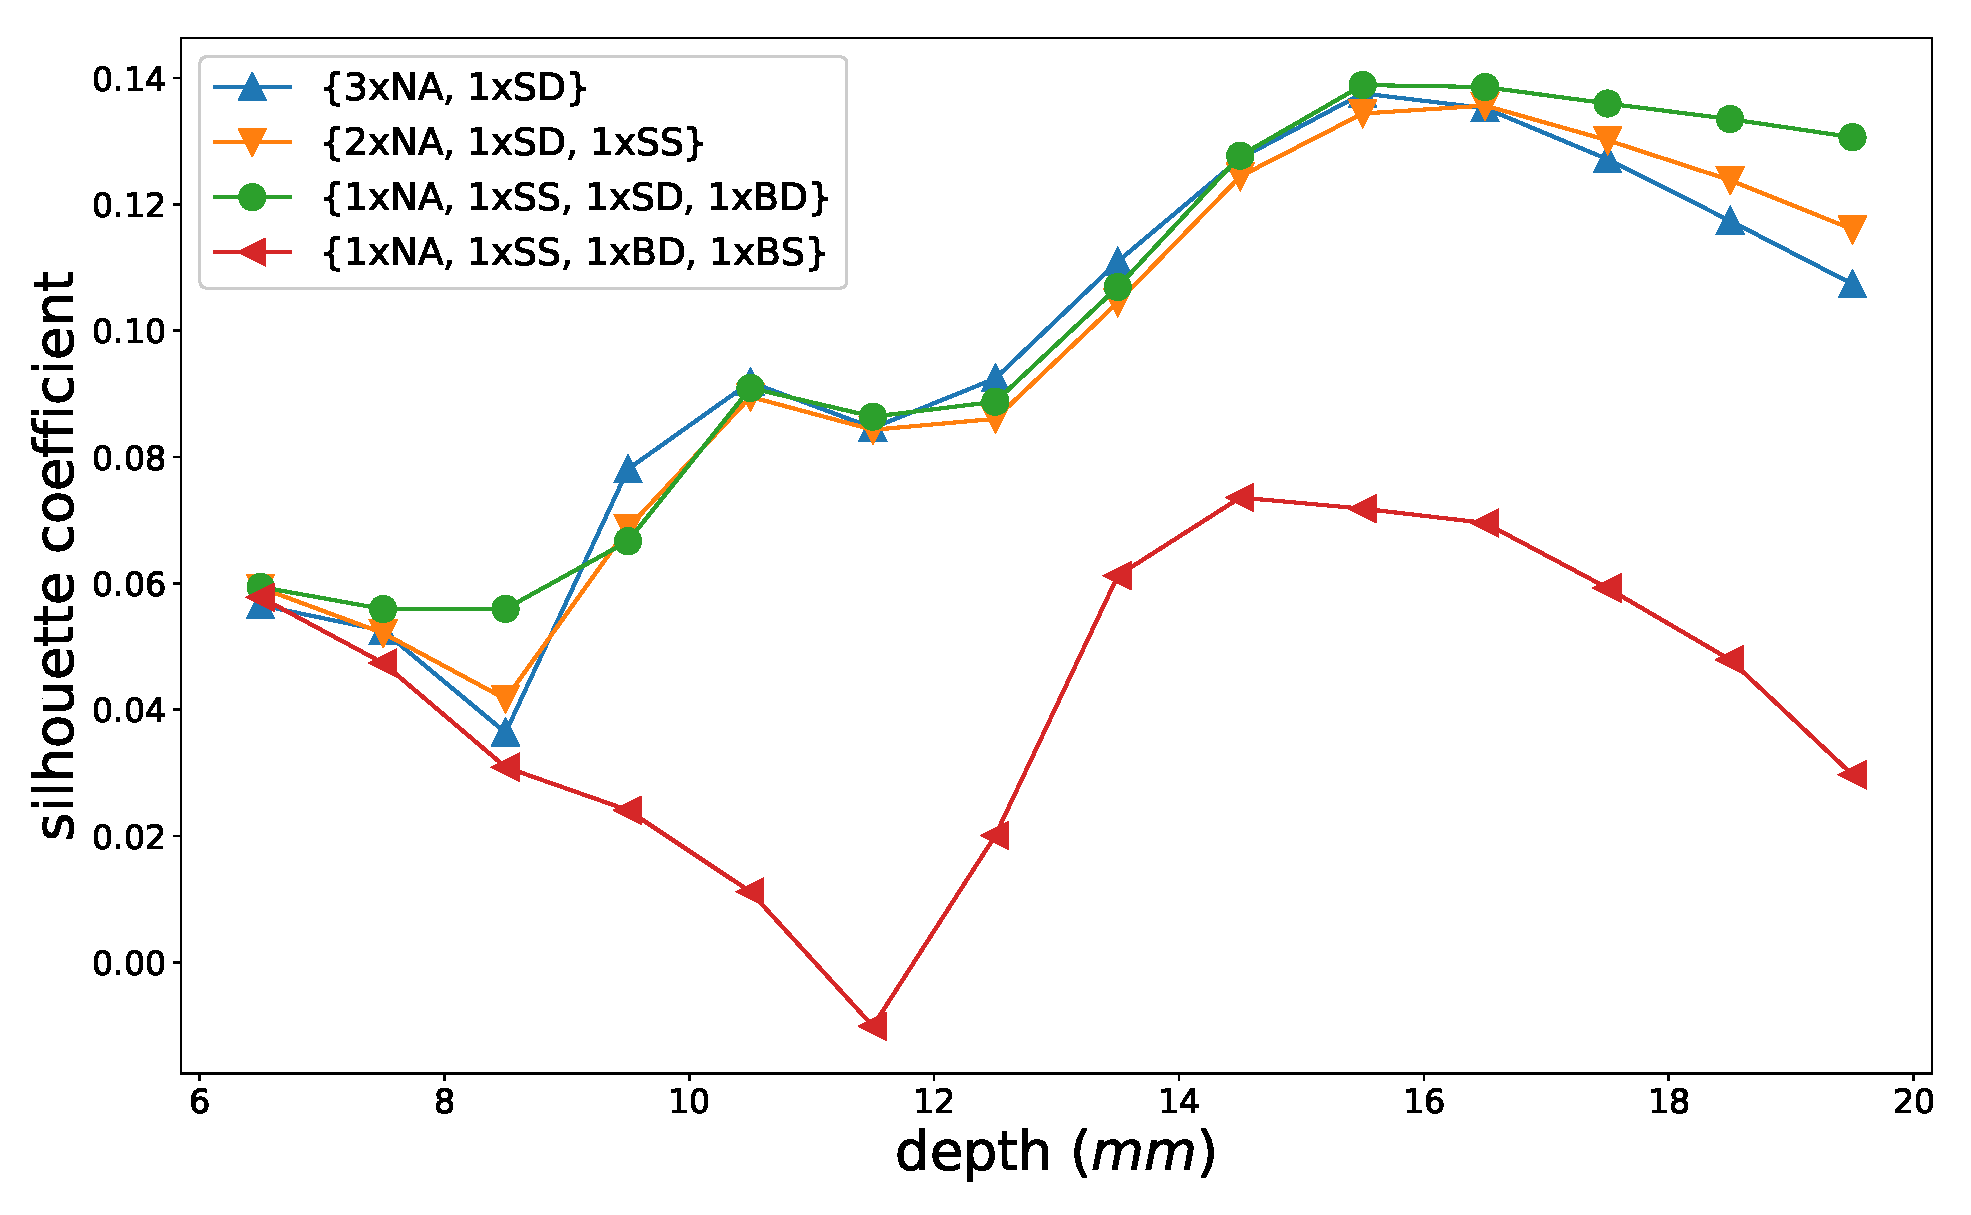
\includegraphics[width=\columnwidth]{./figs/silhouette_coefficient_vertical_quality.eps}
		\caption{$Ph\text{-}2$: Vertical Probing}
		\label{silhouette_quality:vertical}
	\end{subfigure}
	\begin{subfigure}[b]{\columnwidth}
		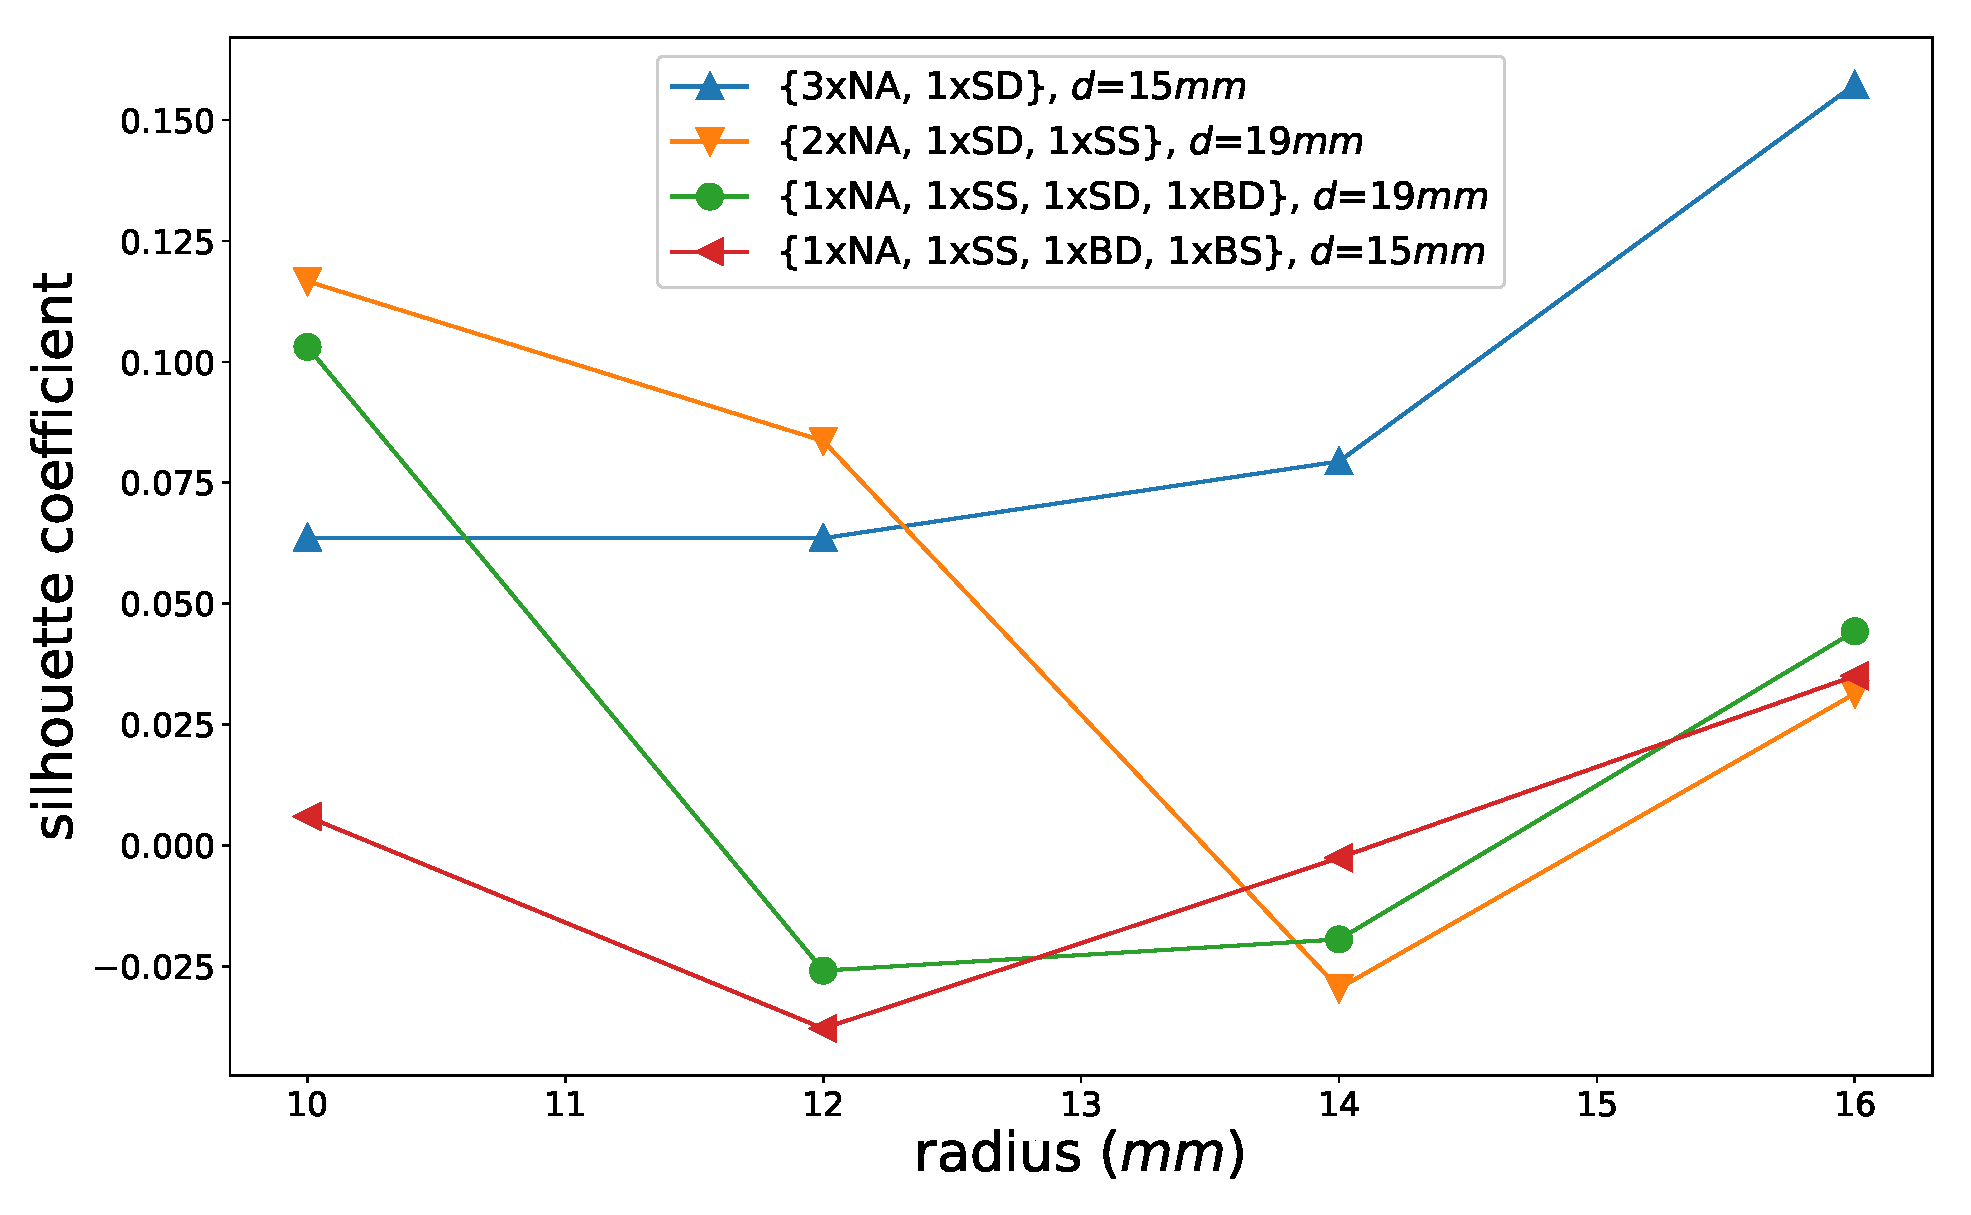
\includegraphics[width=\columnwidth]{./figs/silhouette_coefficient_rotation_quality.eps}
		\caption{$Ph\text{-}2$: Rotational Probing}
		\label{silhouette_quality:Rotation}
	\end{subfigure}
	\caption{The change in silhouette coefficient by the 2D PCA subspace projection, 
		when probing vertically (a) and through the rotatory motion (b), changing the quality of the 
		samples used to find the principal components, while maintaining their number constant. }
	\label{silhouette_quality}
\end{figure*}
\begin{figure}[]
	\centering
	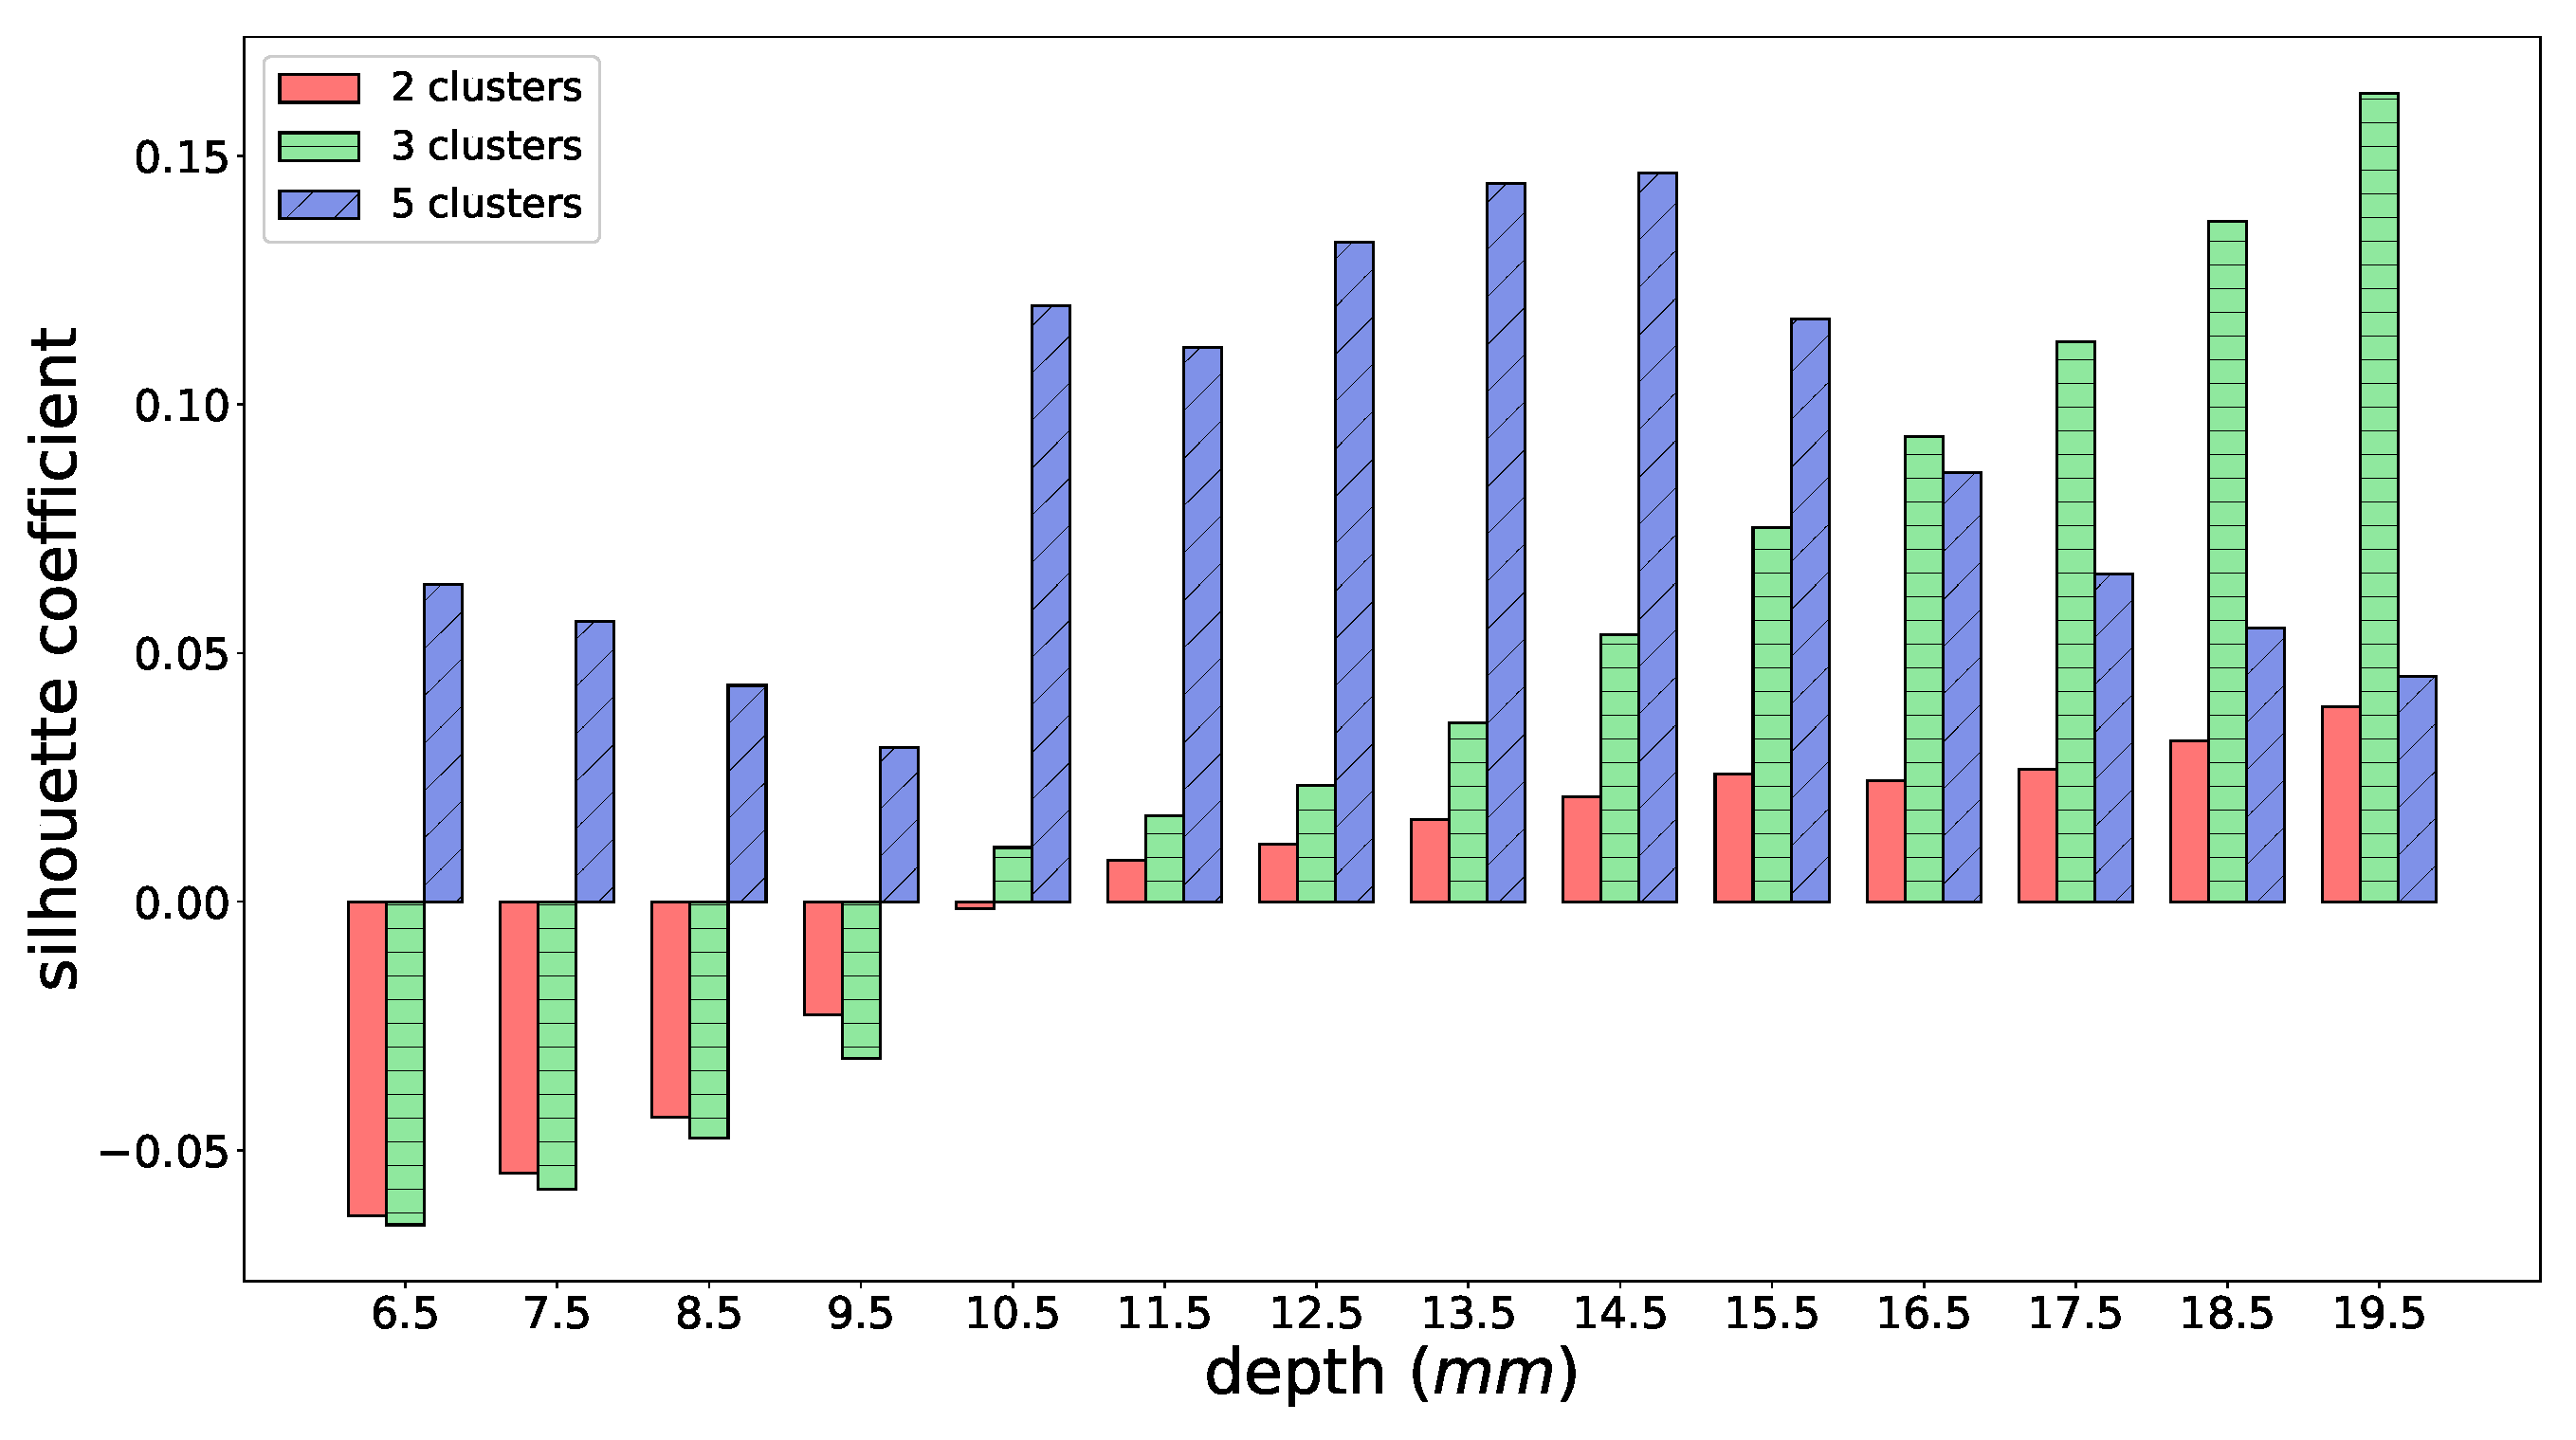
\includegraphics[width=\columnwidth]{./figs/bar_clst_num_change.eps}
	\caption{The silhouette score of PCA projected tactile sensor information for every probing area in the 
		soft phantom, when performing the probing action at different depths, and over varying number of 
		clusters.}
	\label{clst_number}
\end{figure}

Similarly to the previous sections we wish to observe the effects of changing the $\Theta$ parameters
to the structure of the information after $PCA$ projection. The silhouette coefficient, as explained in Section \ref{sec_sil_coeff}, depends on the mutual mean intra-cluster distance, and mean nearest-cluster distance for each pair of clusters (Fig. \ref{flow}).

Fig. \ref{silhouette_quantity} and Fig. \ref{silhouette_quality} both show how the change in $\Theta$ 
influences the silhouette score. This influence, however, is primarily dependent 
on $N$ and the diversity of the inclusions probed, as suggested by the change in 
trends of the plots in each of the figures. Fig. \ref{silhouette_quantity:vertical} shows 
that little structure emerges when probing $Ph\text{-}2$ vertically too superficially or too deeply. 
In both cases, in fact, the sensor response is uniformly too moderate or too steep to have any variation 
from an area of the phantom to another, thus inducing no variation in the information. Fig. 
\ref{silhouette_quantity:Rotation}, instead, shows how, when in absence of enough data samples (2 areas, blue plot), 
a correct choice of $\Theta$ can be the sole determinant for good or bad structure in the information. 
In Fig. \ref{silhouette_quality:vertical} and Fig. \ref{silhouette_quality:Rotation}, interestingly, it is shown 
how even without much diversity in the inclusion types, good structure can emerge when the phantom is probed appropriately
($\Theta = \small{\begin{Bmatrix}16.5\\ 0\end{Bmatrix}}$ or $\Theta = \small{\begin{Bmatrix}14.5\\ 16\end{Bmatrix}}$ ).


At last, we investigate the influence of the number of clusters $K$ to the structure of the information $s$. 
The number of clusters sets the level of abstraction that the robot may wish to have to make use of the tactile 
information, and directly affect the interpretation of the emerging clusters. We choose three 
varying number of clusters: $K=2$, presence vs. absence of an hard inclusion; $K=3$, absence vs. small vs. large 
inclusion; $K=5$, all inclusion types. Fig. \ref{clst_number} shows the trends when probing the soft phantom 
vertically at varying depths and changing $K$ in the $KMC$ algorithm. The emerging 
clusters present different structural properties. The different trends in the figure suggest how $K$ directly 
affect the way the probing strategy influences the structure of the data. Interestingly, 
probing at a deeper depth increasingly helps to sense inclusions, or detect their size. 
To dissociate between all different inclusion types, instead, an optimal probing depth is found for $d=14.5mm$, 
after which the increasingly high sensor response converges, and renders the clusters less separable, thus 
decreasing the values of $s$.


\subsection{Motion influence on Cognitive Maps}

Predicting the effects of $\Theta$ to the low-level encoding of the information in $\mathbf{W}$ is a 
highly complex process. Understanding such effects, however, would allow an agent to appropriately choose
a $\Theta$ when solving the probing task.

To understand this relationship we make a plot of the cognitive maps for each set of motion parameters in $\Theta$ 
and observe how the encoding of each probed area changes according to the probing strategy used. Here, 
to have a better understanding of the motion effects, we perform the experiment on the least cluttered 
phantom, i.e. $Ph\text{-}1$ (Fig. \ref{ph2}), which would suffer less from disturbances due to the vicinity 
of adjacent inclusions. 
Figure \ref{ResVert:dn0} and \ref{ResVert:dn9} show the plots corresponding to probing the phantom 
vertically at the minimal and maximal experimental depth. By increasing the depth of probing, two very interesting 
effects take place: one, nearest cluster distance $b(i)$ between almost all types of inclusions increases, 
allowing for better dissociation of diverse tactile information; two, the intra cluster distance $a(i)$ 
between any two probing areas with the same type of hard inclusion decreases, allowing for each 
possible phantom inclusion type to be better represented. 

Extending the analysis to the rotational probing strategy we can similarly observe the effects of 
changing the parameters in $\Theta$ from their minimal to their maximal experimental values. 
Interestingly, when employing the rotational strategy, the generated tactile information presents a 
structured layout, by which it is already possible to dissociate one stimulus type from another. In this 
scenario, then, the effect of the rotational parameter $r$ to the structure of the data $s$ appears to 
only mildly act upon the nearest-cluster distance parameter (Fig. \ref{ResRot:100-100} to 
Fig. \ref{ResRot:100-160}). The effect of increasing $d$, instead, confirms the hypothesis 
by which the probing depth influence acts upon the intra cluster distance of each stimulus type.  

The effect of the depth parameter can be attributed to the strength in response of the sensorised probe. 
The tactile sensor, in fact, detects pressure levels on its surface. When probing the phantom at the minimum 
depth, the pressure registered by the sensor is mostly due to the elastic response of the Ecoflex 00-10 soft 
phantom, almost independently from the presence or absence of inclusions in the probed area. As the depth 
increases, the elastic response is influenced by the non-elasticity of the hard inclusion, should there be 
one in the probed area. We hypothesize this influence can be captured by the sensor response in three ways: 
first, the response should be higher when inclusions are present in the probed area; second, the sensor's increase 
in detected pressure should arise at slightly different sample intervals depending on where the inclusion is placed 
in the phantom (deep vs shallow inclusion); third, the area of the response should vary depending on the 
size and depth of the inclusion. 

In this framework, an acceptable probing depth is one which neither saturates the sensor response in each area, 
nor fails to detect changes in pressure when the probed area contains non-elastic inclusion. The task of 
dissociating amongst all different types of inclusions is optimized (i.e. maximal silhouette score) for
$\Theta = \tiny{\begin{Bmatrix}12.5\\ 0\end{Bmatrix}}$ in $Ph\text{-}1$ and 
$\Theta = \tiny{\begin{Bmatrix}14.5\\ 0\end{Bmatrix}}$ in $Ph\text{-}2$.

\subsection{Categorization and Similarity Abstractions}
In robotics palpation, proper physical interaction can help in the dissociation 
of tactile information, such that the emerging clusters can be meaningful 
with respect to solving a task (e.g. finding hard inclusions in a soft phantom). 
Besides dissociating amongst different object types, however, another fundamental, yet usually neglected, 
fragment of information is related to the similarity associations between clusters. The distances 
between found clusters in the 2D re-encoded tactile information subspace, in fact, grants the agent 
the possibility to associate types of objects, and order or rank them based on such association.

In the context of probing a soft phantom to find hard inclusions, for example, the agent might need to 
prioritize possible findings based on the depth of the inclusion, e.g. $[$\textit{NA}, \textit{SD/BD}, 
\textit{SS/BS}$]$, we'll refer to this as rank-1. In a different scenario where the size of the hard 
inclusion should take priority over its depth, the ranking might, for example, change to 
$[$\textit{NA}, \textit{SD/SS}, \textit{BD/BS}$]$, or rank-2. In this scenario, the influence of 
the physical interactions with the soft phantom may induce the agent to see some inclusion 
types as more similar to others, depending on which property is deemed more important.

\begin{figure*}[]
	\begin{subfigure}[b]{\textwidth}
		\begin{subfigure}[b]{.48\textwidth}
			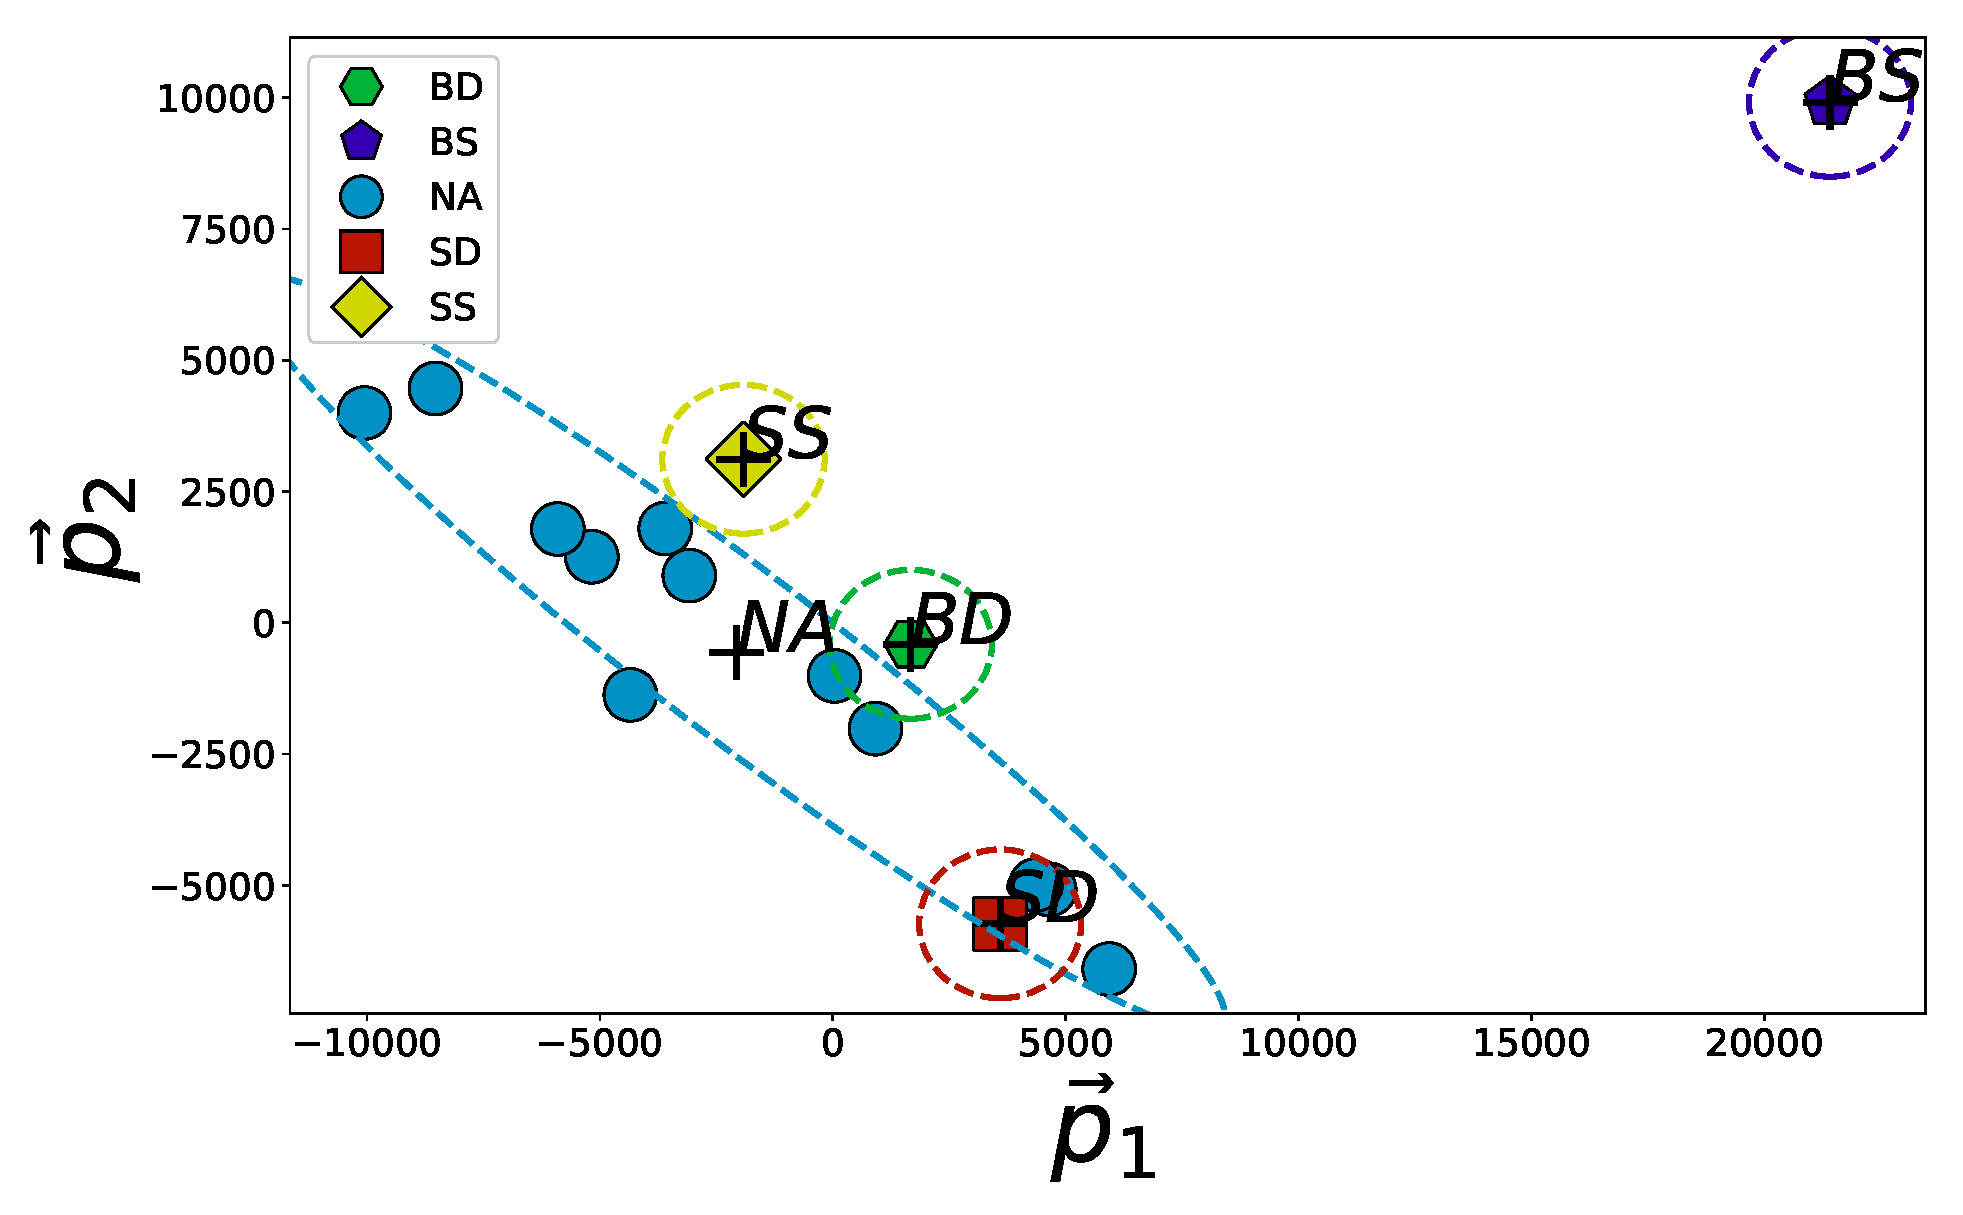
\includegraphics[width=\textwidth]{./figs/phantom1properties_clsplt_Vertical-d6_5.eps}
			\caption{$\Theta = \small{\begin{Bmatrix}6.5\\ 0\end{Bmatrix}}$}
			\label{ResVert:dn0}
		\end{subfigure} 
		\hspace{0.01\textwidth}
		\begin{subfigure}[b]{0.48\textwidth}
			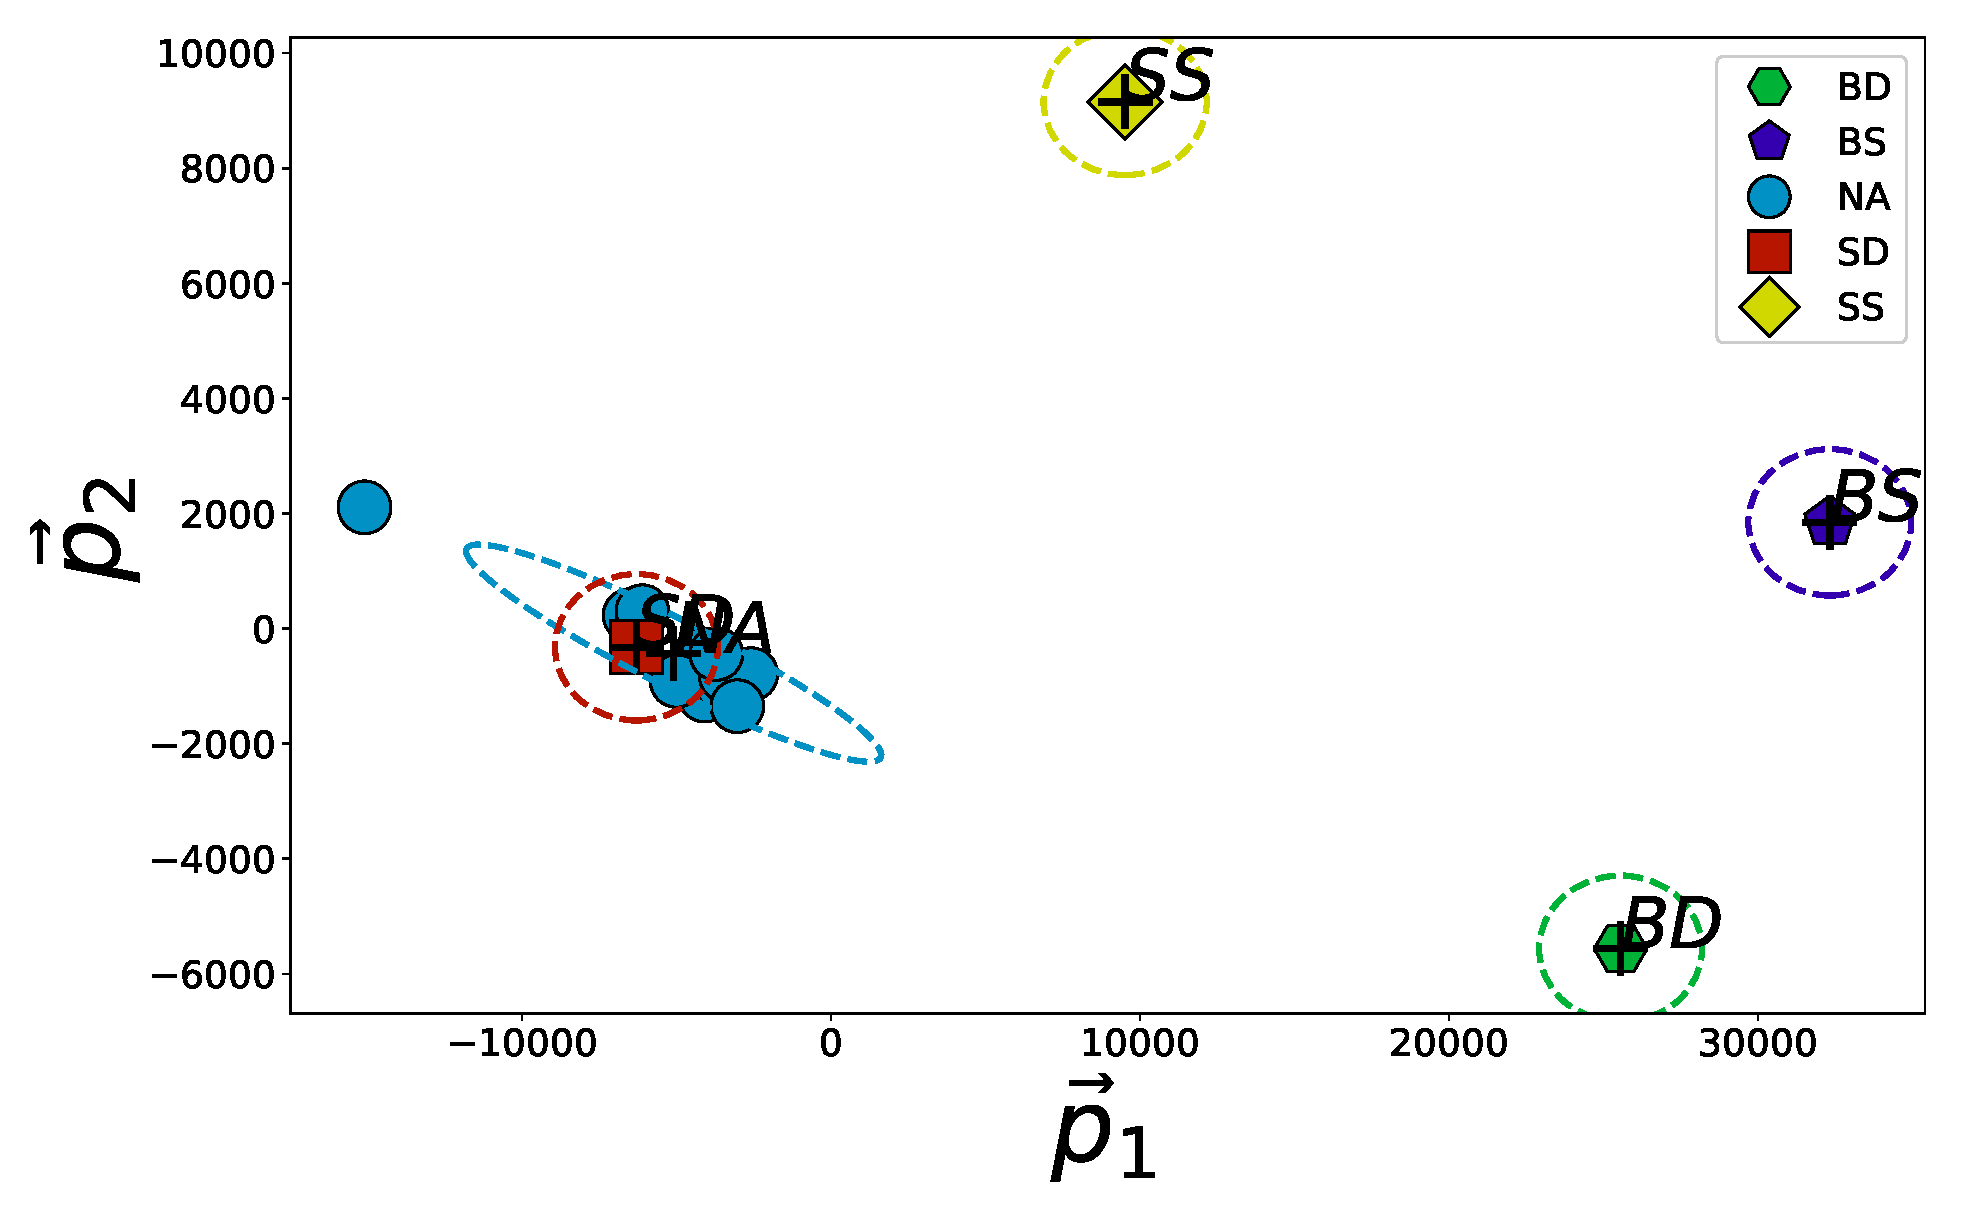
\includegraphics[width=\textwidth]{./figs/phantom1properties_clsplt_Vertical-d19_5.eps}
			\caption{$\Theta = \small{\begin{Bmatrix}19.5\\ 0\end{Bmatrix}}$}
			\label{ResVert:dn9}
		\end{subfigure}
	\end{subfigure}
	\caption{The 2-dimensional projection of the tactile information generated from probing $Ph\text{-}2$ 
		at varying depths. The ellipses correspond to the distributions of the clusters based on their true 
		inclusion types, at a distance of 2 standard deviations from their respective cluster center.}
	\label{ResVert}
\end{figure*}

\begin{figure*}[]
	\centering
	\begin{subfigure}[b]{\textwidth}
		\begin{subfigure}[b]{.48\textwidth}
			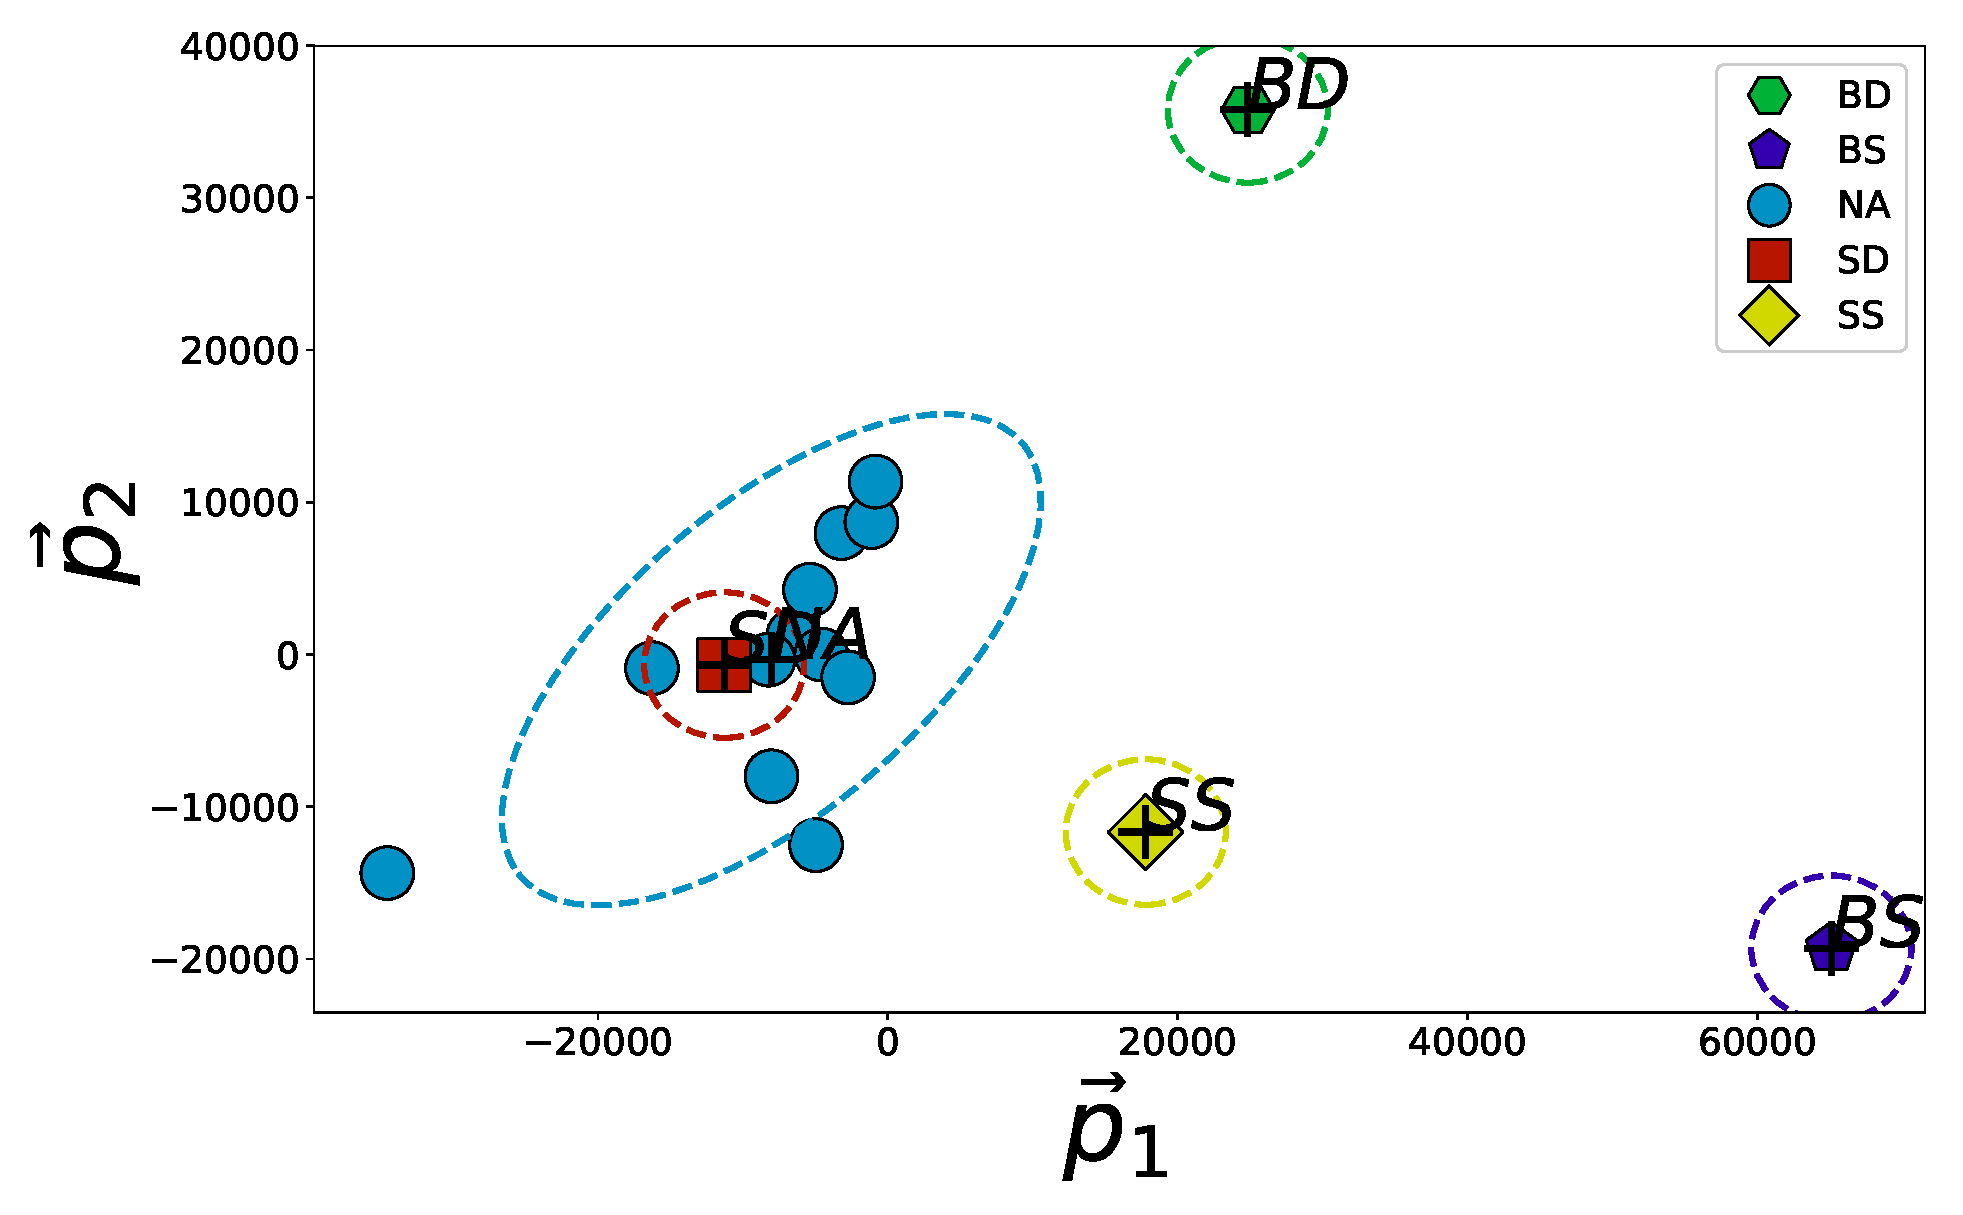
\includegraphics[width=\textwidth]{./figs/phantom1properties_clsplt_Rotate-d100-r100.eps}
			\caption{$\Theta = \small{\begin{Bmatrix}10\\ 10\end{Bmatrix}}$}
			\label{ResRot:100-100}
		\end{subfigure} 
		\hspace{0.01\textwidth}
		\begin{subfigure}[b]{0.48\textwidth}
			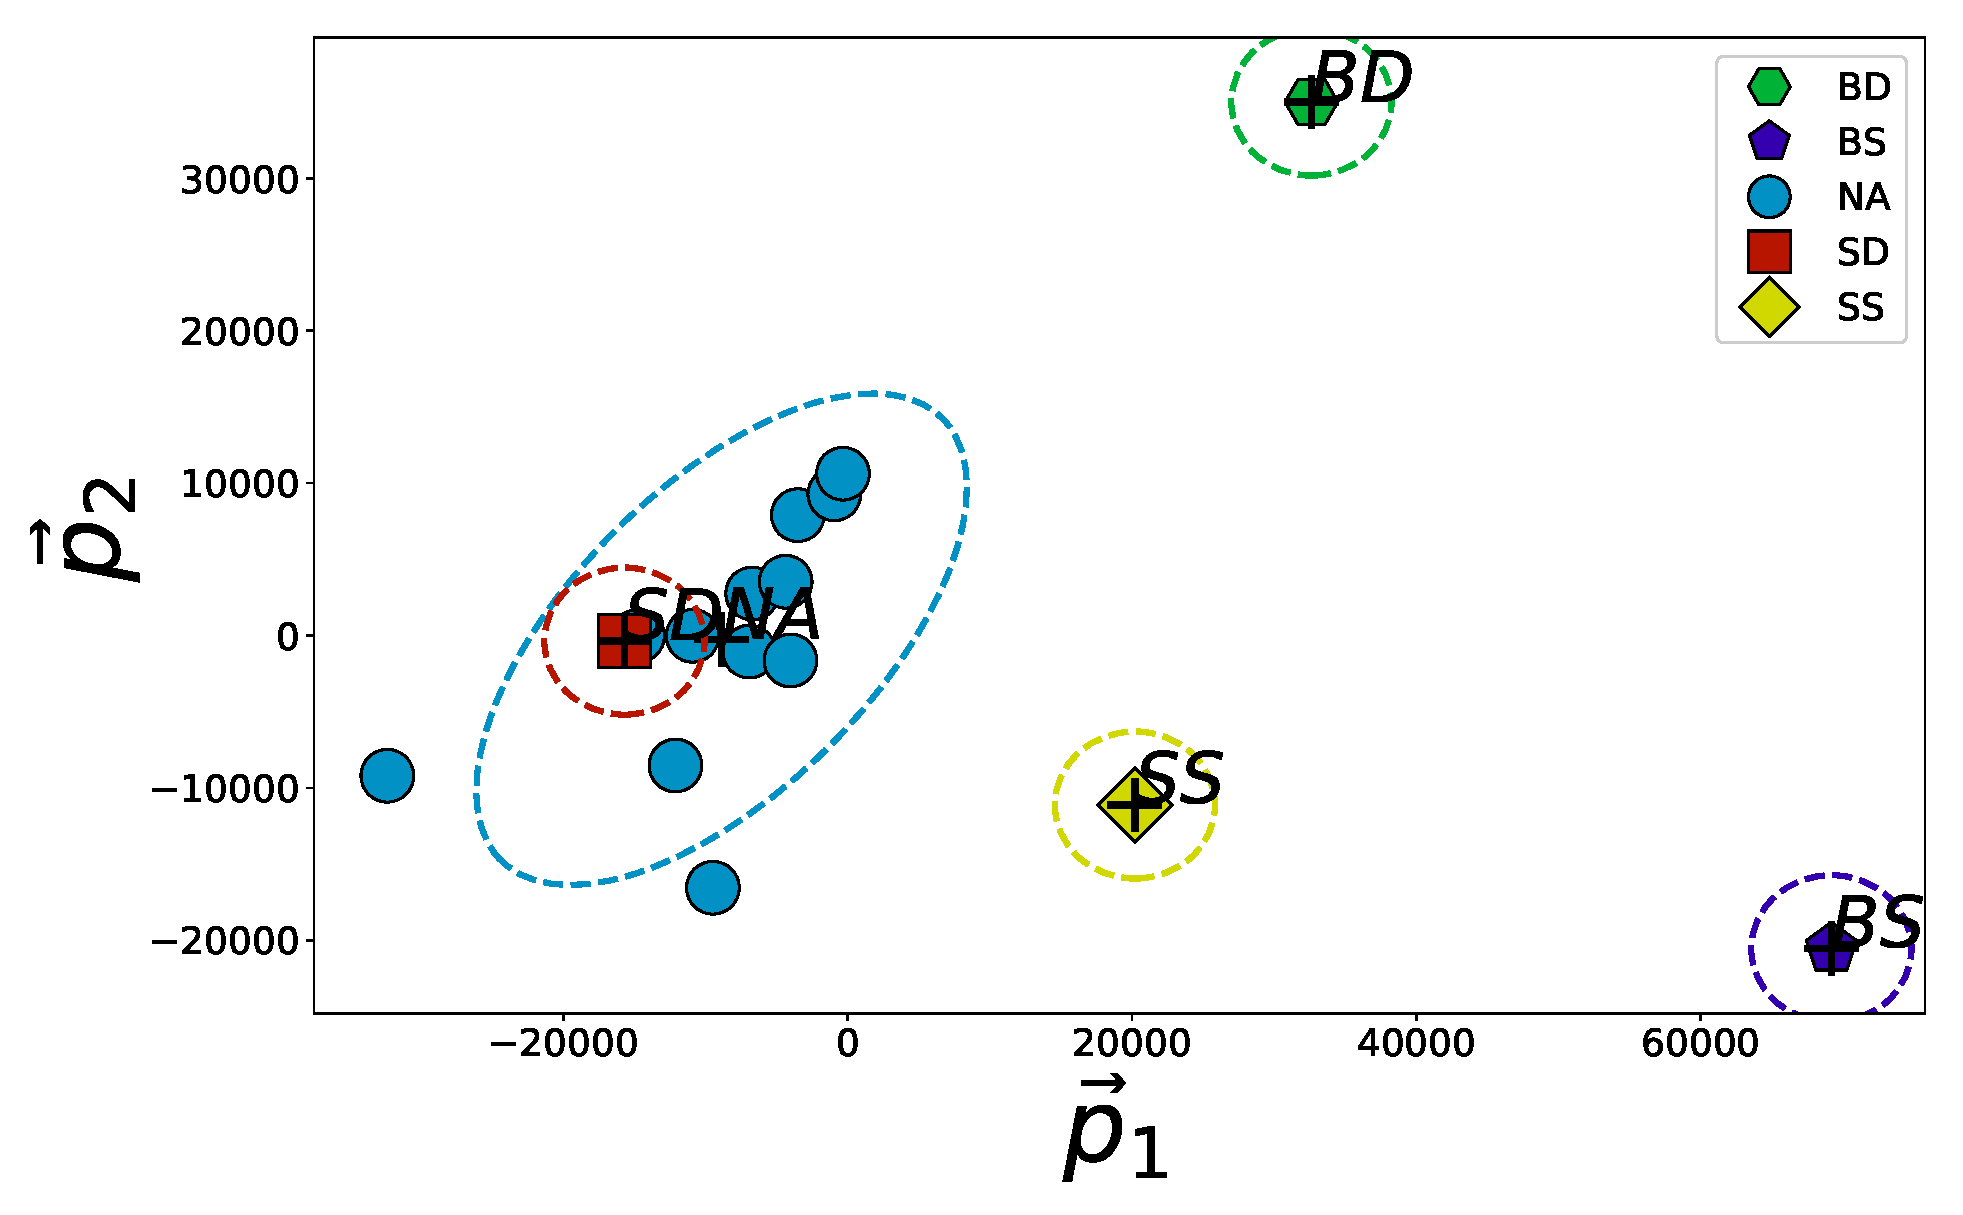
\includegraphics[width=\textwidth]{./figs/phantom1properties_clsplt_Rotate-d100-r160.eps}
			\caption{$\Theta = \small{\begin{Bmatrix}10\\ 16\end{Bmatrix}}$}
			\label{ResRot:100-160}
		\end{subfigure}
		\vspace{4pt}
	\end{subfigure}
	\begin{subfigure}[b]{\textwidth}
		\begin{subfigure}[b]{0.48\textwidth}
			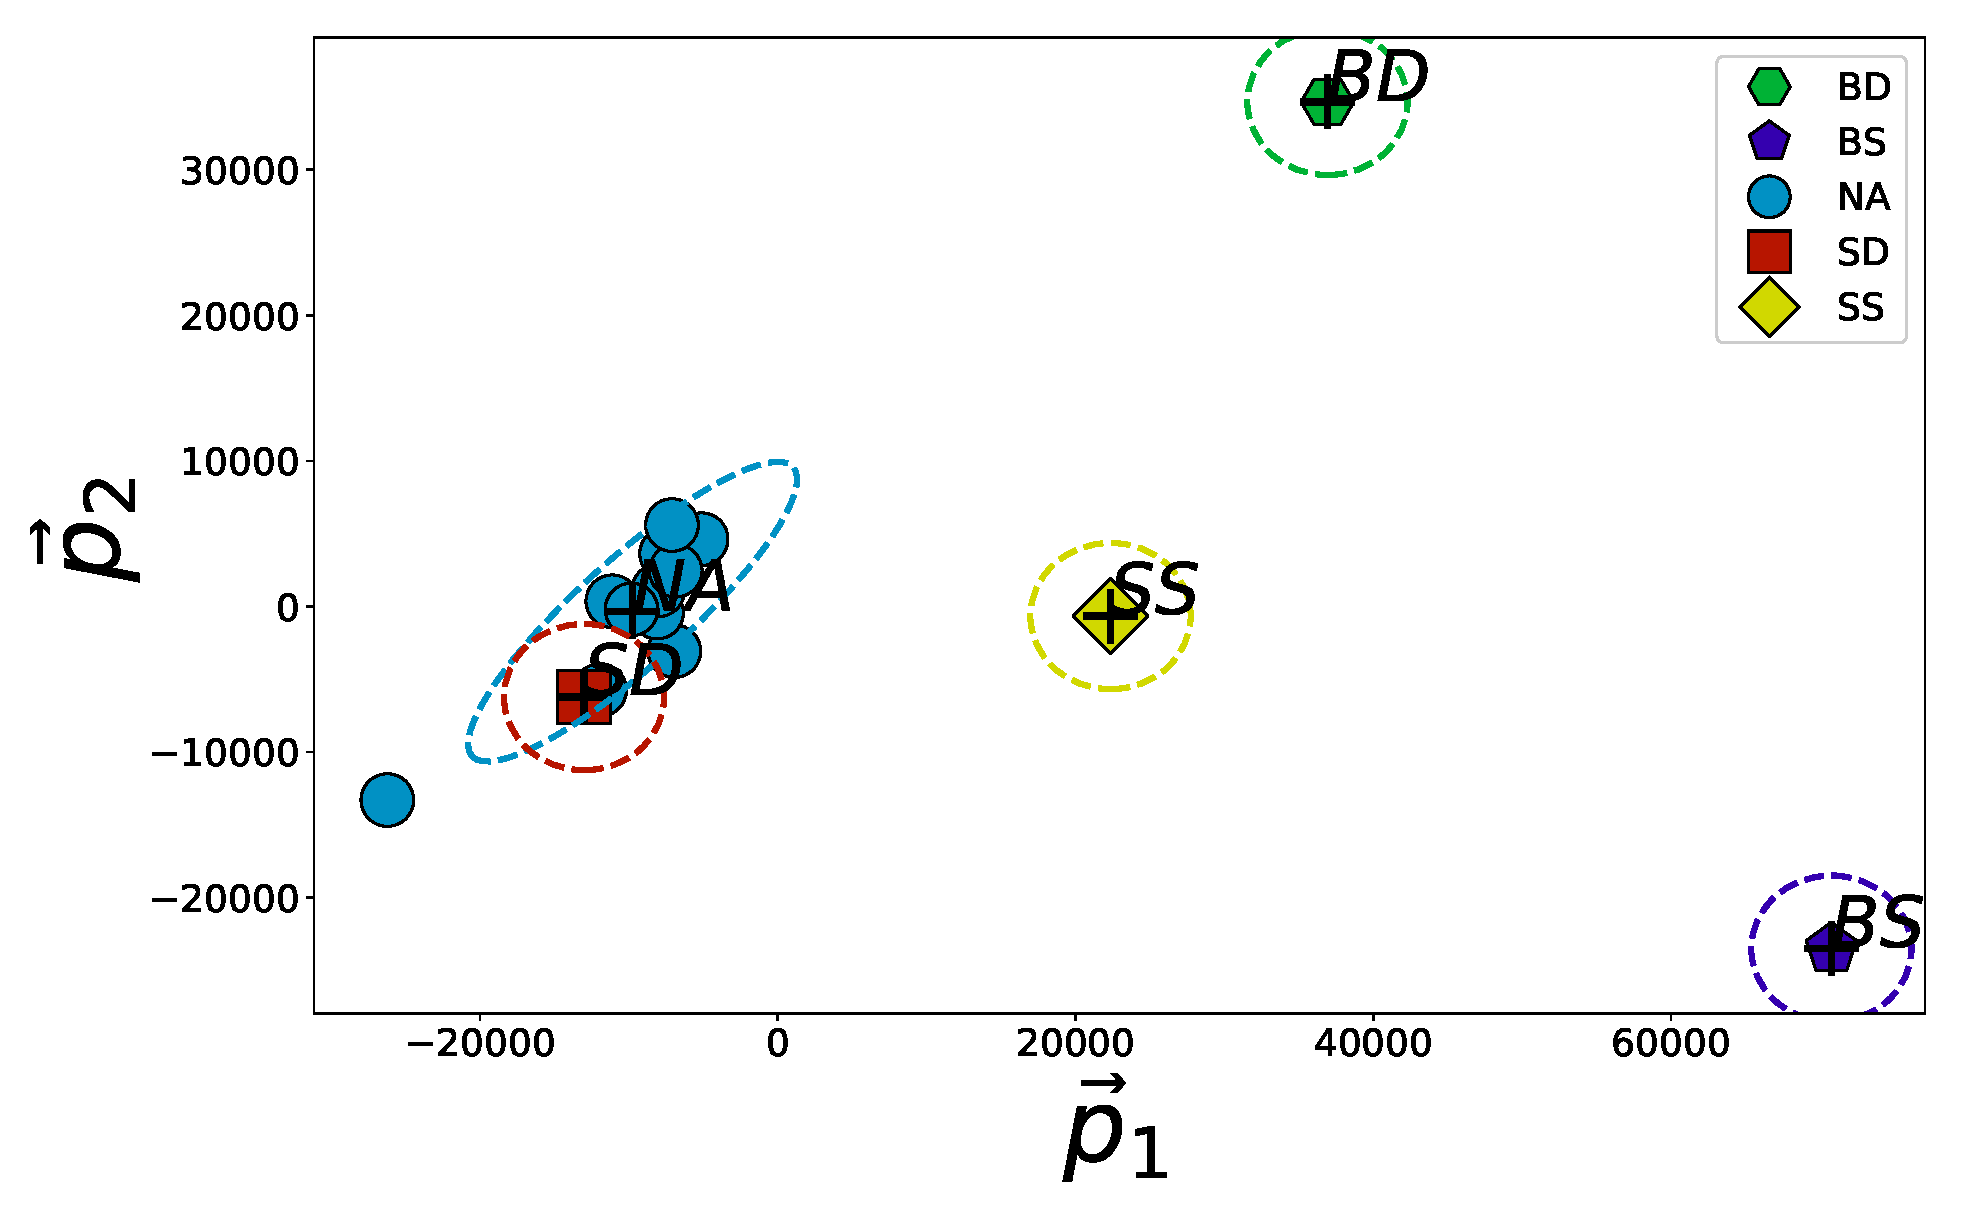
\includegraphics[width=\textwidth]{./figs/phantom1properties_clsplt_Rotate-d160-r100.eps}
			\caption{$\Theta = \small{\begin{Bmatrix}16\\ 10\end{Bmatrix}}$}
			\label{ResRot:160-100}
		\end{subfigure}
		\hspace{0.01\textwidth}
		\begin{subfigure}[b]{0.48\textwidth}
			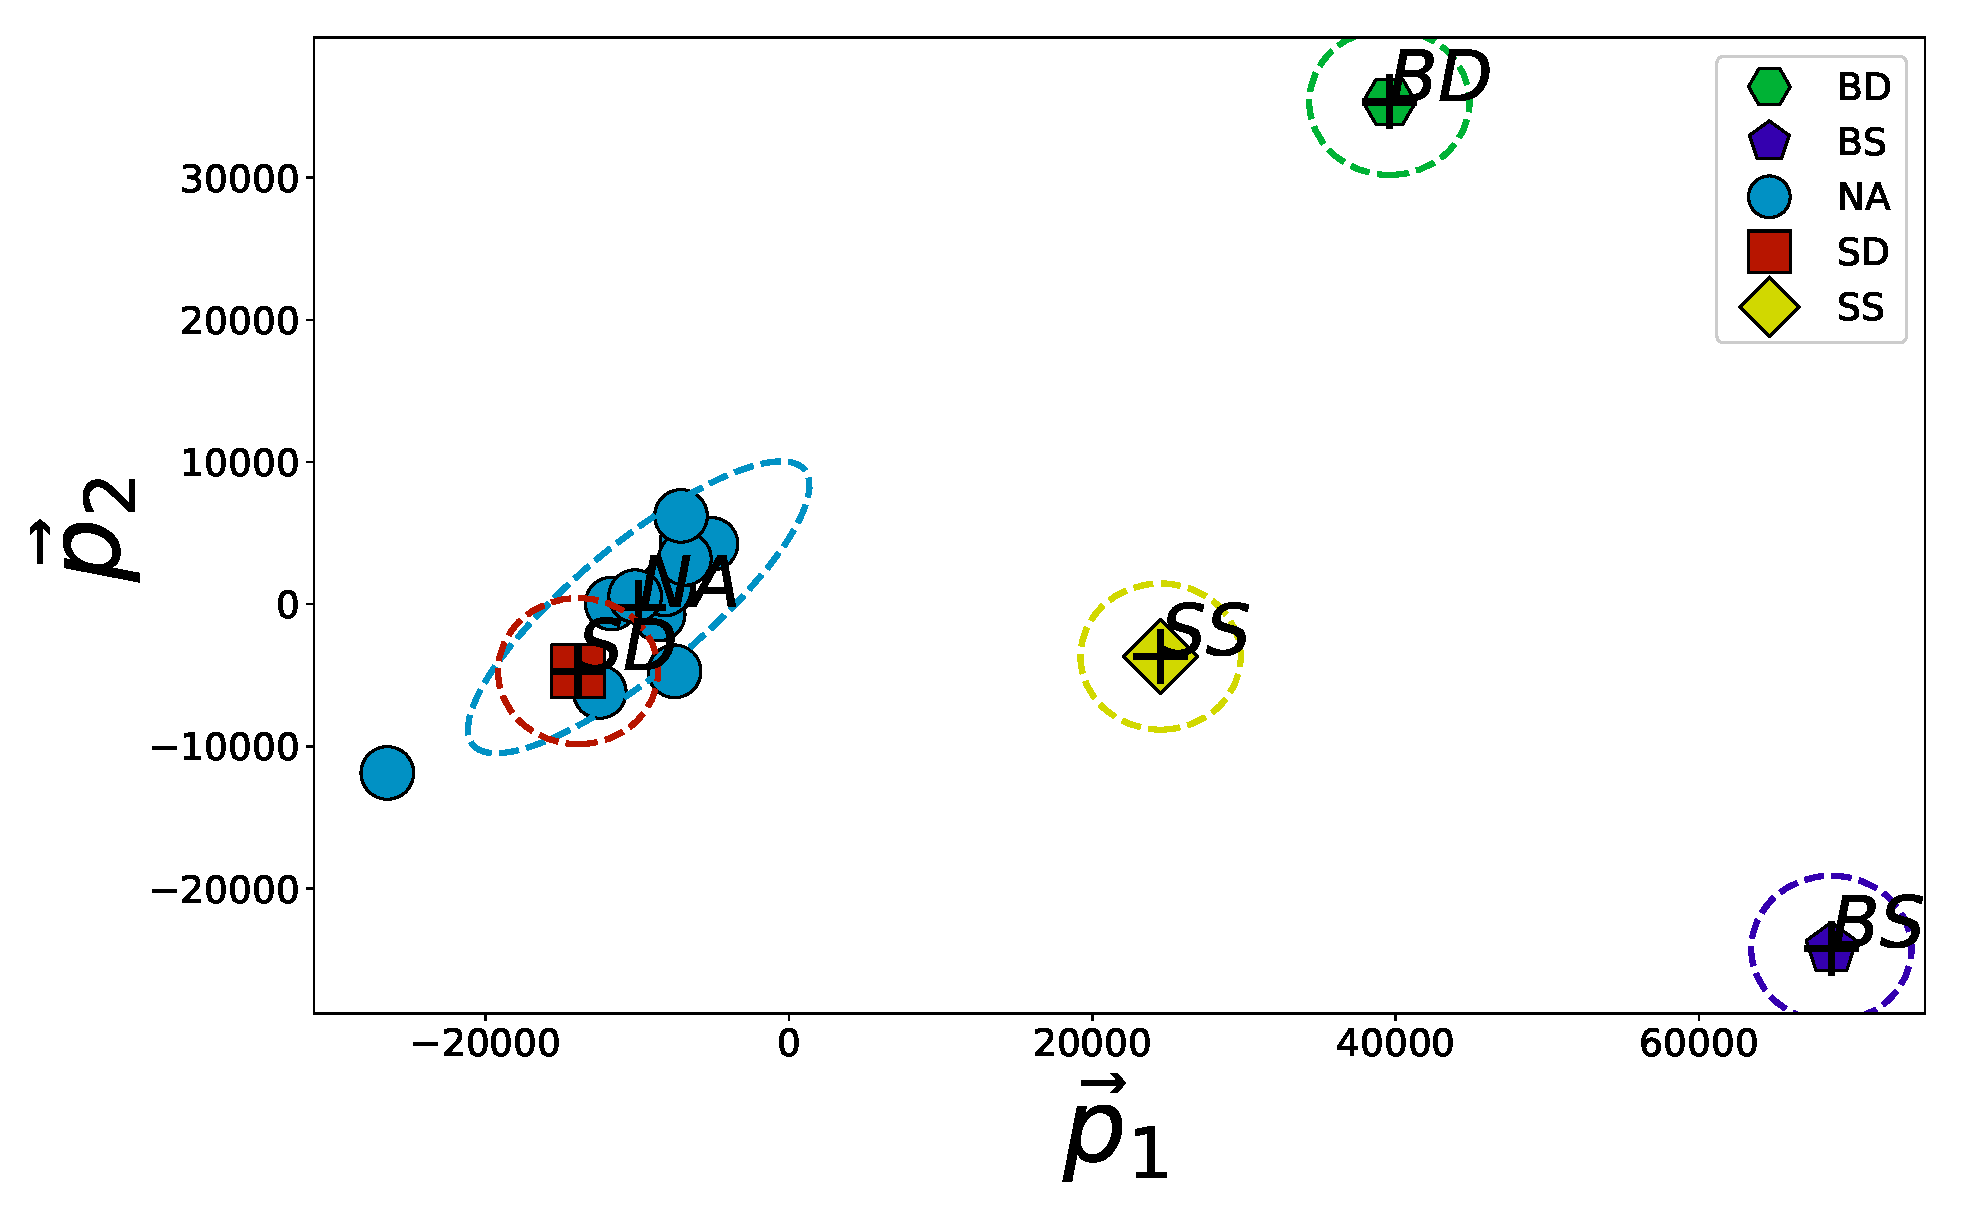
\includegraphics[width=\textwidth]{./figs/phantom1properties_clsplt_Rotate-d160-r160.eps}
			\caption{$\Theta = \small{\begin{Bmatrix}16\\ 16\end{Bmatrix}}$}
			\label{ResRot:160-160}
		\end{subfigure}
	\end{subfigure}
	\caption{The 2-dimensional projection of the tactile information generated from probing $Ph\text{-}2$ 
		at varying depths and radii. The ellipses correspond to the distributions of the clusters based on 
		their true inclusion types, at a distance of 2 standard deviations from their respective cluster center.}
	\label{ResRot}
\end{figure*}

To assess the performance of category formation in each experiment, we first need to match the clusters 
found by the KMC algorithm to any set of target classes for the phantom under analysis. We devise a cluster 
matching process based on maximal accuracy. 

Given the previously computed guess vector $\vec{v}$ and classes $\vec{C}$, 
we first define a function $\Gamma$ such that
\begin{equation}
\Gamma(\vec{v}, \vec{C})=[x |\ x=\vec{C}_{\vec{v}_i} \text{ for } i\in[1,... ,N]] 
\end{equation} 
where $\vec{v}_i$ is the $i^{th}$ element in $\vec{v}$, $\vec{v}_i\in \vec{C}$, and $\vec{C}_{\vec{v}_i}$ is the $\vec{v}_i^{th}$ element in $C$. The function remaps the elements in $\vec{v}$ based on $\vec{C}$.

\begin{figure}[]
	\centering
	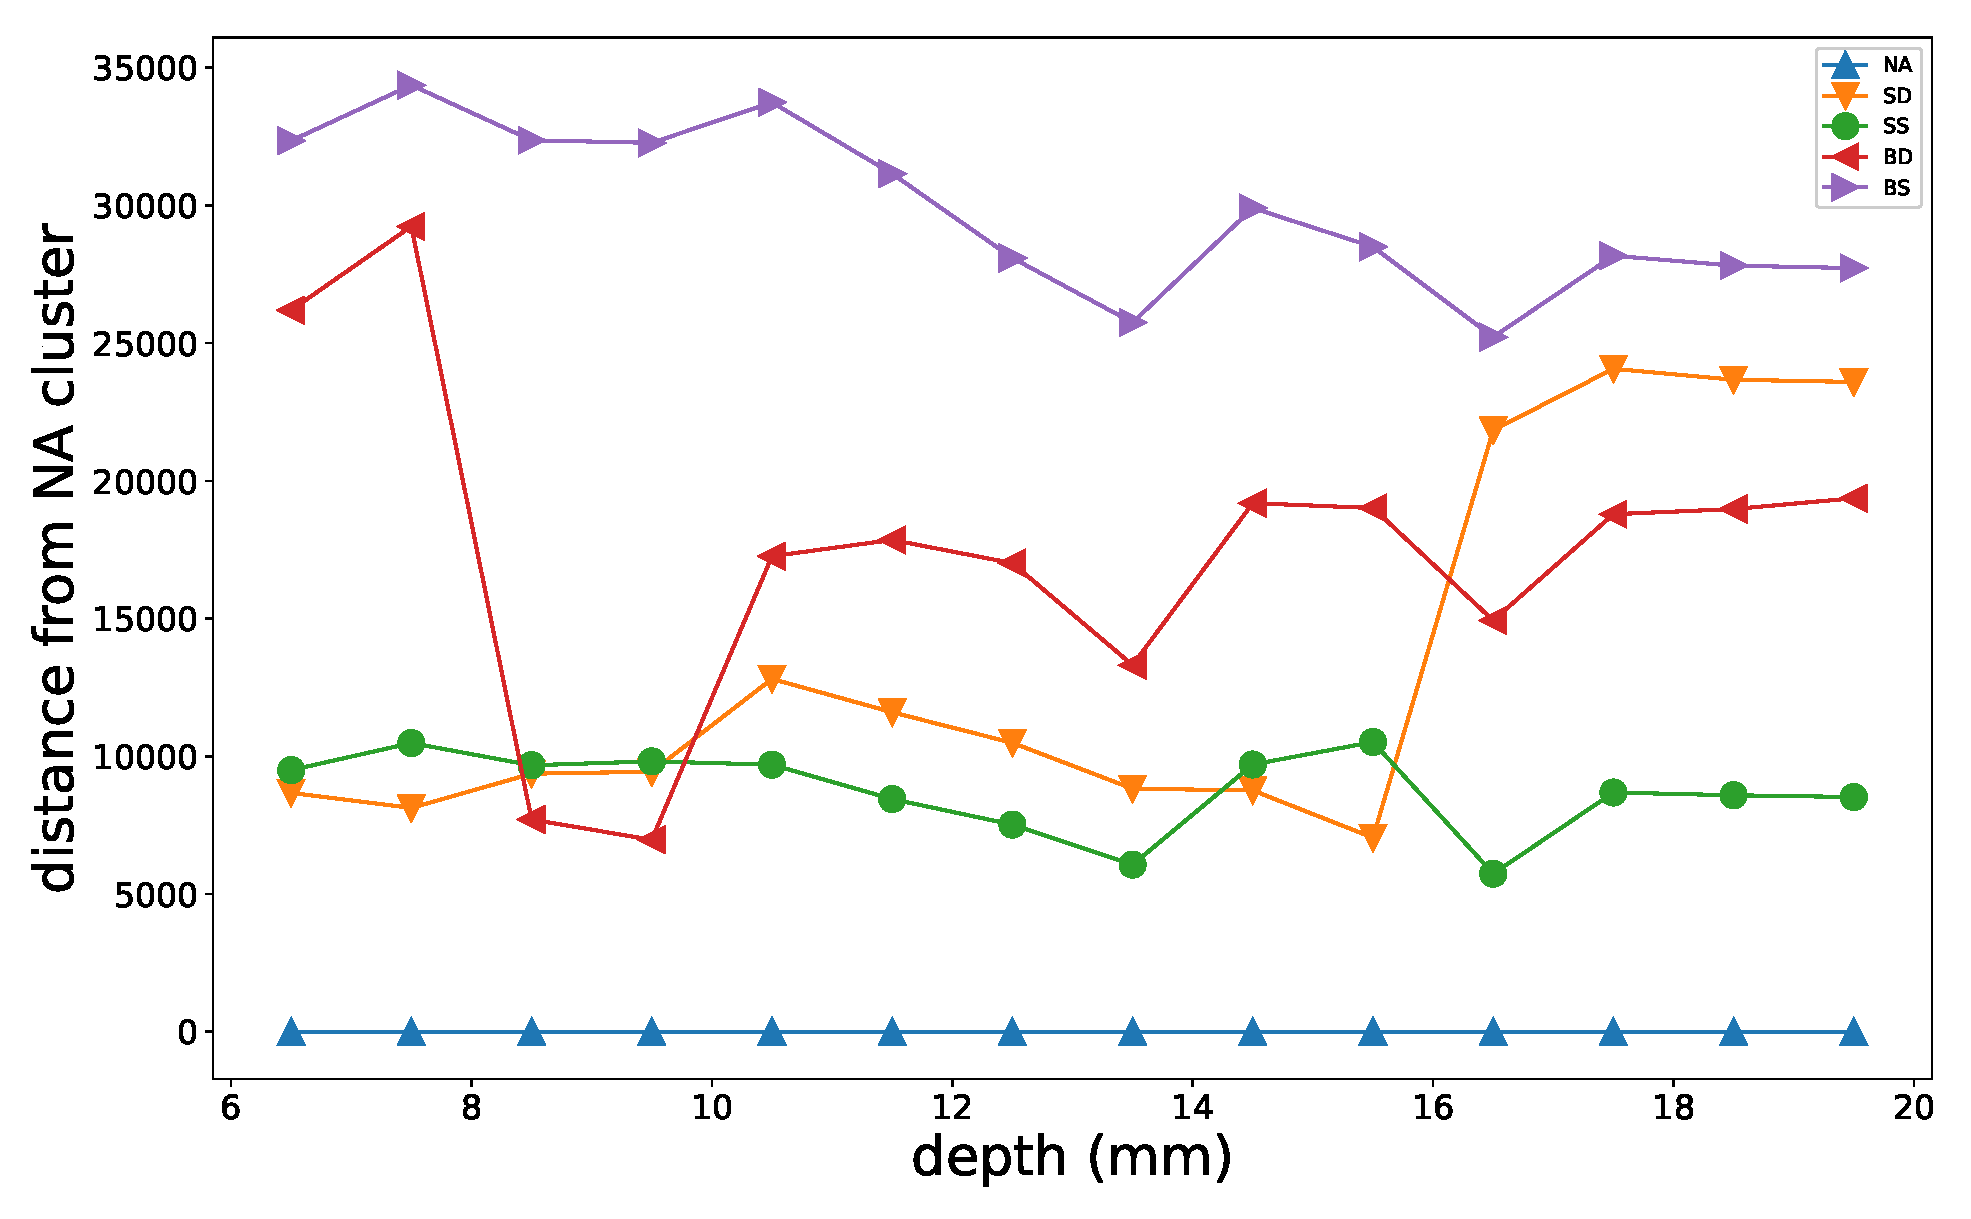
\includegraphics[width=\columnwidth]{./figs/phantom2propertiesVertical_na-dist.eps}
	\caption{The distance between the cluster-matched \textit{NA} cluster and all matched clusters in the data. 
		The data is captured when probing $Ph\text{-}2$ and , setting $r=0$ and varying the $d$ in $\Theta$.}
	\label{na_dist}
\end{figure}

Given a target vector $\vec{t}$ we define a function $\Psi$ to re-associate the classes in $C$ such 
that the distance between the target and the guess vector is minimal, thus:
\begin{flalign*}
\Psi(\vec{v}, \vec{C}) = \operatorname*{argmin}_{\vec{C}^{\ '}} {||\Gamma(t, \vec{C}^{\ '})-\vec{v}||}
\end{flalign*}
where $C^{\ '}\in S(\vec{C})$, $S(C)$ is the set of all permutations of $C$, and $||\cdot||$ is the Euclidean norm of a vector. Finally we define the cluster-matching as:
\begin{equation}
\mathbf{CM}(\vec{v}, \vec{t}, \vec{C}) = \Gamma(\vec{v},\ \Psi(\vec{v}, \vec{C}))
\end{equation}
We use the cluster-matching process to re-associate the cluster memberships
\begin{equation}
\vec{v}^{\ \prime} = \mathbf{CM}(\vec{v}, \vec{t}, \vec{C}).
\end{equation}
Here $\vec{v}\ '$ is a new vector maximizing accuracy for a particular task given (specified by the
target vector $\vec{t}$). A vector $\vec{v}=[2\ 2\ 1\ 0\ 0]$ for a task $\vec{t}=[1\ 1\ 0\ 2\ 2]$, 
for example, would be re-associated as $\vec{v}^{\ \prime}=[1\ 1\ 0\ 2\ 2]$. We utilize the cluster
memberships in $\vec{v}\ '$ to compute each cluster center and retrieve the mutual distances between
clusters.

In this analysis we consider two scenarios where we may want to associate the clusters by depth or size of inclusion, 
and use the \textit{NA} type as ground zero, we thus consider the distance from the cluster-matched 
\textit{NA} inclusion type and the remaining types (Fig. \ref{na_dist}). As clear from Fig. \ref{na_dist}, 
by duly interacting with the soft phantom, the distance between each cluster type and the \textit{NA} 
cluster changes drastically. In this context, then, it is possible to induce a ranked 
understanding of robot's perceived similarities between different inclusion types by simply acting on 
the $\Theta$ parameters.  


\begin{figure}[]
	\centering
	\begin{subfigure}[b]{\columnwidth}
		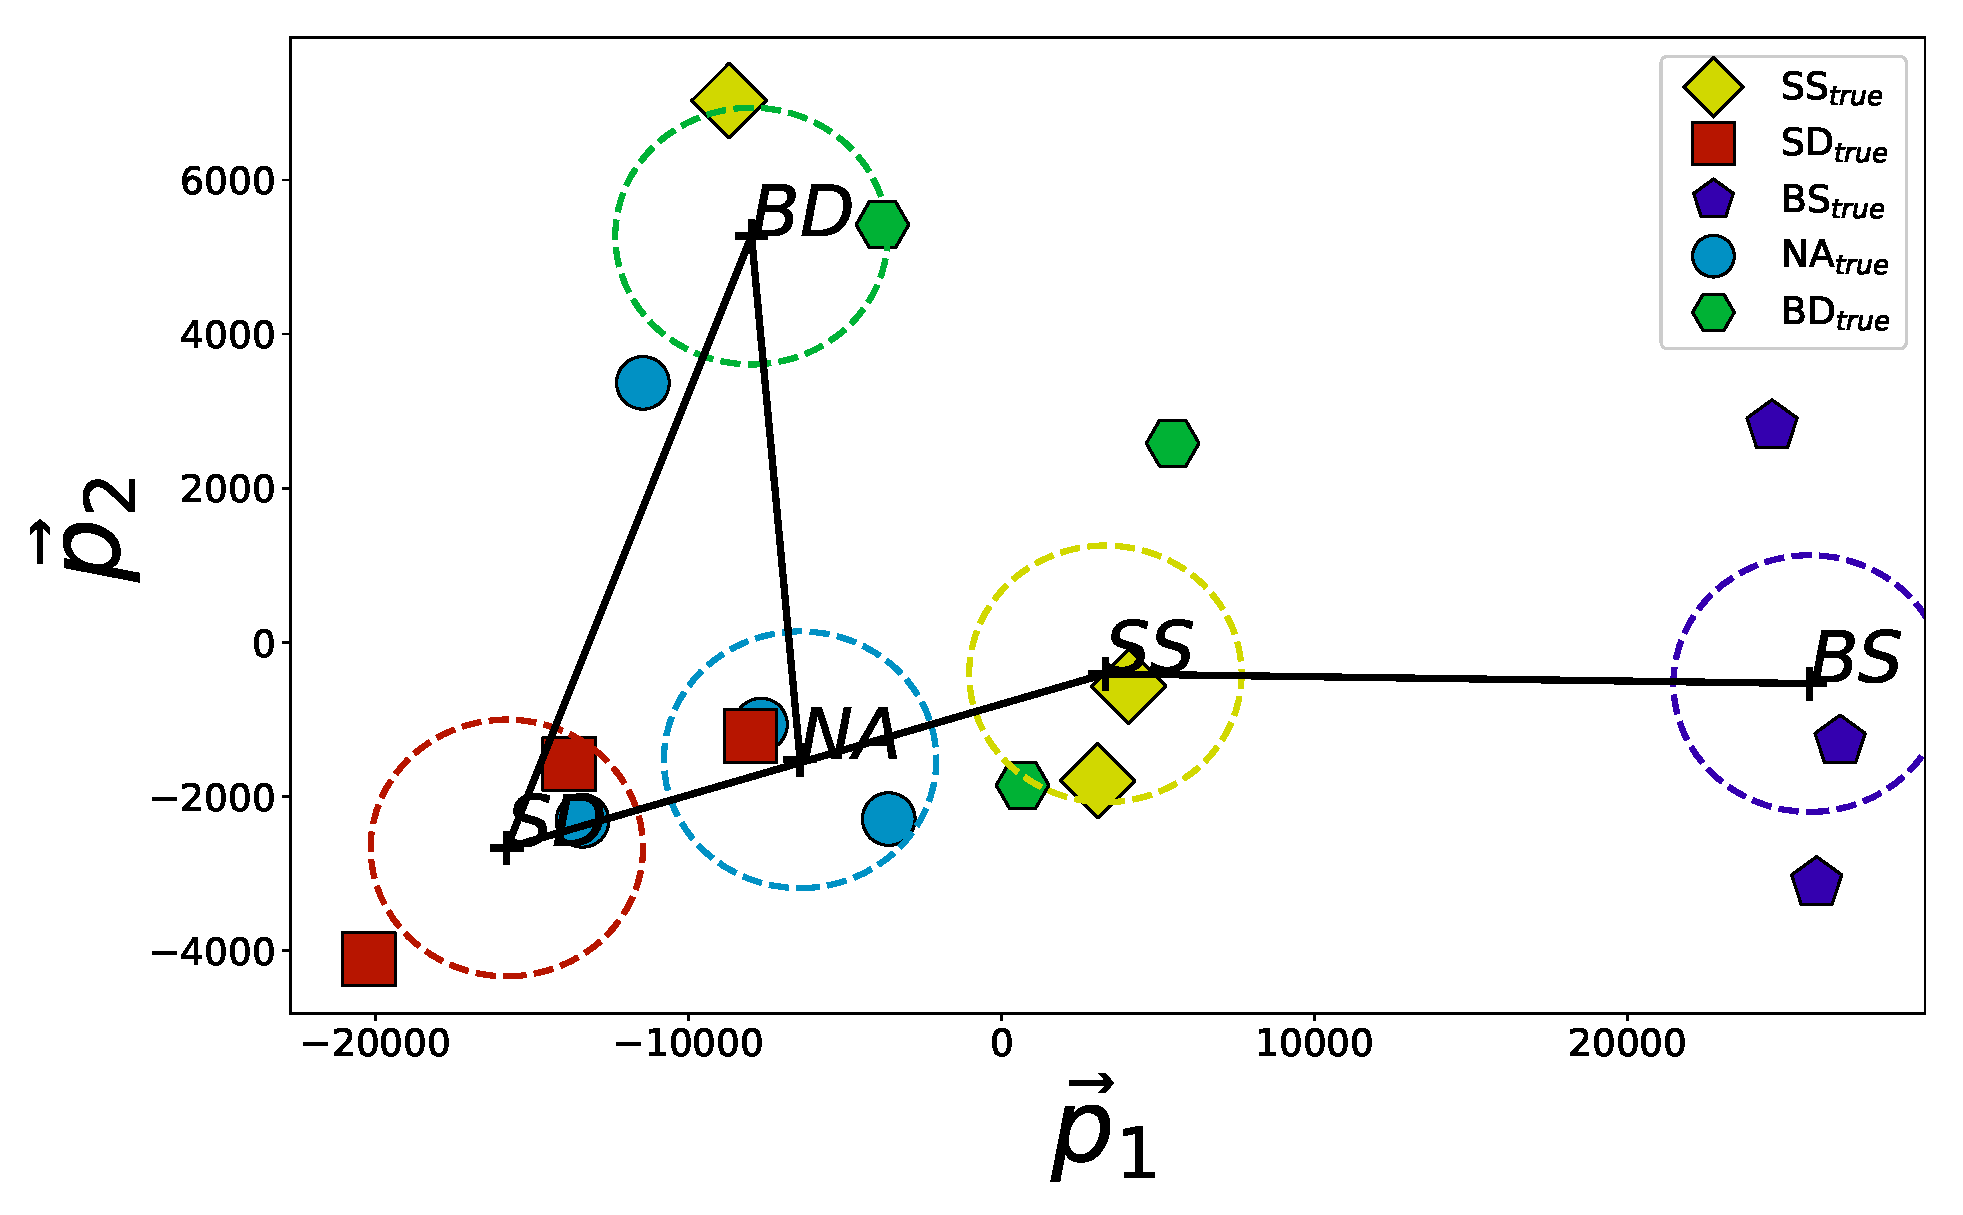
\includegraphics[width=\textwidth]{./figs/phantom2properties_distfig_Vertical-d9_5.eps}
		\caption{$Ph\text{-}2$, $\Theta = \small{\begin{Bmatrix}9.5\\ 0\end{Bmatrix}}$}
		\label{cluster_distance:ph1-1}
	\end{subfigure}
	\begin{subfigure}[b]{\columnwidth}
		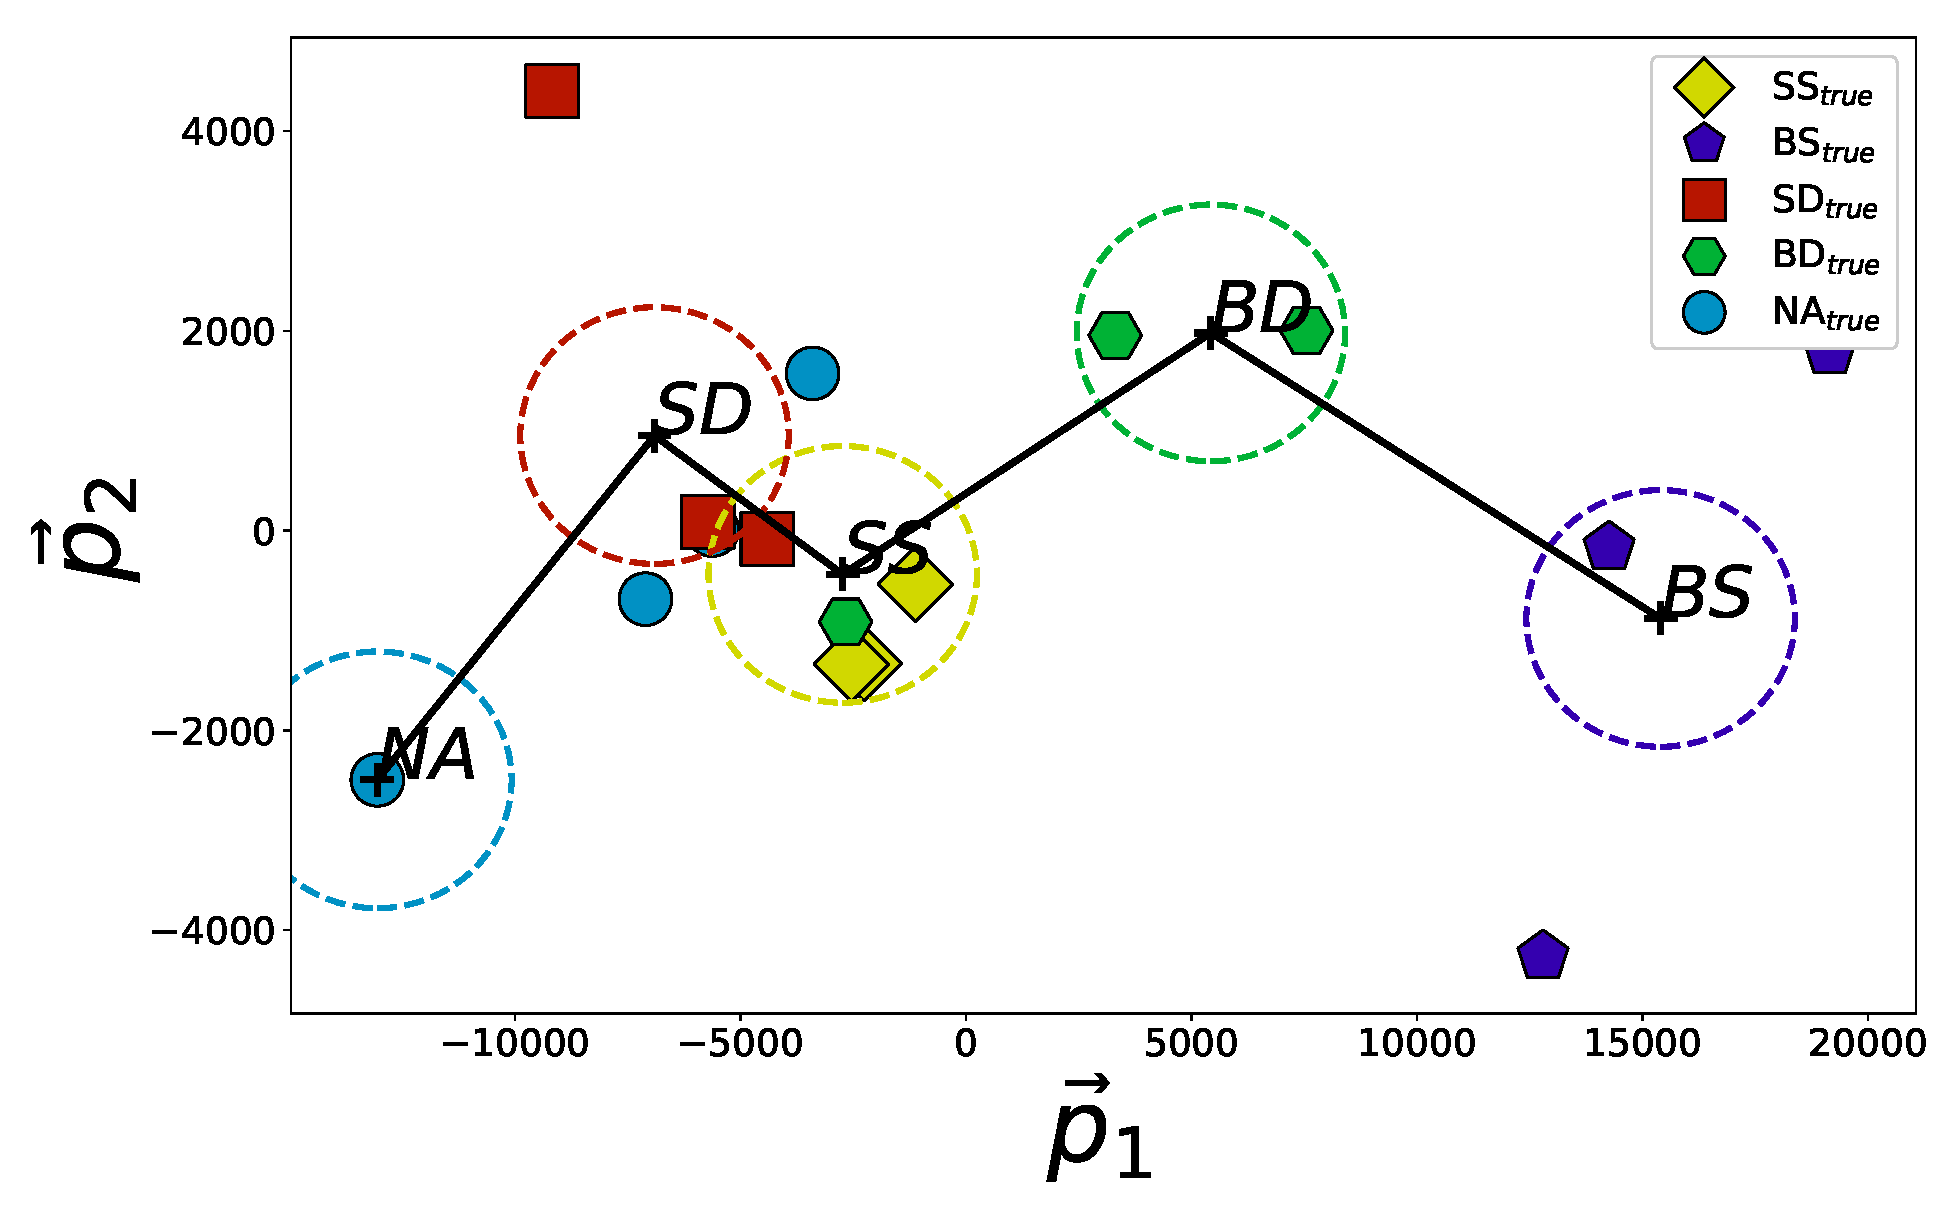
\includegraphics[width=\textwidth]{./figs/phantom2properties_distfig_Vertical-d15_5.eps}
		\caption{$Ph\text{-}2$, $\Theta = \small{\begin{Bmatrix}9.5\\ 0\end{Bmatrix}}$}
		\label{cluster_distance:ph1-2}
	\end{subfigure}
	\caption{The emerging cluster similarities when changing the motion parameters and 
		solving for either rank-1 i.e. $[$\textit{NA}, \textit{SD/BD}, 
		\textit{SS/BS}$]$ (a) or rank-2 i.e. $[$\textit{NA}, \textit{SD/SS}, \textit{BD/BS}$]$ (b). 
		Each dotted circle is placed on the cluster-matched, KMC found, cluster corresponding to the color 
		coding in the legend.}
	\label{cluster_distance}
\end{figure}

We demonstrate the ability to achieve similarity relationships of the kind previously described by 
finding the parameters for which the agent can rank the system based on rank-1 or rank-2. We perform 
the experiments in $Ph\text{-}2$, and we use the experimental data gathered through the probing of the soft 
phantom to find the parameters by which we can solve the ranking. We find the robot capable of 
abstracting similarities relationships according to rank-1 for $\Theta = \tiny{\begin{Bmatrix}9.5\\ 0\end{Bmatrix}}$ (Fig. \ref{cluster_distance:ph1-1}), and according to rank-2 for $\Theta = \tiny{\begin{Bmatrix}15.5\\ 0\end{Bmatrix}}$ (Fig. \ref{cluster_distance:ph1-2}).


\section{Palpation Test Case} \label{sec_test_case}

\color{red}{We perform experiments to test the ability of the framework developed to assess and identify the motion control which can best allow an agent to differentiate among different types of inclusions. For this purpose, the robot is set to perform palpation on a phantom containing $4\text{x}$\textit{NA}, $3\text{x}$\textit{SD}, $3\text{x}$\textit{SS}, $3\text{x}$\textit{BS}, $3\text{x}$\textit{BD}. The sensorized robotic arm is made to palpate the phantom vertically on each location, as described in Section \ref{sec_motor_interactions}.  
At this point, dimensionality reduction is used to pass from a high dimensional sensor description of each palpated phantom location, to a two dimensional descriptor based on PCA analysis (see Section \ref{sec_dim_reduction}).

After dimensionality reduction it is possible to utilize Equations (7) through (9) to assess the quality of each motion strategy with respect to the collected data. The motion strategy parameters generating the highest structure in the data can thus be saved.

Here we make use of a standard classification procedure to dissociate amongst the different types of inclusions, and we assess the ability of the framework described in this paper to assist in determining which motion would have generated the best data for palpation classification.  We use a off-the-shelf multi-class Support Vector Machine (SVM) \cite{cortes1995support} classifier, as implemented in the \emph{scikit-learn} python tool~\cite{scikit-learn}. 

The dataset is composed of 16 different data-points, each corresponding to a 2-dimensional projection of the tactile sensor generated during the palpation of one of the 16 locations in the phantom. Three different type of classification are executed, following the same qualitative analysis in Section \ref{sec_inf_struct}. First a classification with two classes, where the SVM classifier is trained to discriminate between locations containing hard inclusions, and locations with no inclusions. Second, three classes, where the classifier is trained to discriminate between large inclusions, small inclusions or no inclusions. Third, 5 classes, where all inclusion types are considered. For each of the three classification types, the classifier is trained on the minimal possible number of inclusions per class, i.e. 1 sample, and the data-set is split into training and test set accordingly. The split was purposefully chosen to observe the classifier performance when lacking large amounts of data.

After training, the SVM classifier separates the two dimensional space according to the two, three or five classes, maximizing the distance to the nearest training data points of any class. 
Once the classifier has been fit to the training samples, we test the ability of the SVM to classify a new inclusion correctly by testing it on the unseen phantom test locations. 

Fig. \ref{svm_acc} shows the resulting accuracy of the classifier at different probing depths and when classifying the inclusions following the three different sets of classes described. 
Given the difficulty of the classification task with the limited amount of data, the classifier can only achieve an average classification accuracy of 68.78\% when detecting hard inclusions,  36.26\% when detecting inclusions based on size and 47.40\% when discriminating inclusions based on all their properties. Even in this scenario, the motion strategy detected by the proposed framework can achieve accuracies of respectively 78.57\%, 69.23\% and 63.63\% in the same tasks, improving on the average classification accuracy of up to 10-33\%, as shown by the black circles in Fig. \ref{svm_acc}.
%While it is fairly simple to detect an hard inclusion (red plot in Fig. \ref{svm_acc}), it is harder for the agent to classify inclusions based on their size (green plot in Fig. \ref{svm_acc}) or size and depth (blue plot in Fig.  \ref{svm_acc}), i.e. the accuracy decreases with the increase in the number of classes. 
\begin{figure}[]
	\centering
	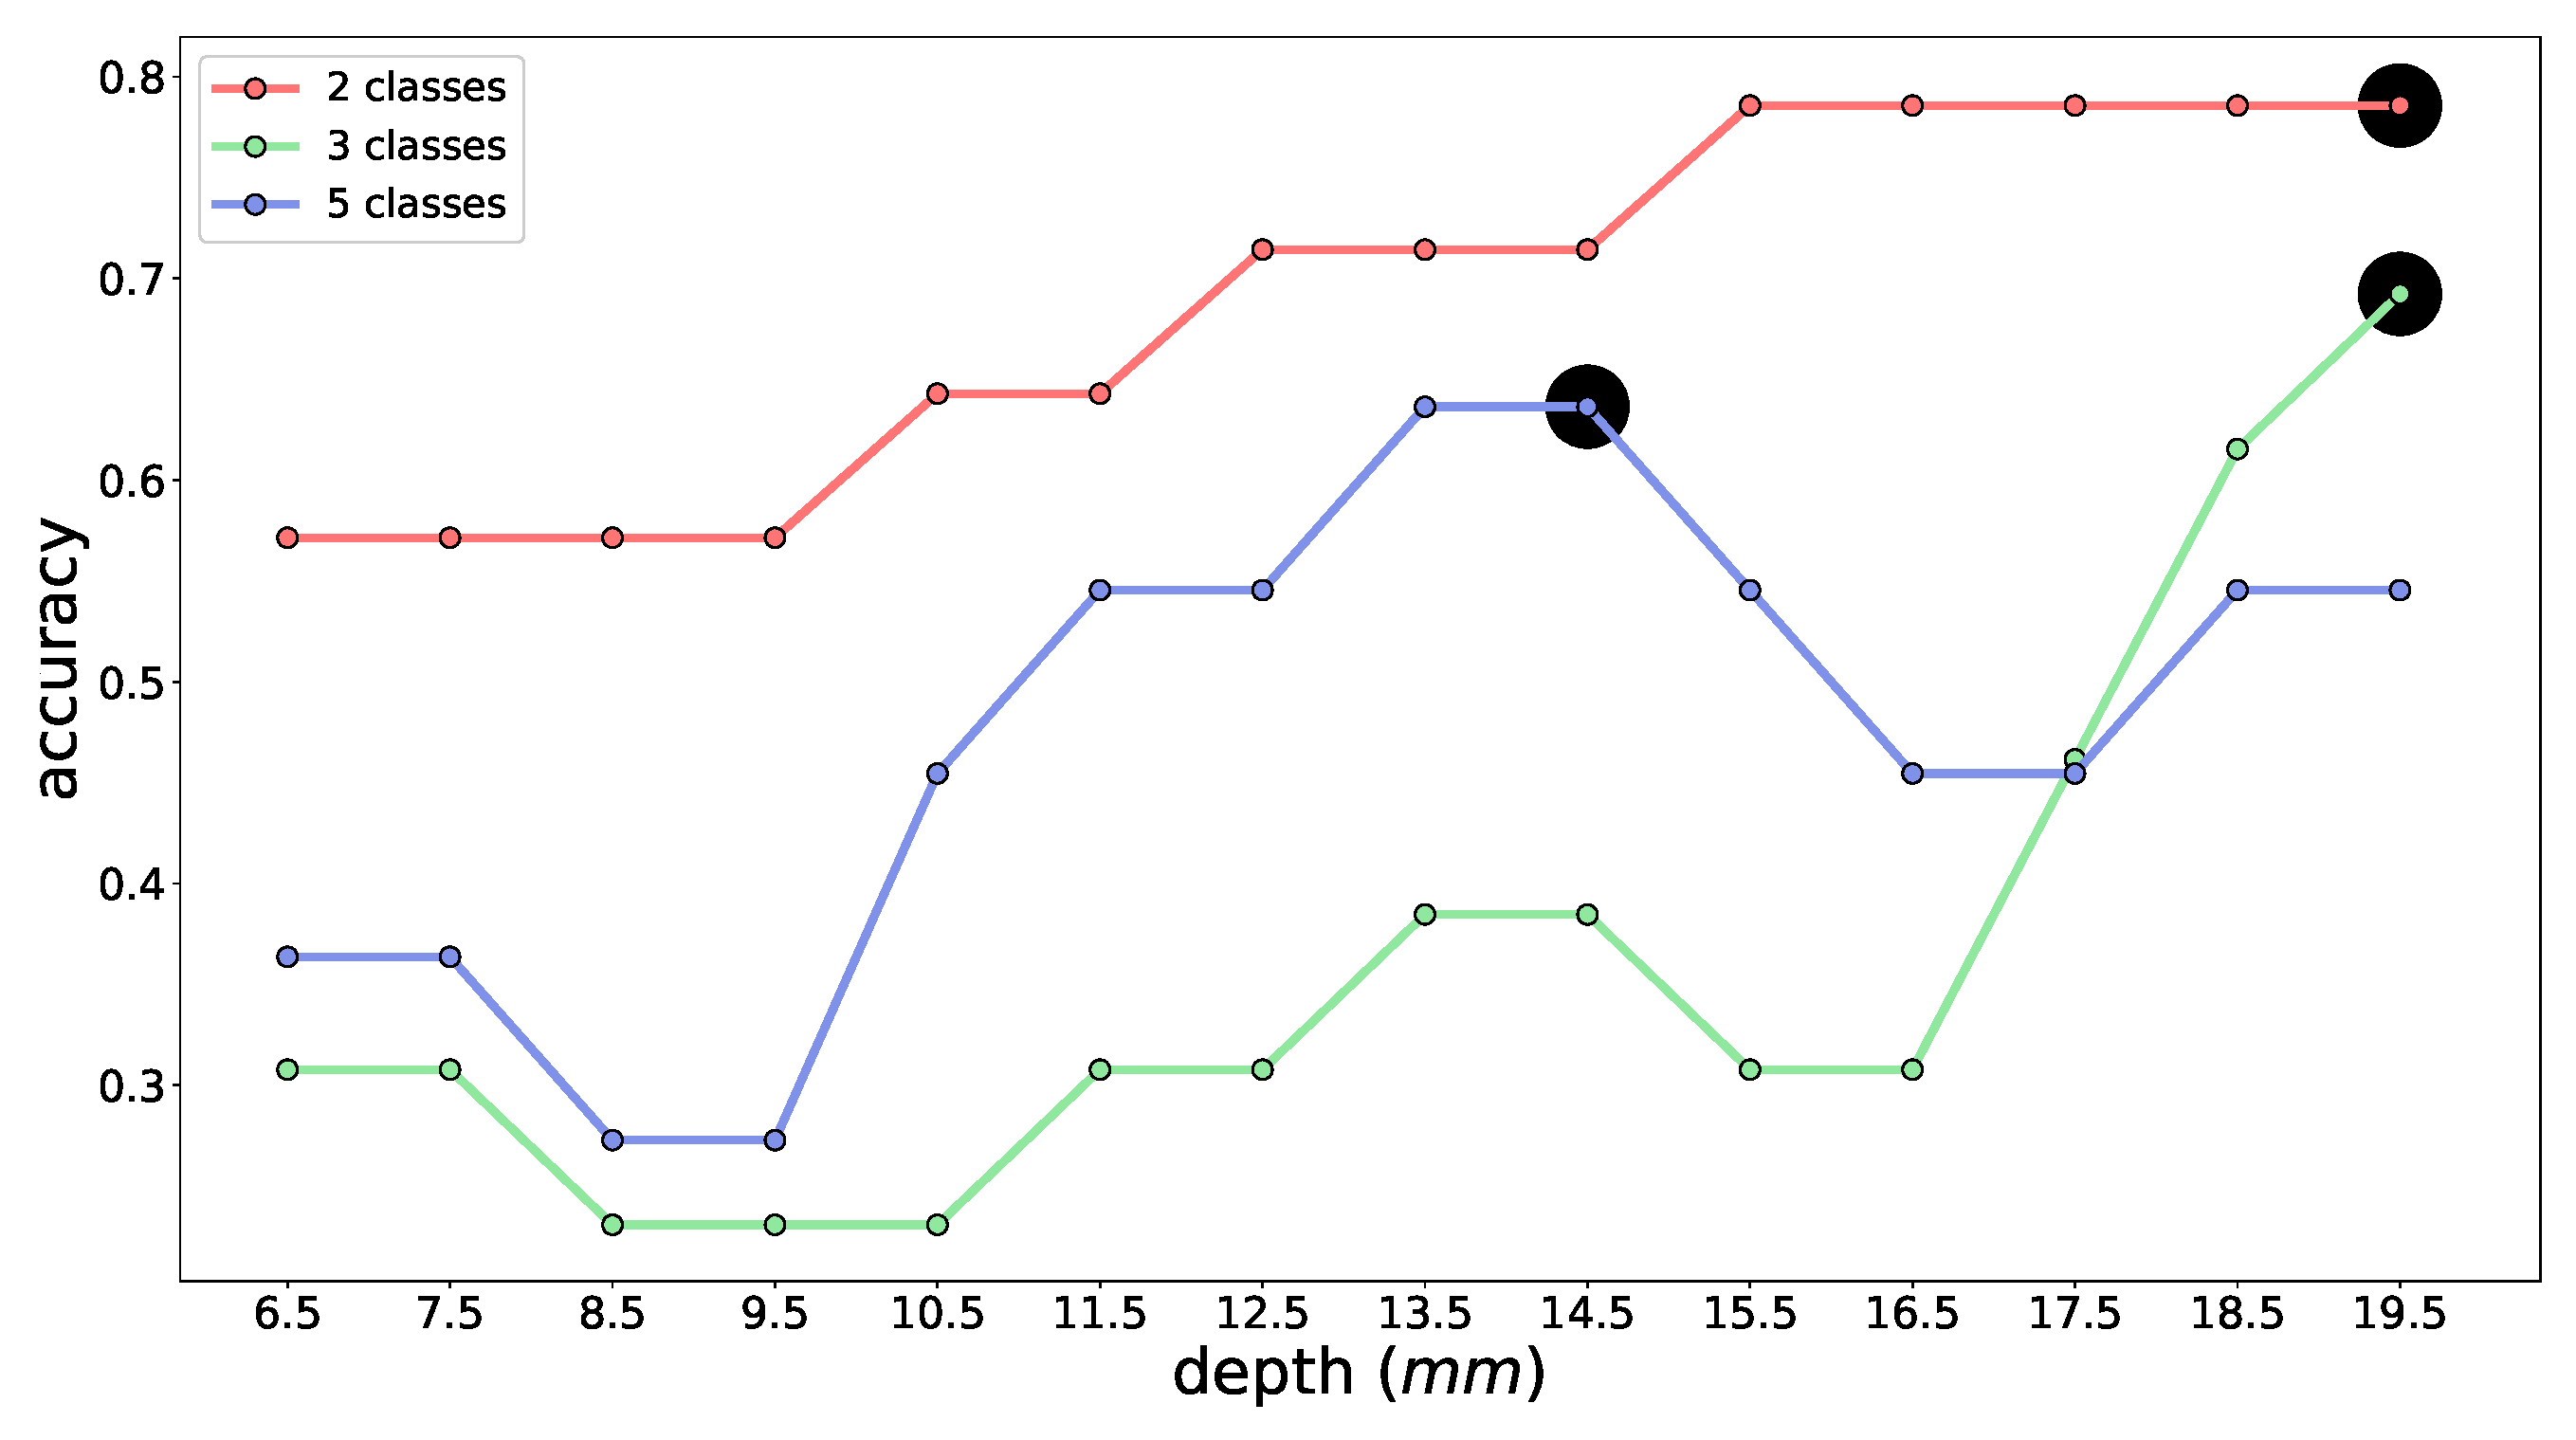
\includegraphics[width=\columnwidth]{./figs/bar_clst_num_change_svm.eps}
	\caption{\color{red}{The classification test accuracy of a multi-class SVM trained on a single sample for each inclusion type, when performing a vertical probing action at different depths, and over varying number of  clusters. The highlighted black circles correspond to the maximal silhouette score computed through the proposed framework (see Fig. \ref{clst_number}).}}
	\label{svm_acc}
\end{figure}
More significantly, when comparing Fig. \ref{clst_number} and Fig. \ref{svm_acc}, it becomes clear how the general performance of the classification can indeed be predicted by the framework proposed, by solely relying on information structure. In fact, additionally to the best performing motion strategy, both the motion parameters resulting in the least accurate classification, as well as the general flow of the accuracy graph in Fig. \ref{svm_acc} can be almost faithfully predicted based on the scores in Fig. \ref{clst_number}.}

\color{black}
\section{Conclusion} 	\label{sec_conclusion}

%Sensory-motor coordination is a fundamental process by which the sensory inputs can be actively changed 
%through interactions with the environment. 
In this paper we investigated the effects of various motion strategies to the response of a capacitive 
tactile sensor, for the task of detecting hard inclusions in a soft body. 
Actively choosing an interaction strategy, to optimize sensory reception for a specific task at hand, has 
the potential to be a powerful tool. Such tool could endow robots with the ability to dynamically filter  
properties of touched objects, actively helping in the completion of a task \cite{olsson2004sensory, bohg2017interactive} 
even before the sensor information arrives to a central processing unit. 

The experiments were performed by embedding a capacitive tactile sensor onto a 3D-printed end-effector, 
and probing two soft phantoms with various hard inclusions through different probing strategies. 
The sequential sensor data obtained through the probing of each area in the phantom was clustered, 
and the change in information due to each strategy observed and analyzed. 

We found the amount of information retained after PCA projection to be highly dependent both on the 
probing strategy and the properties of the sample areas in interaction. More interestingly, 
we found that appropriate probing strategies can help retain information even when lacking a 
large quantity or good quality of it. 
%When considering physical tactile sensor information, it is often necessary to work with high dimensional 
%spatiotemporal information. To pass from a high dimensional sensor-space, to a low dimensional encoding of 
%the sensed objects, much information needs to be discarded. Here, it becomes necessary to have a process 
%capable of driving such process. 
Using the explained variance as a measure of information is useful in ensuring large amount of heterogeneity 
is kept in the data, but it is not capable of ensuring the quality of the information retained. In fact, 
it could be possible that the projection makes the information relative to highly distinct object, 
indistinguishable after projection. However, under the assumption of no prior knowledge of target labels, 
keeping variance in the data is usually a sensible choice.

Furthermore, we analyzed the impact due to motion on cognitive maps and extracted how the motion influenced 
the tactile information. Understanding the effects of motion to the perception of the probed areas 
is necessary to appropriately choose an interaction strategy that generates structure.
To make full use of such effects, however, it would be ideal to instead be able 
to predict such change, before interaction takes place. Here, the change in position 
of each point within a cognitive map could be interpreted as a transformation in the same domain. 
The transformation function could be learned from initial interaction and used in future tasks to 
optimize the sensor response for a specific task. The transformation function, however, would not only be 
dependent on the motion parameters employed, but also on the properties of the sample objects in interaction, 
like demonstrated in the results. 

It is also possible to take categorization one step further and abstract 
similarities between object types from Cognitive Maps. Here we have shown that the physical interaction 
can drive the similarity relationship between objects.
In an unsupervised scenario, the abstractions can be highly informative and can, 
for example, be useful to fix an ordering, via mutual distances, on the sensed object types. 
%The ordering induces the agent's understanding of the objects in interaction to be largely different.  
The object ordering can be purposefully fixed to the agent's advantage. In a real scenario
a practitioner might diagnose the gravity of a detected inclusion based on various features. 
In our fictitious example we show how it is possible for an agent to prioritize over two features by 
simply changing the palpation strategy. 
\color{red}

Finally, a test case of the application of the proposed framework in a classification scenario is presented.
A robot is made to palpate a clustered phantom, and an SVM multi-class classifier is trained on the minimal possible amount of samples per class.
The classifier is shown to perform best when employing the highest scoring motion strategy, as detected by the proposed framework. The chosen strategy is shown to improve the classification accuracy of the classifier of up to 33\%. More interestingly, we observe the silhouette analysis based on our method can predict the general relative performance of the classification a priori. 
\color{black}

%Observing the changing in tactile encoding through the PCA-KMC lens has allowed us 
%to see how a set of motion strategies affected the lower-dimensional encoding of the sensory stimuli for 
%each probed location in a soft phantom. 

%The analysis has brought the understanding of each parameters effectis the change in information 
%obtained when varying the depth of probing for both the motion strategiess employed. This, in fact, 
%not only causes the sensor's response to saturate better over areas with hard inclusions, but unifies 
%the sensor response for areas where no hard inclusion is detected, effectively increasing its certainty over these. 


%\begin{acknowledgements}
%If you'd like to thank anyone, place your comments here
%and remove the percent signs.
%\end{acknowledgements}

% BibTeX users please use one of
\bibliographystyle{spbasic}      % basic style, author-year citations
%\bibliographystyle{spmpsci}      % mathematics and physical sciences
%\bibliographystyle{spphys}       % APS-like style for physics
\bibliography{IEEEexample}

\bigskip


\end{document}
% end of file template.tex


